% !TeX root = ../Book2.tex
% 纲要标题：# 第三编　横截性、相交与 Morse 理论
% 纲要位置：几何学计划纲要.md，第 1536 行。
% 正文状态：本编导读初稿；尚未正式审核。

% 纲要内容开始
% 
% 纲要内容结束

\BookPart{横截性、相交与 Morse 理论}{g2:part:03}
\BookPartGuide
两条曲线相切时，轻微移动就可能让一个交点变成两个，也可能让它消失；横截相交则能在足够小的扰动下保持局部形状。要把相交次数变成拓扑不变量，首先需要控制这种局部变化，再研究一族交点怎样组成带边界的流形。本编由光滑逼近和横截性开始，把代数拓扑中的映射度、对偶和胞腔边界解释为光滑几何中的计数与分解。

\ProseParagraphBreak

\chapref{g2:ch:14}说明如何扰动映射而保留指定区域的数据。Sard 定理使正则值可以被选出，参数横截性则把一族映射的总体性质转为大多数参数下的性质。这样得到的逆像具有预期维数，横截同伦的逆像还会提供配边。\chapref{g2:ch:15}处理相邻的构造问题：怎样把抽象流形嵌入 Euclid 空间，怎样用法丛描述子流形的整个邻域，以及怎样把子流形的运动延拓为环境运动。固有满淹没的局部平凡性也在这里证明；其核心是保证沿基底道路的全部提升能够走完所需时间。

\ProseParagraphBreak

有了横截性和邻域模型，\chapref{g2:ch:16}便能把正则值原像、子流形交点和向量场零点赋予符号。改变正则值或扰动时，点集连成一维配边；边界的符号关系给出计数的不变性。前面由基本类与杯积定义的配对，在这里得到横截代表的解释。不动点也可作为映射图像与对角线的交点处理，从而把局部指数之和与上同调上的交错迹联系起来。

\ProseParagraphBreak

\chapref{g2:ch:17}用一个光滑实函数逐层观察流形。次水平集在没有临界值的区间内沿梯度流变形；越过一个非退化临界点时，局部二次型的负方向决定附着把手的指标。把手给出胞腔同伦模型，临界点数因而受到同调的约束。\chapref{g2:ch:18}继续记录临界点之间的负梯度轨线，以轨线计数建立 Morse--Smale 同调。这里需要分析轨线断裂、紧性和粘合，才能把一维轨线空间的端点与微分平方为零对应起来。正文先用模二系数完成构造与比较，再讨论整数取向。

\ProseParagraphBreak

本编可从第一卷的光滑流形理论直接开始：\chapref{g2:ch:14}、\chapref{g2:ch:15}需要第一卷第11章的微分与子流形坐标、第12章的单位分解，以及第13章的常微分方程存在性和光滑依赖；Sard 证明还用到 Taylor 估计、零测集与 Fubini 定理。进入\chapref{g2:ch:16}时，需要回顾本卷\chapref{g2:ch:04}、\chapref{g2:ch:06}的乘积、帽积与对偶，映射度的同调与积分比较还分别使用\chapref{g2:ch:03}的映射度和\chapref{g2:ch:07}的 de Rham 同构。Morse 不等式和 Morse 同调的比较使用\chapref{g2:ch:03}的胞腔链。前一编的全部谱序列计算并非这些构造的共同前提。阅读时可以沿用同一张曲面：先选择横截曲线计算相交，再选高度函数观察把手附着，最后比较临界点之间的轨线与胞腔边界。这样能够具体辨认局部微分条件怎样约束整体拓扑。

% !TeX root = ../../Book2.tex
% 纲要标题：## 第14章　光滑逼近、Sard 与横截性
% 纲要位置：几何学计划纲要.md，第 1538 行。
% 正文状态：初稿；尚未正式审核。

% 纲要内容开始
% 
% > 本章目标与证明范围：先建立光滑逼近与函数空间的必要拓扑，再完成 Sard 和参数横截性。一般位置的结论具有明确正则性、紧性、相对保持和边界条件。
% 
% 纲要内容结束

\chapter{光滑逼近、Sard 与横截性}
\label{g2:ch:14}
\BookChapterNumber{g2:ch:14}

\begin{chapterabstract}
	方程的解集何时成为流形，以及不规则的相交能否通过微小改变变得规则，是本章的两个基本问题。先以卷积、单位分解和坐标内替换证明相对光滑逼近，说明紧源与非紧源上导数控制的含义；再以秩分层、覆盖估计和维数归纳证明光滑 Sard 定理。横截性将正则值推广到子流形约束，给出逆像的维数、切空间及法丛。参数定理把总体横截化为几乎处处切片横截，局部扰动进一步给出保持闭集附近数据的横截逼近。最后处理边界条件，并由横截同伦构造逆像间的配边。
\end{chapterabstract}

\begin{learninggoals}
	\begin{itemize}
		\item 用局部卷积与截断构造光滑逼近，说明相对条件如何在拼接中保持。
		\item 区分 \(C^0\)、\(C^1\) 及更高阶控制，辨认非紧源上的弱拓扑、强拓扑与紧支改动。
		\item 重建光滑 Sard 定理的证明，并说明临界点集与临界值集的差别及有限可微性的作用。
		\item 将横截条件化为法方向上的满射，计算横截逆像的切空间、维数及法丛。
		\item 从约束流形到参数空间的投影证明参数横截定理，区分稠密、剩余与几乎处处。
		\item 构造相对横截扰动，核对边界限制映射，并用紧性将同伦逆像变成配边。
	\end{itemize}
\end{learninggoals}

考虑平面中的方程 \(y=x^2\) 与直线 \(y=a\)。当 \(a>0\) 时，它们交于两点，每个交点的切线方向都不同；当 \(a<0\) 时没有交点；在 \(a=0\) 时，两点合并成一个相切点。交点数在这个特殊时刻改变，但把参数也加进去，全部解组成的集合 \(\{(a,x):a=x^2\}\) 始终是一条光滑曲线。微分拓扑经常利用这一转换：单个对象可能出现退化，放进一个有足够参数的光滑族后，可以研究哪些切片仍然规则，以及规则切片之间如何联系。

\ProseParagraphBreak

第一卷第11章的正则水平集定理已经说明：当方程组的微分满射时，解集具有预期维数。现在还要回答两个问题。第一，正则值是否足够多，以至于总能作很小的调整选到它？Sard 定理\footnote{Arthur Sard（1909—1980），美国数学家，研究临界值、线性逼近与样条。}给出“临界值为零测集”的答案。第二，约束若是一条曲线或一张曲面，而非一个目标点，什么条件代替满射？所需条件是映射微分的像与约束子流形的切空间共同张成整个目标切空间，即横截性。

\ProseParagraphBreak

本章使用第一卷第11章的微分、逆函数定理和子流形坐标，第12章的局部有限单位分解与光滑截断；具体调用时会恢复条件。分析方面使用紧集上的一致连续性、Taylor 估计以及 Lebesgue 零测集和 Fubini 定理，所需含义在证明处交代。本章的 Sard 与横截性主干针对光滑映射，光滑逼近同时控制任意指定的有限阶导数；最优有限阶 Sard 条件在第14.2节准确陈述并注明原论文的证明位置。有关光滑逼近和参数横截性的参考见\cite[第6章]{Lee2012Smooth}。

% !TeX root = ../../Book2.tex
% 纲要标题：### 14.1 光滑逼近及函数空间
% 纲要位置：几何学计划纲要.md，第 1542 行。
% 正文状态：未撰写；本文件目前是框架。

% 纲要内容开始
% 
% * 局部卷积和单位分解
% * 保持闭子集附近数据的相对逼近
% * 紧源上的 Cʳ 拓扑
% * 非紧源上支集与拓扑的选择
% 
% 纲要内容结束

\section{光滑逼近及函数空间}
\label{g2:sec:1401}

待撰写

\subsection{局部卷积和单位分解}
\label{g2:subsec:1401:01}
待撰写

\subsection{保持闭子集附近数据的相对逼近}
\label{g2:subsec:1401:02}
待撰写

\subsection{\texorpdfstring{紧源上的 \(C^r\) 拓扑}{紧源上的 Cʳ 拓扑}}
\label{g2:subsec:1401:03}
待撰写

\subsection{非紧源上支集与拓扑的选择}
\label{g2:subsec:1401:04}
待撰写
% 纲要条目排为编号小节标题，并进入目录与书签；说明段仍保留于纲要注释中。

% !TeX root = ../../Book2.tex
% 纲要标题：### 14.2 Sard 定理的证明
% 纲要位置：几何学计划纲要.md，第 1549 行。
% 正文状态：初稿；尚未正式审核。

% 纲要内容开始
% 
% * 临界集合的秩分层
% * 秩为零部分的覆盖估计
% * 维数归纳与 Fubini 步骤
% * 正则性阶数及反例范围
% 
% 纲要内容结束

\section{Sard 定理的证明}
\label{g2:sec:1402}

方程 \(f(x)=y\) 的解集能否成为光滑子流形，取决于解上的微分是否满射。单独检查一个指定的 \(y\) 可能很难；Sard 定理给出整体信息：对光滑映射，坏的目标值只占一个零测集。证明必须控制临界点的\emph{像}，因为源中的临界点本身可能很多，甚至充满整个源流形。

\subsection{临界集合的秩分层}
\label{g2:subsec:1402:01}

先明确这里的“坏”。设 \(f:M^m\to N^n\) 是 \(C^1\) 映射，\(N\) 无边界。若 \(\mathrm{d}f_x:\mathrm{T}_xM\to\mathrm{T}_{f(x)}N\) 不满射，称 \(x\) 为\term{临界点}[critical point]；否则称为\term{正则点}[regular point]。临界点的像称为\term{临界值}[critical value]。若 \(f^{-1}(y)\) 中每一点都正则，称 \(y\) 为\term{正则值}[regular value]。特别地，不在像中的点也是正则值；一个值只要有一个临界原像，就已经是临界值。

\ProseParagraphBreak

在 \(n\) 维流形 \(N\) 中，集合 \(E\) 称为\term{零测集}[set of measure zero]，若它在每张坐标图中的像都有 \(n\) 维 Lebesgue 测度零。Euclid 空间中的含义是：给定任意 \(\varepsilon>0\)，能用可数个长方体覆盖它，并使体积总和小于 \(\varepsilon\)。这个条件与坐标无关。在较小的紧坐标块上，光滑坐标变换的导数有界，因而是 Lipschitz 映射；一个半径为 \(r\) 的小球的像落在半径至多为 \(Lr\) 的球中，覆盖总体积至多乘上固定常数。再用可数个这样的坐标块覆盖，便知零测性保持。这里用的是同维坐标变化，无须先在 \(N\) 上选择体积形式。

\begin{example}\label{g2:exm:sard-critical-values}
	映射 \(f:\mathbb R^2\to\mathbb R^2\)，\(f(x,y)=(x,y^2)\)，有
	\[
		\mathrm{D}f_{(x,y)}=\begin{pmatrix}1&0\\0&2y\end{pmatrix}.
	\]
	临界点集是 \(y=0\)，临界值集是目标中的横轴。第二坐标为正的值有两个正则原像，第二坐标为负的值没有原像；这两类值都正则。对于常值映射 \(M\to\mathbb R\)，整个 \(M\) 都由临界点组成，临界值却只有一个。
\end{example}

在坐标域 \(U\subset\mathbb R^m\) 内写 \(C=\{x:\operatorname{rank}\mathrm{D}f_x<n\}\)，并按秩分为
\[
	C^{(q)}=\{x:\operatorname{rank}\mathrm{D}f_x=q\},\qquad 0\le q<n.
\]
这些集合未必都是子流形。分层在这里首先是一种分类：当 \(q\ge1\) 时，某个非零的偏导数让我们把一个输出坐标直接改作输入坐标，进而把问题降低一维。

\begin{lemma}\label{g2:lem:sard-rank-reduction}
	设 \(f:U\to\mathbb R^n\) 光滑，\(U\subset\mathbb R^m\) 开，且 \(\operatorname{rank}\mathrm{D}f_a\ge1\)。重排坐标后，在 \(a\) 的某个邻域上存在光滑源坐标 \((t,z)\in J\times V\subset\mathbb R\times\mathbb R^{m-1}\)，使
	\[
		f(t,z)=(t,G(t,z)),\qquad
		\operatorname{rank}\mathrm{D}f_{(t,z)}=1+\operatorname{rank}\mathrm{D}_zG(t,z).
	\]
\end{lemma}
\begin{proof}
	选择非零偏导数并重排坐标，使 \(\partial f^1/\partial x^1(a)\ne0\)。令
	\[
		\Phi(x)=\bigl(f^1(x),x^2,\ldots,x^m\bigr).
	\]
	其导数行列式正是这个非零偏导数。第一卷第11章第3节的逆函数定理保证 \(\Phi\) 在充分小的邻域上可光滑反解；缩小像邻域，可取乘积盒 \(J\times V\)。在新坐标中，第一分量为 \(t\)，其余分量记作 \(G\)，于是
	\[
		\mathrm{D}f=\begin{pmatrix}1&0\\\partial_tG&\mathrm{D}_zG\end{pmatrix}.
	\]
	利用第一行消去第一列下方的元素，矩阵的秩便等于 \(1+\operatorname{rank}\mathrm{D}_zG\)。
\end{proof}

这里没有要求邻域内的秩恒定；非零偏导数只负责选出一个可用的坐标。真正需要继续处理的，正是其余方向上仍会变化的秩。

\subsection{秩为零部分的覆盖估计}
\label{g2:subsec:1402:02}

若 \(\mathrm{D}f_a=0\)，上面的坐标办法暂时失效。此时 Taylor 展开提供另一种控制：若若干阶导数都为零，一个边长为 \(\delta\) 的源立方体的像就比 \(\delta\) 小得多。源中小立方体的数量约为 \(\delta^{-m}\)，而每个像的 \(n\) 维体积约为 \(\delta^{n(k+1)}\)；当后一个指数更大时，总体积趋于零。

\begin{lemma}\label{g2:lem:sard-flat-cover}
	设 \(U\subset\mathbb R^m\) 开，\(m,n\ge1\)，\(f:U\to\mathbb R^n\) 为 \(C^{k+1}\) 映射，\(k\ge1\)。令
	\[
		A_k=\{x\in U:\partial^\alpha f^i(x)=0\text{，对所有 }1\le|\alpha|\le k,\ 1\le i\le n\}.
	\]
	若 \(n(k+1)>m\)，则 \(f(A_k)\) 为零测集。
\end{lemma}
\begin{proof}
	用可数个包含于 \(U\) 的闭立方体覆盖 \(U\)，只需在其中一个闭立方体 \(Q\) 上证明结论。\(Q\) 上各个 \(k+1\) 阶偏导数有共同的上界。将边长为 \(R\) 的 \(Q\) 均分成 \(s^m\) 个边长 \(R/s\) 的小立方体。对每个与 \(A_k\) 相交的小立方体 \(Q_j\)，选取 \(a_j\in A_k\cap Q_j\)。Taylor 公式的低阶项全部为零，故存在与 \(s,j\) 无关的常数 \(B\)，使
	\[
		|f(x)-f(a_j)|\le B|x-a_j|^{k+1}
		\le B\bigl(\sqrt m R/s\bigr)^{k+1}\qquad(x\in Q_j).
	\]
	因此 \(f(A_k\cap Q)\) 被至多 \(s^m\) 个半径为 \(B(\sqrt m R/s)^{k+1}\) 的球覆盖。若 \(\omega_n\) 表示单位 \(n\) 维球的体积，覆盖总体积至多为
	\[
		s^m\omega_n B^n(\sqrt m R/s)^{n(k+1)}
		=C_Qs^{m-n(k+1)}\longrightarrow0.
	\]
	零测性由此成立；可数并仍为零测集，故得到整个 \(A_k\) 的结论。
\end{proof}

这里的多重指标 \(\alpha=(\alpha_1,\ldots,\alpha_m)\) 记录各坐标求导次数，\(|\alpha|=\alpha_1+\cdots+\alpha_m\)。上式只需普通的有限阶 Taylor 余项估计，不要求函数等于自己的 Taylor 级数。对于光滑函数，在一点的全部导数都为零也不能推出其在邻域内恒定；例如 \(e^{-1/x^2}\) 在 \(x=0\) 补值为零后的函数就具有这种现象。覆盖估计恰好能处理这些极其平坦的点。

\subsection{维数归纳与 Fubini 步骤}
\label{g2:subsec:1402:03}

剩下的工作是把前面两种控制接起来。正秩部分沿一个输出坐标切片；零秩但尚未高度平坦的部分，则落在某个偏导数的正则零集上。两种情形都把源的维数减少一。

\ProseParagraphBreak

切片时使用如下 Fubini 结论：若 \(E\subset\mathbb R\times\mathbb R^{n-1}\) 紧，\(n\ge2\)，且每个截面 \(E_t=\{w:(t,w)\in E\}\) 都为 \((n-1)\) 维零测集，则 \(E\) 为 \(n\) 维零测集。因为紧集是 Borel 可测集，对其示性函数使用非负函数的 Fubini--Tonelli 定理，得到
\[
	\operatorname{vol}_n(E)=\int_{\mathbb R}\operatorname{vol}_{n-1}(E_t)\,\mathrm{d}t=0.
\]
这一紧集切片结论也有只用有限覆盖的证明，见\cite[第126页，引理6.2]{Lee2012Smooth}。下面每次都先限制到紧块，使所处理的像确实可测。

\begin{theorem}[Sard 定理]\label{g2:thm:sard}
	设 \(M^m\) 是有限维、Hausdorff、第二可数的光滑流形，允许有边界；\(N^n\) 是无边界光滑流形，具有相同的分离性与可数性条件。若 \(f:M\to N\) 光滑，则它的临界值集在 \(N\) 中为零测集。因此正则值在 \(N\) 中稠密。
\end{theorem}
\begin{proof}
	先证明无边界情形，并对源维数 \(m\) 归纳。当 \(n=0\) 时，所有微分都满射，临界值集为空。当 \(m=0<n\) 时，第二可数的零维流形是可数离散集，像也可数，故为零测集。以下设 \(m,n\ge1\)，并假设所有源维数小于 \(m\) 的光滑映射均已满足结论。

	取可数的源、目标坐标图，并将源图限制在各目标图的原像内。坐标变化保持微分的秩和目标零测性，故只需讨论 \(f:U\subset\mathbb R^m\to\mathbb R^n\)。除临界集 \(C\) 外，记 \(A_j\) 为前一引理中一至 \(j\) 阶偏导数全为零的集合。它们在 \(U\) 内闭，并满足
	\[
		C\supset A_1\supset A_2\supset\cdots.
	\]
	取整数 \(k\ge1\) 使 \(n(k+1)>m\)。我们依次处理
	\[
		C=(C\setminus A_1)\cup\bigcup_{j=1}^{k-1}(A_j\setminus A_{j+1})\cup A_k.
	\]

	对 \(C\setminus A_1\)，若 \(n=1\)，此集合为空：一维目标的微分不满射就只能为零。若 \(n\ge2\)，\cref{g2:lem:sard-rank-reduction}在每个这样的点附近给出 \(f(t,z)=(t,G(t,z))\)。令 \(G_t(z)=G(t,z)\)。秩公式说明 \((t,z)\) 是 \(f\) 的临界点，当且仅当 \(z\) 是 \(G_t:V\to\mathbb R^{n-1}\) 的临界点。对源坐标盒内任意紧块 \(K\)，集合 \(E=f(C\cap K)\) 紧，而它在目标超平面第一坐标等于 \(t\) 上的截面包含于 \(G_t\) 的临界值集。\(G_t\) 的源维数是 \(m-1\)，由归纳假设，每个这样的截面为零测集；Fubini 结论遂给出 \(E\) 零测。用可数紧块穷尽各坐标盒，再用可数个坐标盒覆盖 \(C\setminus A_1\)，得到 \(f(C\setminus A_1)\) 零测。

	对 \(A_j\setminus A_{j+1}\)，取一点 \(a\)。某个分量的某个 \(j+1\) 阶偏导数在 \(a\) 非零，所以能选一个 \(j\) 阶偏导数 \(h=\partial^\alpha f^i\)，使 \(\mathrm{D}h_a\ne0\)。同时 \(h\) 在 \(A_j\) 上为零。第一卷第11章第3节的隐函数定理说明，在 \(a\) 的充分小邻域 \(V_a\) 内，\(H_a=\{h=0\}\) 是光滑超曲面：选取 \(h\) 的一个非零偏导数，即可把相应坐标解成其余 \(m-1\) 个坐标的光滑函数。于是 \(A_j\cap V_a\subset H_a\)。在这些点上，\(\mathrm{d}f=0\)，故限制映射 \(f|_{H_a}\) 的微分也为零，特别地不满射。归纳假设应用于源维数为 \(m-1\) 的 \(f|_{H_a}\)，说明 \(f(A_j\cap V_a)\) 零测。用可数个这样的邻域覆盖 \(A_j\setminus A_{j+1}\)，便得到这一整部分的像零测。

	最后，\cref{g2:lem:sard-flat-cover}直接给出 \(f(A_k)\) 零测。三部分合起来完成归纳。

	若 \(M\) 有边界，在每张边界坐标图中，光滑映射的坐标表达按定义能在每一点附近延拓到半空间之外的开邻域。原映射在边界点的微分就是这个局部延拓的微分；所以原映射的临界点也是延拓映射的临界点。对可数个局部延拓使用刚证的无边界结论，仍得到临界值集零测。最后，当 \(n\ge1\) 时，任意非空目标开集在某张坐标图中包含一个小球，具有正测度，不能全部由临界值组成；\(n=0\) 时所有值都正则。因此正则值稠密。
\end{proof}

这条证明的分工可由下表记忆。它按照点上的导数选择工具，而没有把整片临界集误当成一个光滑子流形。

\begin{center}
	\begin{tabularx}{\textwidth}{@{}lXX@{}}
		\toprule
		临界点所在部分 & 可用的信息 & 控制临界值的方法 \\
		\midrule
		\(C\setminus A_1\) & 某个一阶偏导数非零 & 一个输出坐标作参数，降维后用 Fubini \\
		\(A_j\setminus A_{j+1}\) & 某个高阶偏导数有正则零集 & 限制到包含该部分的超曲面，降低源维数 \\
		\(A_k\) & 低阶 Taylor 项全部消失 & 小立方体数量与像球体积的覆盖估计 \\
		\bottomrule
	\end{tabularx}
\end{center}

\begin{corollary}\label{g2:cor:sard-lower-dimension}
	设 \(f:M^m\to N^n\) 是上述流形间的光滑映射，且 \(m<n\)。则 \(f(M)\) 是 \(N\) 中的零测集；每个正则值的原像均为空。
\end{corollary}
\begin{proof}
	从 \(m\) 维空间到 \(n\) 维空间的线性映射不可能满射，因此每一点都是临界点。像恰为临界值集，应用\cref{g2:thm:sard}即可。
\end{proof}

例如光滑曲线在平面中的像具有二维测度零，即使曲线在非紧参数区间上的像可能稠密，仍不能因此获得正面积。“稠密”说的是闭包，“零测”说的是体积，二者衡量不同的性质。

\subsection{正则性阶数及反例范围}
\label{g2:subsec:1402:04}

光滑性在上述归纳中使任意阶偏导数都继续光滑。对于有限阶可微映射，\(h=\partial^\alpha f^i\) 的可微阶数会随 \(|\alpha|\) 增大而降低，隐函数定理所得超曲面的正则性也随之降低。因此，那个归纳过程不能直接给出最优的有限阶条件。

\ProseParagraphBreak

有限阶 Sard 定理的准确形式是：对 \(C^r\) 映射 \(f:M^m\to N^n\)，若整数 \(r\ge1\) 满足
\[
	r>\max\{m-n,0\},
\]
则临界值集为零测集。这里 \(M,N\) 可取光滑流形，映射只要求 \(C^r\)，源的边界按局部延拓处理。有限阶版本的证明参见\cite[第885--889页，定理4.1、7.2]{Sard1942}；其中高阶平坦集合的细分估计负责避免上述正则性损失。本章后续参数定理使用已完整证明的光滑版本。

\ProseParagraphBreak

这个阶数条件有可见的几何意义。对平面上的函数，\(C^2\) 足够；单有 \(C^1\) 时，临界值甚至可以覆盖整个区间。下面给出一个具体构造，使“更多可微性”所排除的现象看得见。

\begin{example}\label{g2:exm:sard-c1-counterexample}
	存在 \(C^1\) 函数 \(F:\mathbb R^2\to\mathbb R\)，其临界值集包含 \([0,2]\)。

	从 \([0,1]\) 开始，每一步保留每个区间两端各占其长度 \(\lambda=2/5\) 的闭子区间，得到 Cantor 集 \(E\)。第 \(k\) 步删去 \(2^{k-1}\) 个开间隙，每个长度为 \((1-2\lambda)\lambda^{k-1}\)。固定一个在 \((0,1)\) 上为正、端点处平坦、积分为 \(1\) 的光滑函数 \(\rho\)，并在每个第 \(k\) 步间隙 \(I=(a,b)\) 上放置
	\[
		h(x)=\frac{3^{-k}}{b-a}\rho\left(\frac{x-a}{b-a}\right).
	\]
	在 \(E\) 及 \([0,1]\) 外令 \(h=0\)。间隙上这项的积分为 \(3^{-k}\)，上确界至多为
	\[
		\frac{\|\rho\|_\infty}{3(1-2\lambda)}
		\left(\frac1{3\lambda}\right)^{k-1}\longrightarrow0.
	\]
	这保证 \(h\) 连续：在某个固定间隙的端点附近，连续性来自 \(\rho\) 在端点趋于零；当间隙的级数趋于无穷时，则由上述一致上界趋于零。有限多个低级间隙与余下间隙分别处理，即得到每个 \(E\) 中点处的连续性。

	令 \(g(x)=\int_0^xh(t)\,\mathrm{d}t\)，则 \(g\in C^1(\mathbb R)\)，且 \(g'=0\) 于 \(E\)。全部间隙的积分之和为 \(\sum_{k\ge1}2^{k-1}3^{-k}=1\)。一个第 \(k\) 步保留下来的基本区间，其内各级间隙的积分之和为
	\[
		\sum_{j=k+1}^{\infty}2^{j-k-1}3^{-j}=3^{-k}.
	\]
	所以 \(g\) 把保留区间依次映到标准三分 Cantor 构造中的保留区间，且把每个间隙映到相应的中间三分之一。于是 \(g(E)=C\)，其中 \(C\) 是标准三分 Cantor 集。

	现在取 \(F(x,y)=g(x)+g(y)\)。在 \(E\times E\) 上，\(\mathrm{d}F=(g'(x),g'(y))=0\)，而 \(F(E\times E)=C+C=[0,2]\)。最后这个等式可这样验证：\([-1,1]\) 中每个数都能写成 \(\sum_{j\ge1}2\varepsilon_j3^{-j}\)，其中 \(\varepsilon_j\in\{-1,0,1\}\)，因为第一位所给的三个闭区间覆盖 \([-1,1]\)，选定第一位后再缩放余项即可递归选择。把正、负位分别放到两个只含 \(0,2\) 的三进制展开里，得到 \(C-C=[-1,1]\)。再由 \(1-C=C\)，得到 \(C+C=1+(C-C)=[0,2]\)。
\end{example}

因此，零测结论涉及映射的正则性，而不只是处处存在一个连续的微分。在一般维数中，整数阶阈值的最优性及相应构造见\cite[第890页，第8节]{Sard1942}；对当前 \(m=2,n=1\) 的情形，上例已经完整展示 \(C^1\) 与 \(C^2\) 的差别。另一个边界是源和目标维数：当 \(m<n\) 时，\(C^1\) 已足以让整个像零测：在一个紧坐标立方体上，导数有界使映射 Lipschitz；分割所得的 \(s^m\) 个小立方体各自的像都被半径至多 \(B/s\) 的球包含，故总体积至多为 \(Cs^{m-n}\to0\)。再取可数坐标覆盖即可。

% !TeX root = ../../Book2.tex
% 纲要标题：### 14.3 横截逆像和参数定理
% 纲要位置：几何学计划纲要.md，第 1556 行。
% 正文状态：初稿；尚未正式审核。

% 纲要内容开始
% 
% * 线性横截条件与切空间
% * 逆像的维数及法丛
% * 由总体映射到几乎处处参数
% * 稠密性、剩余性和泛型的区别
% 
% 纲要内容结束

\section{横截逆像和参数定理}
\label{g2:sec:1403}

正则值定理处理方程 \(f(x)=y\)：微分能够独立改变全部输出时，解集有预期维数。现在把一个点 \(y\) 换成子流形 \(S\subset N\)，研究条件 \(f(x)\in S\)。沿着 \(S\) 的输出变化不会破坏这个条件，真正需要控制的是离开 \(S\) 的方向。横截性正是把“全部输出方向”改成“全部法方向”后的满秩条件。

\subsection{线性横截条件与切空间}
\label{g2:subsec:1403:01}

设 \(S\subset N\) 是无边界光滑流形 \(N\) 的嵌入子流形。在 \(y\in S\) 处，用包含映射的微分把 \(\mathrm{T}_yS\) 视为 \(\mathrm{T}_yN\) 的子空间。商空间 \(\mathrm{T}_yN/\mathrm{T}_yS\) 记录法方向：两个向量只要相差一个切于 \(S\) 的向量，就代表同一个法方向。这里还没有选择内积，因而“法”暂时不表示垂直。

\begin{definition}[横截性]\label{g2:def:transversality}
	设 \(M,N\) 为无边界光滑流形，\(S\subset N\) 为无边界嵌入子流形，\(f:M\to N\) 光滑。若对每个 \(x\in f^{-1}(S)\) 都有
	\begin{equation}\label{g2:eq:transverse-linear-condition}
		\mathrm{d}f_x(\mathrm{T}_xM)+\mathrm{T}_{f(x)}S=\mathrm{T}_{f(x)}N,
	\end{equation}
	则称 \(f\) 与 \(S\) \term[hengjiexing]{横截}[transverse]，记作 \(f\pitchfork S\)。若只在 \(x\in K\cap f^{-1}(S)\) 处要求此等式，就说 \(f\) 在 \(K\subset M\) 上与 \(S\) 横截。
\end{definition}

横截条件等价于商映射
\[
	\overline{\mathrm{d}f_x}:\mathrm{T}_xM\longrightarrow\mathrm{T}_{f(x)}N/\mathrm{T}_{f(x)}S,
	\qquad v\longmapsto[\mathrm{d}f_x(v)]
\]
满射。因而只需补足 \(S\) 缺少的方向；\(\mathrm{d}f_x\) 本身可以不满射。当 \(S=\{y\}\) 时，\(\mathrm{T}_yS=0\)，这个条件恰好说 \(y\) 是正则值。淹没与每个嵌入子流形都横截；若 \(f(M)\cap S=\varnothing\)，横截条件也成立，因为没有需要检查的点。记号中的横截并不要求相交。

\begin{example}\label{g2:exm:transverse-curves}
	取 \(S=\mathbb R\times\{0\}\subset\mathbb R^2\)。映射 \(f(t)=(t,t)\) 在唯一交点处给出斜向量 \((1,1)\)，它与 \(S\) 的切向量 \((1,0)\) 张成平面，所以 \(f\pitchfork S\)。映射 \(g(t)=(t,t^2)\) 在零处只给出 \((1,0)\)，与 \(S\) 相切，故不横截。映射 \(h(t)=(t,t^2+1)\) 的像避开 \(S\)，也与 \(S\) 横截。\cref{g2:fig:transversality-curves}将这三种情形并排画出。
\end{example}

\begin{figure}[htbp]
	\centering
	% !TeX root = ../Book2.tex
\begin{tikzpicture}[x=0.9cm,y=0.9cm,>=stealth]
	\begin{scope}
		\draw[->,gray] (-1.6,0)--(1.6,0) node[right] {\(S\)};
		\draw[thick,blue!65!black] (-1.05,-1.05)--(1.05,1.05);
		\fill (0,0) circle (1.4pt);
		\node at (0,-1.6) {横截};
	\end{scope}
	\begin{scope}[xshift=4.5cm]
		\draw[->,gray] (-1.6,0)--(1.6,0) node[right] {\(S\)};
		\draw[thick,blue!65!black,domain=-1.1:1.1,samples=45] plot (\x,{\x*\x});
		\fill (0,0) circle (1.4pt);
		\node at (0,-1.6) {相切};
	\end{scope}
	\begin{scope}[xshift=9cm]
		\draw[->,gray] (-1.6,0)--(1.6,0) node[right] {\(S\)};
		\draw[thick,blue!65!black,domain=-1.0:1.0,samples=45] plot (\x,{\x*\x+0.5});
		\node at (0,-1.6) {空交，也横截};
	\end{scope}
\end{tikzpicture}

	\caption[横截、相切与空交]{横轴表示子流形 \(S\)，曲线表示映射的像。左图在交点处补足法方向；中图的切线仍落在 \(S\) 内；右图没有交点，也满足横截条件。}
	\label{g2:fig:transversality-curves}
\end{figure}

若 \(A,B\subset N\) 都是嵌入子流形，对包含映射 \(i_A:A\hookrightarrow N\) 使用上述定义，就得到两子流形的横截条件
\[
	\mathrm{T}_yA+\mathrm{T}_yB=\mathrm{T}_yN\qquad(y\in A\cap B).
\]
它对 \(A,B\) 对称。两条空间曲线在 \(\mathbb R^3\) 中若有交点，两个一维切空间之和至多二维，所以不可能横截；相交曲线在图上看起来“交叉”，还不足以判断横截性，环境维数也参与条件。

\subsection{逆像的维数及法丛}
\label{g2:subsec:1403:02}

第一卷第11章第4节的嵌入子流形坐标切片说明：若 \(S\) 的余维为 \(c\)，那么在每个 \(y\in S\) 附近，可以找一个淹没 \(q:V\to\mathbb R^c\)，使 \(S\cap V=q^{-1}(0)\)。具体说，选取把 \(S\) 写成最后 \(c\) 个坐标为零的适配坐标，再令 \(q\) 取出这 \(c\) 个坐标。于是 \(f(x)\in S\) 局部变成 \(q(f(x))=0\)。

\begin{theorem}[横截逆像]\label{g2:thm:transverse-preimage}
	设 \(M^m,N^n\) 为无边界光滑流形，\(S\subset N\) 为余维 \(c\) 的无边界嵌入子流形，\(f:M\to N\) 光滑且 \(f\pitchfork S\)。则非空的 \(W=f^{-1}(S)\) 是 \(M\) 的 \((m-c)\) 维嵌入子流形，并且
	\begin{equation}\label{g2:eq:transverse-preimage-tangent}
		\mathrm{T}_xW=\{v\in\mathrm{T}_xM:\mathrm{d}f_x(v)\in\mathrm{T}_{f(x)}S\}.
	\end{equation}
	若 \(c>m\)，则 \(W=\varnothing\)。若 \(S\) 在 \(N\) 中闭，则 \(W\) 在 \(M\) 中闭。
\end{theorem}
\begin{proof}
	在 \(y=f(x)\in S\) 附近取上述 \(q\)。因为 \(\ker\mathrm{d}q_y=\mathrm{T}_yS\)，横截条件等价于 \(\mathrm{d}(q\circ f)_x\) 满射。为看清这一步，任取 \(a\in\mathbb R^c\)，先用 \(q\) 为淹没找到 \(u\in\mathrm{T}_yN\) 满足 \(\mathrm{d}q_y(u)=a\)，再由横截性把 \(u\) 写成 \(\mathrm{d}f_x(v)+w\)，其中 \(w\in\mathrm{T}_yS\)。于是 \(a=\mathrm{d}(q\circ f)_x(v)\)。反过来，若这个复合满射，对任意 \(u\in\mathrm{T}_yN\) 选择 \(v\) 满足 \(\mathrm{d}(q\circ f)_x(v)=\mathrm{d}q_y(u)\)，便有 \(u-\mathrm{d}f_x(v)\in\mathrm{T}_yS\)。

	因此 \(0\) 是 \(q\circ f:f^{-1}(V)\to\mathbb R^c\) 的正则值。第一卷第11章第4节的正则水平集定理给出局部的 \((m-c)\) 维坐标切片，切空间为 \(\ker\mathrm{d}(q\circ f)_x\)，即\eqref{g2:eq:transverse-preimage-tangent}。这些局部切片都取 \(M\) 的子空间拓扑，且坐标转换来自环境坐标的限制，故拼成所述嵌入子流形。若 \(c>m\)，从 \(m\) 维空间到 \(c\) 维空间不可能满射，所以不存在原像点。最后，\(S\) 闭时由 \(f\) 连续得到 \(W\) 闭。
\end{proof}

例如，两张在 \(N^n\) 中横截相交的子流形 \(A^a,B^b\)，其交非空时维数为 \(a+b-n\)，且在交点处
\[
	\mathrm{T}_y(A\cap B)=\mathrm{T}_yA\cap\mathrm{T}_yB.
\]
这是将定理用于 \(i_A:A\hookrightarrow N\) 的直接结果。横截条件保证方程提供了独立约束；一个余维 \(c\) 的目标子流形，恰好在源中施加 \(c\) 个独立方程。

\ProseParagraphBreak

切空间公式还可以记录随点变化的法方向。对嵌入子流形 \(S\subset N\)，定义其\term[facong]{法丛}[normal bundle]为商向量丛
\[
	\nu_N S\coloneqq\mathrm{T}N|_S/\mathrm{T}S.
\]
在适配坐标中，这个商丛由最后 \(c\) 个坐标方向给出局部标架；换坐标诱导光滑可逆的商空间变换，因而确实定义了秩 \(c\) 的光滑向量丛。若选取 Riemann 度量，正交投影将此商丛识别为 \((\mathrm{T}S)^\perp\)，但商丛的定义本身不依赖度量。

\begin{proposition}[逆像的法丛]\label{g2:prop:transverse-normal-bundle}
	在\cref{g2:thm:transverse-preimage}的条件下，令 \(\bar f=f|_W:W\to S\)。微分诱导规范的光滑向量丛同构
	\[
		\nu_M W\longrightarrow\bar f^{\,*}\nu_N S,
		\qquad[v]\longmapsto[\mathrm{d}f(v)].
	\]
	等价地，有短正合列
	\[
		0\longrightarrow\mathrm{T}W\longrightarrow\mathrm{T}M|_W
		\xrightarrow{\ \overline{\mathrm{d}f}\ }\bar f^{\,*}\nu_N S\longrightarrow0.
	\]
\end{proposition}
\begin{proof}
	由\eqref{g2:eq:transverse-preimage-tangent}，\(\overline{\mathrm{d}f_x}\) 的核恰为 \(\mathrm{T}_xW\)，横截性又保证它满射。线性代数的商空间同构定理逐点给出所述同构。它们还须组成光滑丛映射：在源与目标的适配坐标中，微分由光滑矩阵表示，取法方向就是取相应的商矩阵，因而随点光滑。取商后的矩阵为可逆的 \(c\) 阶矩阵，其逆由伴随矩阵除以非零行列式给出，亦光滑。整个定义只使用微分与自然商映射，所以与坐标无关。
\end{proof}

由此可见，横截逆像除了继承预期的维数，也继承目标子流形的法方向。例如，若 \(S\) 的法丛已经给定定向，就可以通过这个同构给 \(W\) 的法丛定向。后面的相交数构造将使用这项信息。

\subsection{由总体映射到几乎处处参数}
\label{g2:subsec:1403:03}

一个指定映射可能不横截。给它增加几个可自由调节的参数后，参数方向有机会补足原来缺少的法方向。例如
\[
	F:\mathbb R\times\mathbb R\longrightarrow\mathbb R,
	\qquad F(a,t)=t^2-a.
\]
固定 \(a=0\) 时，\(F_0(t)=t^2\) 与 \(\{0\}\) 不横截；总体映射却处处是淹没，因为 \(\partial F/\partial a=-1\)。下面的定理把这种可调节性转化为关于单个参数的结论。

\begin{theorem}[参数横截性]\label{g2:thm:parametric-transversality}
	设 \(P,M,N\) 为无边界光滑流形，\(S\subset N\) 为无边界嵌入子流形，\(F:P\times M\to N\) 光滑。若 \(F\pitchfork S\)，则对几乎处处的 \(a\in P\)，切片映射 \(F_a:M\to N\)，\(F_a(x)=F(a,x)\)，满足 \(F_a\pitchfork S\)。这里的例外集在 \(P\) 的每张坐标图内都为 Lebesgue 零测集；特别地，好参数在 \(P\) 中稠密。
\end{theorem}
\begin{proof}
	先把所有满足约束的参数与源点放在一起。由\cref{g2:thm:transverse-preimage}，
	\[
		Z=F^{-1}(S)\subset P\times M
	\]
	是光滑嵌入子流形。考虑投影 \(\pi:Z\to P\)，\(\pi(a,x)=a\)。我们证明：\(a\) 是 \(\pi\) 的正则值，当且仅当 \(F_a\pitchfork S\)。这样就能将横截性问题交给\cref{g2:thm:sard}。

	固定 \((a,x)\in Z\)，令 \(y=F(a,x)\)、\(Q=\mathrm{T}_yN/\mathrm{T}_yS\)。把总体微分送到这个商空间，分别记参数方向与源方向的部分为
	\[
		B:\mathrm{T}_aP\longrightarrow Q,\qquad
		A:\mathrm{T}_xM\longrightarrow Q.
	\]
	于是总体微分为 \((u,v)\mapsto Bu+Av\)。总体横截性表示 \(\operatorname{im}B+\operatorname{im}A=Q\)，而切空间公式给出
	\[
		\mathrm{T}_{(a,x)}Z=\{(u,v):Bu+Av=0\}.
	\]
	投影微分 \(\mathrm{d}\pi_{(a,x)}\) 满射，等价于每个 \(u\) 都能配一个 \(v\)，使 \(Bu+Av=0\)，即 \(\operatorname{im}B\subset\operatorname{im}A\)。结合总体的满射性，这恰好等价于 \(\operatorname{im}A=Q\)，也就是 \(F_a\) 在 \(x\) 处与 \(S\) 横截。对该参数下的所有 \(x\) 同时检查，就得到所需等价；若纤维为空，两边的条件都成立。

	Sard 定理说明 \(\pi\) 的临界值集为零测集，故其补集中的所有参数都横截。任意非空坐标开集都有正测度，不可能整个包含在例外集中，所以好参数稠密。零维参数空间中，Sard 的结论表示没有坏参数，此时上述线性证明也直接给出每个切片横截。
\end{proof}

上述证明使用的不是 \(F\) 的正则值，而是约束流形 \(Z\) 到参数空间的投影的正则值。正则值条件保证：改变参数以后，可以同时改变源点来补偿约束的变化。这正是把总体可调节性传到单个切片的步骤。横截逆像和参数定理也可参看\cite[第6章，第143--146页]{Lee2012Smooth}。

\begin{example}\label{g2:exm:parametric-parabola}
	回到 \(F(a,t)=t^2-a\)，约束流形 \(Z\) 是参数平面中的抛物线 \(a=t^2\)，投影为 \(\pi(t)=t^2\)。它只有一个临界值 \(a=0\)。当 \(a>0\) 时，两个零点 \(\pm\sqrt a\) 处导数非零；当 \(a<0\) 时，没有零点；两类参数都满足横截性。\(a=0\) 是两个零点合并的时刻。参数定理说明坏参数集很小，却并不声称所有参数都好，也不保证不同好参数的原像具有相同的连通分支数。
\end{example}

\subsection{稠密性、剩余性和泛型的区别}
\label{g2:subsec:1403:04}

参数定理使用有限维参数空间的测度；“映射经过任意小扰动就能横截”则使用函数空间的拓扑。要把这两种表述衔接起来，先需要一个稳定性事实：已经在紧集上满足的横截条件，可以承受足够小的一阶扰动。

\begin{proposition}[紧集上的横截开放性]\label{g2:prop:transversality-open-on-compact}
	设 \(M,N\) 为无边界光滑流形，\(S\subset N\) 为闭的无边界嵌入子流形，\(K\subset M\) 紧。若光滑映射 \(f:M\to N\) 在 \(K\) 上与 \(S\) 横截，则 \(f\) 有一个弱 \(C^1\) 邻域，其中每个光滑映射在 \(K\) 上仍与 \(S\) 横截。特别地，当 \(M\) 紧时，全部 \(C^1\) 横截映射构成 \(C^1(M,N)\) 中的开集。
\end{proposition}
\begin{proof}
	对每个 \(x\in K\)，区分两种情形。若 \(f(x)\notin S\)，因 \(S\) 闭，可取 \(x\) 的相对紧邻域 \(U_x\)，使 \(f(\overline U_x)\) 落在 \(N\setminus S\) 中；充分小的 \(C^0\) 扰动在较小闭邻域上仍避开 \(S\)。这一控制可用覆盖该紧像的有限张坐标图表达。

	若 \(f(x)\in S\)，取适配坐标及局部定义函数 \(q:V\to\mathbb R^c\)。横截性使 \(\mathrm{D}(q\circ f)\) 的某个 \(c\) 阶子式在 \(x\) 非零。缩小相对紧的 \(U_x\)，可使 \(f(\overline U_x)\subset V\)，且这个子式的绝对值在 \(\overline U_x\) 上有正下界。对 \(g\) 在此紧集上的值与一阶导数施加足够小的坐标误差，就能保持 \(g(\overline U_x)\subset V\) 并使同一个子式仍非零。因此 \(q\circ g\) 在这里为淹没，尤其在 \(g^{-1}(S)\cap U_x\) 上满足横截条件。

	这些邻域覆盖 \(K\)。取有限子覆盖，再同时施加相应的有限个紧集 \(C^1\) 条件，便得到所需弱 \(C^1\) 邻域。取 \(K=M\) 得最后结论；该证明只涉及一阶导数，因而也适用于 \(C^1\) 映射。
\end{proof}

闭性在这里用来阻止新的交点从 \(S\) 的遗漏极限点附近出现。例如 \(S=\{1,1/2,1/3,\ldots\}\subset\mathbb R\) 是非闭的零维嵌入子流形。从单点流形到 \(\mathbb R\) 的映射 \(f(*)=0\) 避开 \(S\)，因而横截；任意接近它的某个常值映射 \(f_j(*)=1/j\) 却不横截。这个例子即使源紧，开放性仍然失效。

\ProseParagraphBreak

源的紧性与所选拓扑也须匹配。映射 \(f(x)=x\) 从 \(\mathbb R\) 到自身与 \(\{0\}\) 横截。取光滑函数 \(\rho\)，使其在零附近等于 \(1\)，在 \([-1,1]\) 外为零，令
\[
	g_j(x)=x\bigl(1-\rho(x-j)\bigr).
\]
在每个固定紧集上，\(g_j\) 最终与 \(f\) 完全相同，所以 \(g_j\to f\) 于弱 \(C^\infty\) 拓扑；但 \(g_j\) 在 \(j\) 附近恒为零，均不横截。紧集上的开放性无法一次控制逃往无穷远处的交点。

\begin{definition}[稠密与剩余]\label{g2:def:generic-residual}
	在拓扑空间 \(X\) 中，若 \(A\) 与每个非空开集相交，则称 \(A\) \term[choumi]{稠密}[dense]。若 \(A\) 包含一个可数个开稠密集的交，则称 \(A\) 为\term[shengyuji]{剩余集}[residual set]。一个性质在剩余集上成立时，通常称其为\term[fanxing]{泛型}[generic]性质，使用时须同时说明空间及其拓扑。
\end{definition}

稠密性保证任意小的邻域里有好对象，剩余性则记录可数个开稠密要求能够同时成立。在 Baire 空间中，每个可数开稠密交都稠密。例如 \(\mathbb R\) 具有这个性质：给定非空开区间及开稠密集 \(U_1,U_2,\ldots\)，依次在前一个区间内部与 \(U_j\) 的交中选非空闭区间，令长度趋零；实数的完备性给出一个属于所有区间的点。这个嵌套区间论证说明了完备性如何使可数条件同时实现。一般拓扑空间未必有此性质：在 \(\mathbb Q\) 的相对拓扑中，枚举其点为 \(q_1,q_2,\ldots\)，每个 \(\mathbb Q\setminus\{q_j\}\) 都开且稠密，交却为空。

\ProseParagraphBreak

对光滑映射空间，本章使用的具体结论是：若 \(M,N\) 无边界，\(S\subset N\) 是闭的无边界嵌入子流形，则
\[
	\mathcal T_S=\{f\in C^\infty(M,N):f\pitchfork S\}
\]
在弱 \(C^\infty\) 拓扑及\secref{g2:sec:1401}定义的强 \(C^\infty\) 拓扑中都稠密且为剩余集。稠密性由下一节的\cref{g2:thm:relative-transversality}证明：其中取固定闭集为空，便能在任意给定的强邻域内得到横截映射。剩余性的推导则很短。取紧集穷尽 \(K_1\subset K_2\subset\cdots\)，\(\bigcup_jK_j=M\)，令
\[
	\mathcal U_j=\{f:f\text{ 在 }K_j\text{ 上与 }S\text{ 横截}\}.
\]
由\cref{g2:prop:transversality-open-on-compact}，每个 \(\mathcal U_j\) 在这两种拓扑中都开；全局横截映射的稠密性又使每个 \(\mathcal U_j\) 稠密。最后 \(\mathcal T_S=\bigcap_j\mathcal U_j\)。这里稠密性有单独的扰动证明，不需要先对整个流形映射空间证明一个 Baire 定理。

\ProseParagraphBreak

“几乎处处”与“泛型”也不是同一个量词。将有理数枚举为 \(q_i\)，对每个 \(k\) 取以这些点为中心的开区间，使总长度小于 \(2^{-k}\)，其并 \(U_k\) 开且稠密。于是 \(G=\bigcap_kU_k\) 是稠密剩余集，却有测度零，因为它包含在每个总长度小于 \(2^{-k}\) 的 \(U_k\) 中。相应地，\(\mathbb R\setminus G\) 为满测集，却是可数个闭且无内点的集合之并。函数空间中的泛型结论不附带一个未指定的概率分布；参数横截定理的几乎处处结论则明确使用有限维参数坐标中的 Lebesgue 测度。

% !TeX root = ../../Book2.tex
% 纲要标题：### 14.4 相对与带边界横截性
% 纲要位置：几何学计划纲要.md，第 1563 行。
% 正文状态：初稿；尚未正式审核。

% 纲要内容开始
% 
% * 局部扰动和有限覆盖
% * 保持指定区域不变
% * 边界限制映射的横截条件
% * 同伦族与配边的生成
% 
% ---
% 
% 纲要内容结束

\section{相对与带边界横截性}
\label{g2:sec:1404}

参数定理要求先有一个总体横截的映射族。对任意给定映射，怎样造出这样的族？在目标坐标中加一个小向量，就能补足缺少的方向；在源端乘截断函数，又能把改变限制在指定区域。将这个局部操作逐块实施，便得到保持已给数据的一般位置结果。边界问题还需检查沿边界本身是否有足够的方向，最后才能把一族逆像拼成配边。

\subsection{局部扰动和有限覆盖}
\label{g2:subsec:1404:01}

\begin{lemma}[坐标内的横截扰动]\label{g2:lem:local-transverse-perturbation}
	设 \(M,N\) 是无边界光滑流形，\(S\subset N\) 是嵌入子流形，\(f:M\to N\) 光滑。设 \(K\subset U\subset M\)，其中 \(K\) 紧，\(U\) 开，\(f(U)\) 落在一张目标坐标图内。则可在 \(U\) 内选择紧支扰动，使所得光滑映射 \(g\) 在 \(K\) 上横截于 \(S\)，并在 \(M\setminus U\) 上等于 \(f\)。扰动可以在任意预先指定的有限阶 \(C^r\) 意义下任意小。
\end{lemma}
\begin{proof}
	记目标坐标为 \(y:V\to\mathbb R^n\)。第一卷第12章第3节的光滑截断结论保证存在 \(\rho:M\to[0,1]\)，在 \(K\) 的某邻域上为 \(1\)，且支集紧含于 \(U\)。取充分小的参数球 \(B\subset\mathbb R^n\)，定义
	\[
		F(a,x)=\begin{cases}
			y^{-1}\bigl(y(f(x))+\rho(x)a\bigr),&x\in U,\\
			f(x),&x\notin\operatorname{supp}\rho.
		\end{cases}
	\]
	两个表达在交叠处一致；\(f(\operatorname{supp}\rho)\) 紧含于 \(V\)，故可统一缩小 \(B\)，使平移后的点仍在坐标像内。在 \(\rho>0\) 的区域，关于参数的微分在坐标中为 \(\rho(x)I_n\)，所以总体映射 \(F\) 是淹没。\cref{g2:thm:parametric-transversality}应用于 \(B\times\{\rho>0\}\)，说明几乎每个任意小的 \(a\) 都使 \(F_a\) 在这里横截于 \(S\)，尤其在 \(K\) 上横截。

	令 \(g=F_a\)。在固定紧支集上，\(F_a\) 的各阶坐标导数连续依赖于 \(a\)，并在 \(a=0\) 时等于 \(f\) 的相应导数。因此让 \(a\) 足够小，即可满足任意给定的有限阶误差界。对非紧源上的强拓扑，紧支集只与局部有限控制族中的有限多个紧块相交，同一结论仍适用。
\end{proof}

这个构造说明参数为什么应在目标坐标中取值：源端原本可能缺少的法向方向，由 \(a\) 直接补上。截断函数的过渡区不必横截；下一步会用覆盖把所有尚未处理的点纳入某个 \(\rho=1\) 的区域。

\ProseParagraphBreak

先设 \(M\) 紧，\(S\) 闭。取有限个紧块 \(K_i\subset U_i\)，其内部覆盖 \(M\)，每个 \(f(U_i)\) 落在一张目标图中。依次应用引理，使第 \(i\) 步在 \(K_i\) 上横截。已经处理的 \(K_1\cup\cdots\cup K_{i-1}\) 是紧集；\cref{g2:prop:transversality-open-on-compact}保证，只要本步足够小，就保留那里的横截性。再把总误差分配成有限份，最后得到任意接近 \(f\) 的处处横截映射。这里保持的是先前取得的满秩条件，先前的函数值可以继续改变。

\subsection{保持指定区域不变}
\label{g2:subsec:1404:02}

若映射在某个区域已经用于拼接，那里常常必须逐点不变。例如同伦的两个端点已经给定，不能在“取得一般位置”时顺便更换端点。相对横截性把这种要求直接列入结论。

\begin{theorem}[相对横截逼近]\label{g2:thm:relative-transversality}
	设 \(M,N\) 是有限维、Hausdorff、第二可数的无边界光滑流形，\(S\subset N\) 是闭嵌入子流形，\(A\subset M\) 闭。若光滑映射 \(f:M\to N\) 在 \(A\) 的一个开邻域上横截于 \(S\)，则对每个有限整数 \(r\ge1\) 及 \(f\) 的每个强 \(C^r\) 邻域 \(\mathcal U\)，存在光滑映射 \(g\in\mathcal U\)，使 \(g\pitchfork S\)，并使 \(g=f\) 在 \(A\) 的某个开邻域上成立。\(g\) 还可选为与 \(f\) 光滑同伦，且同伦在这个较小邻域上不变。\(A=\varnothing\) 时即得到普通横截逼近。
\end{theorem}
\begin{proof}
	设 \(f\) 在开集 \(U_0\supset A\) 上横截。由第一卷第4章第3—4节的正规性与覆盖收缩，选开集 \(W,V\)，使
	\[
		A\subset W\subset\overline W\subset V\subset\overline V\subset U_0.
	\]
	可先缩小 \(\mathcal U\)，使其中每个映射在 \(\overline V\) 上横截。具体做法是在 \(\overline V\) 附近取局部有限的紧坐标块，在每块上用紧集横截开放性给出正的 \(C^1\) 容差；强拓扑允许同时要求这些逐块不等式。因而接下来只需处理 \(M\setminus V\)。

	对这个闭集取可数、在整个 \(M\) 上局部有限的相对紧开集族 \(U_i\)，每个 \(\overline{U_i}\) 避开 \(\overline W\)，且 \(f(\overline{U_i})\) 含于一个目标坐标图。取紧块 \(K_i\subset U_i\)，使其内部覆盖 \(M\setminus V\)。这里使用的是第一卷第12章第3节构造单位分解时的局部有限收缩；尤其局部有限性在 \(W\) 的边缘也成立。用逐块 \(C^0\) 容差保证后续映射仍留在所选目标图内。

	从 \(f_0=f\) 开始，在第 \(i\) 步应用\cref{g2:lem:local-transverse-perturbation}，得到 \(f_i\)，使其在 \(K_i\) 上横截，改动支集紧含于 \(U_i\)。同时让改动足够小，以保留 \(K_1,\ldots,K_{i-1}\) 上的横截性，并满足原邻域的误差要求。下面说明无穷多步中如何保留这些要求，避免只在每个有限阶段正确。

	在固定的源、目标坐标块中用各阶导数的上确界测量差。若原邻域在第 \(\ell\) 块给出容差 \(\varepsilon_\ell\)，令第 \(i\) 步在它碰到的各块上耗用不到 \(2^{-i-1}\varepsilon_\ell\)。第 \(i\) 步完成后，紧集开放性给出 \(\delta_i>0\)：以后只要在覆盖 \(K_i\) 的有限坐标块上与 \(f_i\) 的 \(C^1\) 差小于 \(\delta_i\)，便仍横截。对每个 \(j>i\)，额外要求第 \(j\) 次改动在这些块上的大小小于 \(2^{-(j-i+1)}\delta_i\)。总和小于 \(\delta_i\)。一次改动有紧支，所遇原控制块有限，先前的 \(K_i\) 也只有有限多个；所以每一步只是对参数添加有限多个严格上界，可以同时满足。

	每一点的某邻域只遇到有限多个 \(U_i\)，因此 \(f_i\) 在该邻域最终不再改变，定义出光滑映射 \(g\)。上述误差和保证 \(g\in\mathcal U\) 并在每个 \(K_i\) 上横截；在 \(\overline V\) 上的横截性由最初缩小的邻域保证。这些集合覆盖 \(M\)，故 \(g\pitchfork S\)。所有改动支集避开 \(\overline W\)，于是 \(g=f\) 于 \(W\)。

	最后，在各次坐标平移中把选定参数 \(a_i\) 换成 \(t a_i\)，按相同次序组合，\(0\le t\le1\)。各步可一并选得对所有 \(t\) 满足前述坐标内的误差预算，所以组合有定义。源端的局部有限性保证每点附近只有有限次组合，从而给出联合光滑的 \(H(t,x)\)，满足 \(H(0,x)=f(x)\)、\(H(1,x)=g(x)\)，且在 \(W\) 上恒等于 \(f\)。这个同伦本身的每张切片不必横截。
\end{proof}

\begin{corollary}[余维较大的集合可以避开]\label{g2:cor:avoid-high-codimension}
	设 \(M,N\) 是无边界光滑流形，\(S\subset N\) 是闭嵌入子流形，且 \(\dim M<\operatorname{codim}_N S\)。每个光滑映射 \(M\to N\) 都可任意光滑逼近为像避开 \(S\) 的映射，并保持同伦类；若原映射在闭集 \(A\) 的某邻域上避开 \(S\)，可在较小邻域内保持它不变。
\end{corollary}
\begin{proof}
	相对横截逼近给出 \(g\pitchfork S\)。若 \(g(x)\in S\)，则 \(\mathrm{T}_xM\to\mathrm{T}_{g(x)}N/\mathrm{T}_{g(x)}S\) 必须满射，与维数不等式矛盾。因此 \(g^{-1}(S)=\varnothing\)。任意 \(C^\infty\) 邻域只需满足构成它的一组有限阶基本条件，选足够大的有限 \(r\) 即可。
\end{proof}

例如三维空间中的一条闭路可以作任意小的扰动避开给定点；对一张曲面也成立，因为点的余维为3。若障碍物是一张曲面，余维只有1，上述维数论证便不再给出避开结论。相交数将在后续章节解释何时交点反而不能全部消除。

\subsection{边界限制映射的横截条件}
\label{g2:subsec:1404:03}

\begin{theorem}[带边界的横截逆像]\label{g2:thm:boundary-transverse-preimage}
	设 \(M^m\) 是光滑带边界流形，\(N\) 是无边界光滑流形，\(S\subset N\) 是无边界、余维为 \(c\) 的嵌入子流形。若光滑映射 \(f:M\to N\) 以及限制 \(f|_{\partial M}\) 都横截于 \(S\)，则 \(Z=f^{-1}(S)\) 若非空，就是 \(m-c\) 维带边界嵌入子流形，且
	\[
		\partial Z=Z\cap\partial M,\qquad
		\mathrm{T}_xZ=(\mathrm{d}f_x)^{-1}(\mathrm{T}_{f(x)}S).
	\]
	在 \(x\in\partial Z\) 处还有
	\[
		\mathrm{T}_x(\partial Z)=\mathrm{T}_xZ\cap\mathrm{T}_x(\partial M),\qquad
		\mathrm{T}_xZ+\mathrm{T}_x(\partial M)=\mathrm{T}_xM.
	\]
\end{theorem}
\begin{proof}
	内部点由\cref{g2:thm:transverse-preimage}处理。边界点处取 \(S\) 的局部定义函数 \(q:V\to\mathbb R^c\)，即 \(S\cap V=q^{-1}(0)\)，且 \(\ker\mathrm{d}q=\mathrm{T}S\) 沿 \(S\) 成立。令 \(h=q\circ f\)。边界横截条件等价于 \(\mathrm{d}(h|_{\partial M})\) 满射，这正是第一卷第11章第4节“带边界的正则水平集”所需的条件。

	为看清边界为何保留下来，在半空间坐标 \((x^1,\ldots,x^m)\)、\(x^m\ge0\) 中，满射性使前 \(m-1\) 个方向中的某 \(c\) 列给出可逆子式。重排这些坐标后，以
	\[
		\bigl(h^1(x),\ldots,h^c(x),x^{c+1},\ldots,x^{m-1},x^m\bigr)
	\]
	作新坐标。逆函数定理适用于坐标函数的局部光滑延拓，且最后一个坐标仍为 \(x^m\)，故局部逆保持半空间。\(Z\) 在这些坐标中就是前 \(c\) 项为零的半空间切片。切片边界、切空间及最后一个向内方向分别给出陈述中的各个等式。包含映射在这些图中为坐标嵌入，图册与子空间拓扑相容。
\end{proof}

\begin{example}\label{g2:exm:boundary-transversality-failure}
	在上半平面 \(M=\{(x,y):y\ge0\}\) 上令 \(f(x,y)=y+x^2\)，取 \(S=\{0\}\subset\mathbb R\)。由于 \(\partial_y f=1\)，\(f\) 处处为淹没；然而 \(f^{-1}(0)=\{(0,0)\}\)，并不是预期的一维带边界流形。缺少的条件是 \(f|_{\partial M}(x)=x^2\) 在零点处的横截性。改成 \(g(x,y)=x\)，逆像为向上的半直线，才具有一维内部及一个边界点。完整切空间含向内法向，而边界限制只能使用沿边界的方向，两项检查因此有不同作用。
\end{example}

相对逼近也有相同的边界版本：在\cref{g2:thm:relative-transversality}中允许源 \(M\) 带边界，要求 \(f\) 与 \(f|_{\partial M}\) 在固定区域都横截，则可使最终 \(g\) 与 \(g|_{\partial M}\) 同时横截。证明中的坐标扰动在半空间上仍有意义；在 \(\rho>0\) 处，总体映射限制到 \(B\times\operatorname{Int}M\) 和 \(B\times\partial M\) 都因参数方向而成为淹没。对这两张无边界源的映射分别应用参数定理，避开两个零测异常集的并，即可同时满足条件。边界上的满射还蕴含完整切空间上的满射。紧块开放性分别应用于内部的完整导数和边界切向导数，此后的有限覆盖或局部有限构造完全沿用上述误差选择。

\subsection{同伦族与配边的生成}
\label{g2:subsec:1404:04}

一条同伦使每个点的像随时间移动；若整条同伦横截于 \(S\)，所有相交点的运动轨迹就组成高一维的流形。它的边界记录起点和终点的逆像。这是由一般位置构造几何不变量的基本方式。

\begin{definition}[配边]\label{g2:def:unoriented-cobordism}
	设 \(Z_0,Z_1\) 是紧无边界 \(k\) 维光滑流形。若存在紧 \((k+1)\) 维光滑带边界流形 \(W\)，以及微分同胚 \(\partial W\cong Z_0\amalg Z_1\)，就称 \(Z_0,Z_1\)\term[peibian]{配边}[cobordant]。此处暂不指定定向；有向版本还需规定边界的诱导定向。
\end{definition}

\begin{theorem}[同伦的横截逆像]\label{g2:thm:transverse-homotopy-cobordism}
	设 \(M^m\) 是紧无边界光滑流形，\(N\) 是无边界光滑流形，\(S\subset N\) 是闭、余维 \(c\le m\) 的嵌入子流形。若两个光滑映射 \(f_0,f_1:M\to N\) 均横截于 \(S\)，且连续同伦，则存在光滑同伦 \(H:[0,1]\times M\to N\)，在两个端点的时间邻域分别恒等于 \(f_0,f_1\)，并且 \(H\pitchfork S\)。于是
	\[
		W=H^{-1}(S),\qquad
		\partial W=\bigl(\{0\}\times f_0^{-1}(S)\bigr)
		\amalg\bigl(\{1\}\times f_1^{-1}(S)\bigr)
	\]
	给出两个逆像之间的配边。
\end{theorem}
\begin{proof}
	从一条连续同伦 \(F\) 出发，取光滑非降函数 \(\lambda:[0,1]\to[0,1]\)，在0附近等于0、在1附近等于1。把 \(F\) 换成 \(F(\lambda(t),x)\)，所得同伦在两端时间邻域中等于光滑的 \(f_0,f_1\)。\cref{g2:thm:relative-smooth-approximation}适用于这个带边界源，给出保持较小端点邻域的光滑同伦 \(F'\)。

	在这些端点邻域内，\(F'\) 以及它的边界限制都横截于 \(S\)，因为 \(f_0,f_1\) 已横截。应用刚证明的带边界相对横截逼近，固定再小一些的端点邻域，得到所需的 \(H\)。\cref{g2:thm:boundary-transverse-preimage}给出 \(W\) 的流形结构及边界公式。最后，\(S\) 闭，所以 \(W\) 是紧空间 \([0,1]\times M\) 的闭子集，因而紧；这一点正是配边定义中的紧性要求。
\end{proof}

\begin{example}\label{g2:exm:zeros-appear-in-pairs}
	在 \(S^1\) 上考虑 \(f_a(e^{\mathrm i\theta})=\cos\theta-a\)。当 \(|a|<1\) 时，零点有两个且都是正则零点；当 \(|a|>1\) 时没有零点。沿 \(a\) 从0变到2的总体函数，其参数导数等于 \(-1\)，故总体逆像是光滑一维流形，虽然 \(a=1\) 的单张切片有临界零点。两个零点的轨迹在该临界时刻接合并消失。这说明总体横截足以构造配边，却不要求每个时刻的切片都横截。
\end{example}

一般地，当 \(m=c\) 时，横截逆像是有限点集。上述配边是紧一维流形，其边界点数为偶数。可以直接用有限图解释这件事：取有限条闭坐标弧，其相对内部覆盖 \(W\)，遇到边界点时使用半区间图。把所有弧端点和 \(\partial W\) 放入有限集 \(P\)。任一坐标弧删去 \(P\) 后的各开段，在 \(W\setminus P\) 中既开又闭，故其连通分支就是有限条这样的开段。这把 \(W\) 写成有限图：内部顶点的度数为2，边界顶点的度数为1。由各边恰有两个端点，全部顶点度数之和为边数的两倍，故度数为1的顶点有偶数个。因此 \(f_0^{-1}(S)\) 与 \(f_1^{-1}(S)\) 的点数模2相同。后续相交数理论将在加入定向后，把这个奇偶计数细化为带符号计数。


\begin{chaptersummary}
	局部卷积提供平滑操作，截断与局部有限覆盖将它拼成保持闭集附近数据的整体逼近。导数的控制阶数决定哪些性质稳定；非紧源上还要区分逐紧集控制与处处给定容差。光滑 Sard 定理把临界集分为可降维的部分和高阶平坦的部分，分别以归纳、Fubini 和覆盖体积估计处理。横截性要求微分在约束的法方向上满射，因此逆像具有预期维数，法丛则是目标法丛的拉回。参数横截定理将切片的横截性等价为约束流形投影的正则值条件；局部坐标扰动使这一结论可以用于任意映射，并保持指定区域。源带边界时，边界限制映射须另外横截，逆像的边界才恰是端点或边界数据的逆像。对于紧源与闭约束，横截同伦的逆像给出配边，进而保持零维逆像点数的奇偶性。
\end{chaptersummary}

\BookExercises

\begin{exercise}\label{g2:ex:cr-convergence-orders}
	对整数 \(k\ge0\)，在 \(S^1\) 上定义 \(h_n(e^{\mathrm{i}\theta})=n^{-k-1}\sin(n\theta)\)。判断 \(h_n\) 在哪些有限阶 \(C^r\) 拓扑中趋于零，并说明为何它不在 \(C^\infty\) 拓扑中趋于零。
\end{exercise}
\begin{solution}
	对第 \(j\) 阶角变量导数，其最大绝对值为 \(n^{j-k-1}\)。故当 \(r\le k\) 时，所有 \(j\le r\) 的导数一致趋于零，得到 \(C^r\) 收敛。第 \(k+1\) 阶导数的最大绝对值恒为 \(1\)，所以 \(r\ge k+1\) 时不收敛。圆周可用有限个角坐标块覆盖，且换角坐标只差常数，以上计算确实检验了圆周的 \(C^r\) 拓扑。\(C^\infty\) 收敛要求每个有限阶都收敛，第 \(k+1\) 阶已经排除了它。
\end{solution}

\begin{exercise}\label{g2:ex:sphere-valued-approximation}
	设 \(M\) 为紧光滑流形，\(f:M\to S^q\subset\mathbb R^{q+1}\) 连续，\(q\ge1\)。若光滑 \(u:M\to\mathbb R^{q+1}\) 满足 \(\sup_M|u-f|<1/2\)，证明 \(g=u/|u|\) 为光滑映射 \(M\to S^q\)，且 \(g\) 与 \(f\) 同伦。给出 \(\sup_M|g-f|\) 的误差上界，并说明若 \(u=f\) 于一个区域，同伦在该区域有何性质。
\end{exercise}
\begin{solution}
	因为 \(|f|=1\)，有 \(|u|\ge1-|u-f|>1/2\)，所以归一化有定义且光滑。又
	\[
		|g-f|\le|g-u|+|u-f|=\bigl|1-|u|\bigr|+|u-f|\le2|u-f|,
	\]
	故 \(\sup_M|g-f|\le2\sup_M|u-f|\)。令 \(v_t=(1-t)f+tu\)，则 \(|v_t-f|=t|u-f|<1/2\)，于是 \(v_t\ne0\)，而 \(H(x,t)=v_t(x)/|v_t(x)|\) 是从 \(f\) 到 \(g\) 的连续同伦。若 \(u=f\) 于某区域，那里 \(v_t=f\) 且 \(|f|=1\)，故整个同伦固定不动。
\end{solution}

\begin{exercise}\label{g2:ex:uniform-not-strong-convergence}
	取非负 \(b\in C^\infty_c(\mathbb R)\)，使 \(b(0)=1\)、\(\operatorname{supp}b\subset[-1/4,1/4]\)，并令 \(u_n(x)=n^{-1}b(x-n)\)。证明 \(u_n\) 在每个有限阶的全局一致导数范数下趋于零，但不在强 \(C^0\) 拓扑中趋于零。
\end{exercise}
\begin{solution}
	对固定 \(r\)，有
	\[
		\max_{0\le j\le r}\sup_{x\in\mathbb R}|u_n^{(j)}(x)|
		=\frac1n\max_{0\le j\le r}\sup_{x\in\mathbb R}|b^{(j)}(x)|\longrightarrow0.
	\]
	强拓扑允许位置相关的误差。在局部有限紧块 \(K_m=[m-1/2,m+1/2]\)、\(m\in\mathbb Z\) 上同时要求 \(\sup_{K_m}|v|<e^{-|m|}/2\)，得到零映射的一个强 \(C^0\) 邻域。然而 \(u_n(n)=1/n>e^{-n}/2\)，故没有任何 \(u_n\) 属于这个邻域。这也表明非紧源的强拓扑比全局一致拓扑更细。
\end{solution}

\begin{exercise}\label{g2:ex:critical-collapse}
	设 \(f:\mathbb R^2\to\mathbb R^2\)，\(f(x,y)=(x,xy)\)。求临界点集、临界值集及所有正则值的原像。说明临界点集的维数与临界值集的维数为何不同。
\end{exercise}
\begin{solution}
	导数矩阵为 \(\begin{pmatrix}1&0\\y&x\end{pmatrix}\)，行列式为 \(x\)，故临界点集为直线 \(\{0\}\times\mathbb R\)。这条直线全部被映到 \((0,0)\)，所以临界值集只有 \(\{(0,0)\}\)。对于 \(a\ne0\)，值 \((a,b)\) 的原像为唯一的 \((a,b/a)\)，它正则；对于 \(a=0,b\ne0\)，原像为空，也正则。唯一的临界值 \((0,0)\) 的原像是整条临界直线。这里一个一维临界点集被压成零维的临界值集，Sard 定理控制的是后者在目标中的测度。
\end{solution}

\begin{exercise}\label{g2:ex:regular-values-not-open}
	令 \(f:\mathbb R\to\mathbb R\)，\(f(x)=e^{-x}\sin x\)。证明 \(0\) 是正则值，但正则值集不是开集。再证明：若 \(M,N\) 为无边界光滑流形、\(f:M\to N\) 光滑且固有，则正则值集是开集。这里固有指紧集的原像紧。
\end{exercise}
\begin{solution}
	\(f'(x)=e^{-x}(\cos x-\sin x)\)，故临界点恰为 \(x_k=\pi/4+k\pi\)，\(k\in\mathbb Z\)，对应临界值为 \((-1)^ke^{-x_k}/\sqrt2\)。这些值均不为零，并在 \(k\to+\infty\) 时趋于零。另一方面，\(f^{-1}(0)=\{k\pi:k\in\mathbb Z\}\)，各点导数为 \((-1)^ke^{-k\pi}\ne0\)，故 \(0\) 正则，而它的任意邻域都含临界值。

	一般情形下，临界点集 \(C\subset M\) 闭，因为满秩矩阵构成开集。设临界值序列 \(y_j=f(x_j)\) 收敛到 \(y\)，其中 \(x_j\in C\)。取 \(y\) 的一个相对紧坐标邻域；去掉有限项后，\(y_j\) 和 \(y\) 位于某个紧坐标块 \(K\) 内。固有性给出 \(f^{-1}(K)\) 紧，故 \(x_j\) 有子列收敛到 \(x\in C\)，且连续性给出 \(f(x)=y\)。于是临界值集闭，其补集即正则值集开。首个例子不固有：任意包含 \(0\) 的小闭区间的原像都包含充分大的正实数，因而不紧。
\end{solution}

\begin{exercise}\label{g2:ex:c1-small-dimensional-image}
	设 \(U\subset\mathbb R^m\) 开，\(f:U\to\mathbb R^n\) 为 \(C^1\) 映射，且 \(m<n\)。不使用有限阶 Sard 定理，直接证明 \(f(U)\) 为 \(n\) 维零测集，并推广到 \(C^1\) 流形映射。
\end{exercise}
\begin{solution}
	先在一个闭立方体 \(Q\subset U\) 上工作。导数有界给出 \(Q\) 上的 Lipschitz 常数 \(L\)。将边长为 \(R\) 的 \(Q\) 分成 \(s^m\) 个小立方体，每个像均包含在半径为 \(L\sqrt mR/s\) 的球中，故 \(f(Q)\) 的覆盖总体积至多为
	\[
		s^m\omega_n(L\sqrt mR/s)^n=C_Qs^{m-n}\longrightarrow0.
	\]
	用可数个这样的闭立方体覆盖 \(U\)，即得结论。对于流形，取可数坐标图并将源图限制到目标图的原像，使坐标表达成为上述 \(C^1\) 映射。坐标图之间的 \(C^1\) 变换在紧块上 Lipschitz，保持同维零测集，再取可数并即可。源有边界时，在半立方体上使用局部 \(C^1\) 延拓，得到同样估计。
\end{solution}

\begin{exercise}\label{g2:ex:transversality-saddle-graph}
	设 \(f:\mathbb R^2\to\mathbb R^3\)，\(f(x,y)=(x,y,x^2-y^2)\)。分别对竖直轴 \(L=\{(0,0,z):z\in\mathbb R\}\) 及水平面 \(P_a=\{z=a\}\) 判断 \(f\) 的横截性，并写出原像的维数及切空间。
\end{exercise}
\begin{solution}
	与 \(L\) 相交只发生在 \((x,y)=(0,0)\)。此处 \(\mathrm{d}f\) 的像为水平的 \(xy\) 平面，与 \(\mathrm{T}_0L\) 的竖直方向共同张成 \(\mathbb R^3\)，故 \(f\pitchfork L\)。原像为单点，维数 \(2-2=0\)，切空间为零。

	\(P_a\) 的法方向由第三坐标给出，复合函数为 \(h(x,y)=x^2-y^2\)，微分为 \(\mathrm{d}h_{(x,y)}(u,v)=2xu-2yv\)。其唯一临界点为原点，临界值为零。因此 \(a\ne0\) 时 \(f\pitchfork P_a\)，原像为一维双曲线，切空间为 \(\{(u,v):xu-yv=0\}\)。\(a=0\) 时原像为两条直线 \(y=x\) 与 \(y=-x\) 的并，原点处不横截，该交叉在原点附近不是一维流形；离开原点后仍有上述一维切空间。
\end{solution}

\begin{exercise}\label{g2:ex:parametric-sufficient-not-necessary}
	设 \(F:\mathbb R^2\to\mathbb R^2\)，\(F(a,t)=(t,t^3-at)\)，目标子流形为横轴 \(S\)。求出哪些 \(a\) 使 \(F_a\pitchfork S\)，并检查总体映射 \(F\) 是否与 \(S\) 横截。这说明参数定理的总体假设是何种条件？
\end{exercise}
\begin{solution}
	切片的交点满足 \(t(t^2-a)=0\)，法方向导数为 \(3t^2-a\)。当 \(a<0\) 时只有 \(t=0\) 一个交点，导数为 \(-a\ne0\)；当 \(a>0\) 时有 \(0,\pm\sqrt a\) 三个交点，对应导数为 \(-a,2a,2a\)，均不为零。当 \(a=0\) 时只有零点，导数也为零。因此好参数恰为 \(\mathbb R\setminus\{0\}\)。

	总体映射的法分量为 \(H(a,t)=t^3-at\)，其微分为 \(-t\,\mathrm{d}a+(3t^2-a)\,\mathrm{d}t\)，在 \((0,0)\) 处为零，且此点映入 \(S\)。故 \(F\) 不横截。几乎处处参数横截仍然成立，说明总体横截性是参数定理给出的充分条件，并非其结论成立的必要条件。
\end{solution}

\begin{exercise}\label{g2:ex:mobius-regular-zero}
	把 Möbius 线丛的总空间写成 \(E=(\mathbb R\times\mathbb R)/((t,v)\sim(t+1,-v))\)，零截面记为 \(S\)。证明不存在光滑函数 \(h:E\to\mathbb R\)，同时满足 \(h^{-1}(0)=S\) 与 \(0\) 为正则值。说明此现象与法丛有什么关系。
\end{exercise}
\begin{solution}
	若这样的 \(h\) 存在，令 \(H(t,v)=h([t,v])\)。则 \(H(t,0)=0\)，故 \(\partial H/\partial t(t,0)=0\)。正则值条件要求 \(b(t)=\partial H/\partial v(t,0)\) 处处非零。商关系给出 \(H(t+1,-v)=H(t,v)\)，对 \(v\) 求导得 \(b(t+1)=-b(t)\)。连续函数 \(b\) 在任何 \([t,t+1]\) 的两端异号，由介值定理必有零点，矛盾。

	从法丛看，若 \(h\pitchfork\{0\}\)，\cref{g2:prop:transverse-normal-bundle}会给出 \(\nu_E S\cong S\times\mathbb R\)。但零截面的法方向是纤维方向，沿底圆周绕一周发生符号翻转，正是 Möbius 线丛本身。上述 \(b(t)\) 的符号论证也直接证明了这个法线丛不能平凡化。
\end{solution}

\begin{exercise}\label{g2:ex:finite-simultaneous-transversality}
	设 \(M\) 为紧无边界光滑流形，\(N\) 为无边界光滑流形，\(S_1,\ldots,S_k\subset N\) 为闭的无边界嵌入子流形。在 \(C^\infty(M,N)\) 的 \(C^\infty\) 拓扑中，证明同时与所有 \(S_i\) 横截的映射构成开稠密集。能否直接由各次横截性推出映射也与所有非空交集 \(S_i\cap S_j\) 横截？
\end{exercise}
\begin{solution}
	由\cref{g2:prop:transversality-open-on-compact}及\cref{g2:thm:relative-transversality}，每个集合 \(\mathcal T_i=\{f:f\pitchfork S_i\}\) 都开且稠密。其有限交开。给定任意非空开集 \(U\)，先与 \(\mathcal T_1\) 相交，所得仍为非空开集；再依次与其余 \(\mathcal T_i\) 相交，每次由稠密性保留非空性。故有限交也稠密。

	最后的推断不成立，即使交集本身是子流形也如此。取 \(M=S^1\)、\(N=\mathbb R^2\)，\(f(\theta)=(\sin\theta,\sin\theta)\)，令 \(S_1,S_2\) 为两条坐标轴。两类交点都在 \(\theta=0,\pi\)，导数为 \((\cos\theta,\cos\theta)\)，与每条轴分别张成平面，所以两次横截性均成立。但是 \(S_1\cap S_2=\{0\}\)，从一维切空间到二维切空间的微分不可能满射，故 \(f\) 不与该交集横截。同时满足各个子流形的横截条件，并不等于对其交集施加了独立的全部法向约束。
\end{solution}

\begin{exercise}\label{g2:ex:boundary-parabola-levels}
	在上半平面 \(M=\{(x,y):y\ge0\}\) 上令 \(f_a(x,y)=y+x^2-a\)。分别判断 \(f_a\) 与 \(f_a|_{\partial M}\) 何时横截于 \(\{0\}\)，求 \(f_a^{-1}(0)\) 及其边界，并解释 \(a=0\) 时何处失去预期维数。
\end{exercise}
\begin{solution}
	完整微分为 \(2x\,\mathrm{d}x+\mathrm{d}y\)，处处满射，故所有 \(a\) 都使 \(f_a\pitchfork\{0\}\)。边界限制为 \(x^2-a\)：若 \(a>0\)，零点为 \(\pm\sqrt a\)，导数分别为 \(\pm2\sqrt a\)，因而横截；若 \(a<0\)，没有零点，也横截；若 \(a=0\)，零点处导数为零，不横截。

	当 \(a>0\) 时，逆像是弧 \(\{(x,a-x^2):-\sqrt a\le x\le\sqrt a\}\)，以 \(x\) 为参数得到一维带边界流形，边界是 \((\pm\sqrt a,0)\)。当 \(a<0\) 时逆像为空。当 \(a=0\) 时逆像只有原点，维数为零，而无边界正则值公式会给出 \(2-1=1\)。此时约束将唯一的向内方向消耗掉，边界切向方向却无法补偿，正是附加边界条件失效的位置。
\end{solution}

\begin{exercise}\label{g2:ex:relative-value-versus-neighborhood}
	令 \(f(x)=x^2\)、\(A=\{0\}\subset\mathbb R\)、\(S=\{0\}\subset\mathbb R\)。证明不存在与 \(f\) 在 \(A\) 的某邻域相同且横截于 \(S\) 的光滑映射。若只要求 \(g(0)=f(0)\)，构造在每个固定紧区间上任意 \(C^r\) 接近 \(f\) 且横截于 \(S\) 的光滑映射，\(r<\infty\)。
\end{exercise}
\begin{solution}
	若 \(g=f\) 于零点的某邻域，则 \(g(0)=0\)、\(g'(0)=0\)，所以 \(g\) 在这个原像点不横截。只固定点值时，取 \(g_\varepsilon(x)=x^2+\varepsilon x\)，\(\varepsilon\ne0\)。它有两个零点 \(0,-\varepsilon\)，其导数分别为 \(\varepsilon,-\varepsilon\)，均非零，故处处横截于 \(S\)。在 \([-R,R]\) 上，差的零阶上界为 \(|\varepsilon|R\)，一阶上界为 \(|\varepsilon|\)，更高阶差为零，故所有有限阶都随 \(\varepsilon\to0\) 逼近。保持邻域内的映射会同时固定导数，只固定闭集上的值则未必如此。
\end{solution}

\begin{exercise}\label{g2:ex:circle-regular-zero-parity}
	设 \(h:S^1\to\mathbb R\) 光滑，且 \(0\) 为正则值。用横截同伦的逆像证明 \(h^{-1}(0)\) 有偶数个点。再对每个整数 \(k\ge0\) 给出恰有 \(2k\) 个正则零点的例子。
\end{exercise}
\begin{solution}
	正则零点孤立，而零点集是紧圆周的闭子集，故它为有限点集。\(h\) 与常值函数 \(1\) 通过 \((1-t)h+t\) 连续同伦，两端映射都横截于 \(\{0\}\)。\cref{g2:thm:transverse-homotopy-cobordism}给出一个紧一维流形，其边界为 \(h^{-1}(0)\) 与空集的不交并。正文的有限图度数论证说明其边界点数为偶数，故结论成立。

	当 \(k=0\) 时取常值函数 \(1\)。当 \(k\ge1\) 时取 \(h(e^{\mathrm i\theta})=\sin(k\theta)\)。零点为 \(\theta=j\pi/k\)、\(0\le j<2k\)，各点导数为 \(k(-1)^j\ne0\)，恰得 \(2k\) 个正则零点。
\end{solution}

\begin{exercise}\label{g2:ex:zeros-escape-to-infinity}
	取 \(M=\mathbb R\)，考虑 \(H:[0,1]\times M\to\mathbb R\)、\(H(t,x)=e^x-t\)。证明总体映射及其边界限制都横截于 \(\{0\}\)，求 \(H^{-1}(0)\)。解释为何两端的正则零点数奇偶性不同，以及这为何不违背本章的配边结论。
\end{exercise}
\begin{solution}
	\(\mathrm{d}H=-\mathrm{d}t+e^x\,\mathrm{d}x\) 处处满射。\(t=0\) 时函数 \(e^x\) 没有零点，横截条件自动成立；\(t=1\) 时只有 \(x=0\) 一个零点，导数为 \(1\)，也横截。总体逆像为
	\[
		W=\{(t,\log t):0<t\le1\},
	\]
	它是与 \((0,1]\) 微分同胚的一维带边界流形，边界只有 \((1,0)\)。当 \(t\downarrow0\) 时，\(x=\log t\to-\infty\)，所以 \(W\) 非紧，缺失的端点逃向源的无穷远处。两端分别有0个和1个零点；配边结论要求源紧，正是为了保证逆像紧并排除这种现象。
\end{solution}

% !TeX root = ../../Book2.tex
% 纲要标题：## 第15章　嵌入、邻域与光滑族的局部平凡性
% 纲要位置：几何学计划纲要.md，第 1572 行。
% 正文状态：初稿；尚未正式审核。

% 纲要内容开始
% 
% > 本章目标与证明范围：将嵌入、管状邻域、同位延拓与 Ehresmann 按所需局部模型连接。弱嵌入维数界与强 Whitney 界分别安排证明，不能用一次泛型投影跨过消去双点的步骤。
% 
% 纲要内容结束

\chapter{嵌入、邻域与光滑族的局部平凡性}
\label{g2:ch:15}
\BookChapterNumber{g2:ch:15}

\begin{chapterabstract}
	嵌入把抽象流形放进 Euclid 空间，管状邻域把子流形附近的几何化为法丛，领状邻域则把边界附近化为乘积。本章先由坐标和泛型投影建立弱 Whitney 界，再补充双点消去与低维构造，得到强嵌入界。随后用逆函数定理、变半径控制和流构造邻域模型，并把子流形的同位延拓为环境运动。最后证明固有满淹没局部平凡：水平提升给出纤维间的搬运，固有性保证提升存在到所需时刻。边界条件和复环面族说明，局部平凡性的结论取决于所处的光滑或复解析范畴。
\end{chapterabstract}

\begin{learninggoals}
	\begin{itemize}
		\item 从有限坐标与光滑截断构造初始嵌入，计算投影坏方向的维数，并解释非紧源为何还需固有性控制。
		\item 辨认一般位置中的横截双点，说明 Whitney 盘、标架及局部移动如何参与双点消去，并分清低维情形。
		\item 用法向局部指数和变半径缩小构造管状邻域，理解法丛正规化在选择无关性中的作用。
		\item 从向内横截向量场构造领圈，利用有符号的领圈参数建立双化与边界粘合。
		\item 把同位的速度延拓为时间依赖向量场，用共同紧支集获得环境同位，并识别相对条件和非紧限制。
		\item 由水平提升证明 Ehresmann 定理，核对边界推广条件，并区分光滑局部平凡与复解析局部平凡。
	\end{itemize}
\end{learninggoals}

一条光滑曲线在每个点附近都像直线，一张曲面在每个点附近都像平面。这种局部坐标并没有立即给出整条曲线或整张曲面的统一表达。例如，沿一个圆周逐点选择短法线段，必须保证来自不同基点的线段不会相撞，才能用“圆周上的位置加法向位移”描述整个邻域；若圆周随时间运动，还要把不同位置上的速度组织成一个环境向量场。本章研究的正是这些从逐点局部模型到整体构造的步骤。

\ProseParagraphBreak

\secref{g2:sec:1501}先把流形放进高维空间，再寻找保留单射性与微分秩的投影方向。达到 \(2n+1\) 维时，维数比较足以避开所有割线方向；再降一维，一般位置会留下孤立双点。\secref{g2:sec:1502}专门处理这一层障碍。之后转向一个已经嵌入的子流形：\secref{g2:sec:1503}将其邻域与法丛联系起来，\secref{g2:sec:1504}给出边界的乘积邻域。这些邻域构造又使\secref{g2:sec:1505}能够延拓局部规定的运动。

\ProseParagraphBreak

最后考虑一个光滑参数族 \(p:E\to B\)。淹没条件说明每个点附近都有投影坐标，却未保证整条纤维能同时装进同一个乘积图。Ehresmann\footnote{Charles Ehresmann（1905—1979），法国数学家，研究微分拓扑、纤维丛与范畴论。}定理用固有性补上这一环：紧参数范围内的所有提升轨道留在一个紧集里，因而能把一条纤维完整地搬到相邻纤维。读到这里时，应特别留意“每一点的解短时间存在”与“全部初值都能走完指定时间”之间的差别。

\ProseParagraphBreak

本章默认流形有限维、Hausdorff、第二可数，未特别说明边界时均指无边界流形。前章的 Sard 定理、参数横截性与相对扰动用于选取一般位置；第一卷第11—13章的逆函数定理、单位分解、常微分方程光滑依赖与逃逸判据用于邻域和流。用到这些结论时会恢复具体条件。弱嵌入与流的参考见\cite[第6、9章]{Lee2012Smooth}；强 Whitney 界的双点构造参见\cite{Whitney1944SelfIntersections}。

% !TeX root = ../../Book2.tex
% 纲要标题：### 15.1 高维初始嵌入与泛型投影
% 纲要位置：几何学计划纲要.md，第 1576 行。
% 正文状态：初稿；尚未正式审核。

% 纲要内容开始
% 
% * 由局部坐标构造整体嵌入
% * 投影方向的坏集合
% * 弱 Whitney 维数界
% * 非紧源的穷竭及固有性
% 
% 纲要内容结束

\section{高维初始嵌入与泛型投影}
\label{g2:sec:1501}

一张坐标图把流形的一小块放进 Euclid 空间，但不同图中的坐标不能直接首尾相接。先让每张图负责几个独立的坐标分量，便能把局部信息全部保存下来；得到一个维数可能很高的嵌入后，再寻找不会压坏切向量、也不会合并不同点的投影方向。紧流形上的证明由这两步完成。非紧流形还须控制无穷远，否则单射浸入的像仍可能发生拓扑上的聚集。

\subsection{由局部坐标构造整体嵌入}
\label{g2:subsec:1501:01}

先回忆第一卷第11章第4节的区别：浸入要求微分单射；嵌入还要求映射是到子空间像的同胚。对紧源，连续单射到 Hausdorff 空间自动是到像的同胚，因此只需构造单射浸入。

\begin{proposition}\label{g2:prop:finite-coordinate-embedding}
	每个紧光滑 \(n\) 维流形 \(M\)，允许有边界，都能光滑嵌入某个有限维 Euclid 空间。
\end{proposition}
\begin{proof}
	由第一卷第12章第3节的相对紧坐标细化与截断构造，取有限张图 \((U_i,x_i)\)，以及较小开集 \(V_i\) 和光滑函数 \(\rho_i:M\to[0,1]\)，使 \(V_i\) 覆盖 \(M\)，\(\rho_i=1\) 于 \(\overline V_i\) 的邻域，\(\operatorname{supp}\rho_i\Subset U_i\)。把 \(\rho_i x_i\) 在 \(U_i\) 外补零，定义
	\[
		F(p)=\bigl(\rho_1(p),\rho_1(p)x_1(p),\ldots,
		\rho_s(p),\rho_s(p)x_s(p)\bigr)\in\mathbb R^{s(n+1)}.
	\]
	补零光滑，因为每个支集离相应图域的边缘留有邻域。

	若 \(F(p)=F(q)\)，选 \(i\) 使 \(p\in V_i\)。则 \(\rho_i(p)=\rho_i(q)=1\)，尤其 \(q\in U_i\)，而对应的向量块给出 \(x_i(p)=x_i(q)\)，故 \(p=q\)。在 \(p\in V_i\) 附近，第 \(i\) 个向量块就是 \(x_i\)，其微分单射，故 \(\mathrm{d}F_p\) 单射。最后，紧性保证连续逆，因而 \(F\) 为嵌入。边界图中的完整坐标微分同样可逆，所以证明也包括带边界情形。
\end{proof}

保留额外的标量 \(\rho_i\) 有实际作用：它告诉我们哪个坐标块正在工作，并允许从乘积 \(\rho_i x_i\) 恢复坐标。若只把加权坐标相加到同一个 \(\mathbb R^n\) 中，来自不同图的信息可能相互抵消，也可能把不同点混在一起。

\subsection{投影方向的坏集合}
\label{g2:subsec:1501:02}

设已有单射浸入 \(F:M^n\to\mathbb R^q\)。对单位向量 \(v\)，记 \(\pi_v:\mathbb R^q\to v^\perp\) 为正交投影。投影可能以两种方式失败：某条非零切向量被压成零，或者连接两个像点的割线被压成零。这两种情况都能把“坏方向”写成一个光滑映射的像。

\ProseParagraphBreak

在 \(M\) 上选一个辅助丛度量，记单位切丛为 \(U\mathrm{T}M\)。第一卷第12章第3节的丛度量存在定理保证这种选择；单位球在每个局部标架中是光滑超曲面，故 \(\dim U\mathrm{T}M=2n-1\)。考虑
\[
	\tau:U\mathrm{T}M\longrightarrow S^{q-1},\qquad
	\tau(x,u)=\frac{\mathrm{d}F_x(u)}{|\mathrm{d}F_x(u)|},
\]
以及去掉对角线的点对空间上的映射
\[
	\sigma:(M\times M)\setminus\Delta_M\longrightarrow S^{q-1},\qquad
	\sigma(x,y)=\frac{F(x)-F(y)}{|F(x)-F(y)|}.
\]
分母分别由浸入性和单射性保证非零。\(v\) 属于 \(\tau\) 的像，恰好意味着某个非零切向量落入 \(\ker\pi_v\)；\(v\) 属于 \(\sigma\) 的像，恰好意味着某对不同点被投影合并。由于 \(u\) 与 \(-u\)、\((x,y)\) 与 \((y,x)\) 都出现，这两个像已同时包含正、反方向。

\begin{proposition}\label{g2:prop:good-projection-directions}
	设 \(F:M^n\to\mathbb R^q\) 是光滑单射浸入，\(n\ge1\)，\(M\) 允许有边界。若 \(q>2n\)，则几乎每个单位方向 \(v\) 使 \(\pi_v\circ F\) 为浸入；若 \(q>2n+1\)，则几乎每个 \(v\) 同时使它单射。好方向在单位球中稠密。
\end{proposition}
\begin{proof}
	当 \(q>2n\) 时，\(\dim U\mathrm{T}M=2n-1<q-1\)，由\cref{g2:cor:sard-lower-dimension}，\(\tau\) 的像零测。当 \(q>2n+1\) 时，点对空间维数 \(2n<q-1\)，\(\sigma\) 的像也零测；两者的并仍零测。任一非空球面开集有正测度，所以补集稠密。

	若源有边界，将单位切丛分为底点在内部与边界的两部分，维数分别为 \(2n-1\)、\(2n-2\)。点对空间则分为内部乘内部、内部乘边界、边界乘内部、边界乘边界四个无边界流形，维数分别至多 \(2n,2n-1,2n-1,2n-2\)。在每一部分应用同一低维像结论，再取有限并即可。\(n=0\) 时没有切向条件；点对空间可数，割线方向的像也可数。
\end{proof}

\subsection{弱 Whitney 维数界}
\label{g2:subsec:1501:03}

\begin{theorem}[弱 Whitney 嵌入定理]\label{g2:thm:weak-whitney-compact}
	设 \(M\) 是紧光滑 \(n\) 维流形，允许有边界。则 \(M\) 可光滑嵌入 \(\mathbb R^{2n+1}\)。若 \(n\ge1\)，还存在光滑浸入 \(M\to\mathbb R^{2n}\)。
\end{theorem}
\begin{proof}
	若 \(n=0\)，紧零维流形是有限点集，直接选直线中的相同数目互异点即可。以下设 \(n\ge1\)。先由\cref{g2:prop:finite-coordinate-embedding}得到某个 \(F:M\to\mathbb R^q\)。若 \(q\le2n+1\)，补零坐标即可；否则用\cref{g2:prop:good-projection-directions}选好方向，将维数降一，所得仍是单射浸入。紧性使它仍为嵌入，所以可以重复，直到环境维数为 \(2n+1\)。从这里再投影一次，切向坏方向的维数仍小于目标方向球的维数，因此能保留浸入性，得到 \(\mathbb R^{2n}\) 中的浸入。
\end{proof}

最后一次投影有一个明确变化：割线映射的源与方向球同为 \(2n\) 维，零测论证已经不能排除其像覆盖一块开区域。于是微分仍可单射，不同点却可能投到一起。下一节的强界正要处理这些双点。

\begin{example}\label{g2:exm:circle-bad-projection}
	单位圆 \(S^1\subset\mathbb R^2\) 沿竖直方向投到横轴，成为函数 \((x,y)\mapsto x\)。圆的最高点和最低点有相同的像，而最左点和最右点的切线竖直，在那里投影微分为零。对圆周投到直线，转动方向只会转动这些坏点；维数条件不足时，没有理由期待避开全部坏方向。
\end{example}

\subsection{非紧源的穷竭及固有性}
\label{g2:subsec:1501:04}

现在令 \(M\) 为无边界光滑流形，仍假设有限维、Hausdorff 且第二可数。单射浸入未必是嵌入；第一卷第11章第4节的固有单射浸入命题给出可用的判据：若紧集的原像都紧，则到像的逆连续。下面会在构造过程中一直保留这个条件。

\begin{lemma}\label{g2:lem:smooth-proper-exhaustion}
	每个这样的 \(M\) 都有非负光滑函数 \(h:M\to[0,\infty)\)，使每个次水平集 \(h^{-1}([0,c])\) 紧。
\end{lemma}
\begin{proof}
	取第一卷第12章第3节构造中的紧穷竭 \(K_j\subset\operatorname{int}K_{j+1}\)，\(\bigcup_jK_j=M\)。以光滑截断选 \(\chi_j:M\to[0,1]\)，在 \(K_j\) 附近等于1，支集包含于 \(\operatorname{int}K_{j+1}\)。定义
	\[
		h=\sum_{j\ge1}(1-\chi_j).
	\]
	任一点附近属于某个 \(K_m\) 的内部，当 \(j\ge m\) 时对应项恒为零，所以该和局部有限且光滑。若 \(x\notin K_{m+1}\)，则前 \(m\) 项均为1，故 \(h(x)\ge m\)。对给定 \(c\)，选整数 \(m>c\)，次水平集便是 \(K_{m+1}\) 的闭子集，因此紧。
\end{proof}

为了得到有限维的初始嵌入，把 \(h\) 的相邻壳层分配到两个坐标块。由\cref{g2:thm:sard}，对每个整数 \(j\ge0\) 可选正则值
\[
	j<a_j<b_j<j+1.
\]
令 \(D_0=h^{-1}([0,1])\)、\(E_0=h^{-1}([0,a_1])\)，并对 \(j\ge1\) 令
\[
	D_j=h^{-1}([j,j+1]),\qquad E_j=h^{-1}([b_{j-1},a_{j+1}]).
\]
这些 \(E_j\) 是紧带边界流形，\(D_j\subset\operatorname{Int}E_j\)，且同为偶数或同为奇数的不同 \(E_j\) 两两不交。正则值条件在边界附近把 \(h\) 变成一个坐标，因此 \(E_j\) 的边界确为相应水平集，不会出现尖角。

\ProseParagraphBreak

由紧源情形，取嵌入 \(f_j:E_j\to\mathbb R^{2n+1}\)，以及 \(\beta_j\) 在 \(D_j\) 附近等于1、支集包含于 \(\operatorname{Int}E_j\) 的光滑截断。补零后定义
\[
	F(x)=\left(\sum_{j\text{ 偶}}\beta_j(x)f_j(x),\quad
	\sum_{j\text{ 奇}}\beta_j(x)f_j(x),\quad h(x)\right)
	\in\mathbb R^{4n+3}.
\]
每个坐标块在一点附近至多出现一项，且壳层族局部有限，所以 \(F\) 光滑。若 \(F(x)=F(y)\)，先由最后一坐标知 \(h(x)=h(y)\)；选 \(j\) 使 \(x\in D_j\)，便有 \(y\in D_j\)。相应奇偶块给出 \(f_j(x)=f_j(y)\)，从而 \(x=y\)。在 \(x\in D_j\) 附近，这一块就是 \(f_j\)，其微分单射，所以 \(F\) 为浸入。最后坐标 \(h\) 保证 \(F\) 固有：紧目标集的原像是某个紧次水平集的闭子集。因此 \(F\) 已经是有限维空间中的固有嵌入。

\ProseParagraphBreak

普通投影未必保留固有性。为控制它，先把前 \(4n+2\) 个坐标用微分同胚
\[
	z\longmapsto\frac{z}{\sqrt{1+|z|^2}}
\]
压进单位球，保留最后坐标 \(h\)。所得固有嵌入的像包含于某条直线 \(L\) 周围的有界半径管中。若再选投影方向 \(v\notin L\)，这一“管轴”仍留下非零方向，不能全部被压掉。

\begin{lemma}\label{g2:lem:proper-projection-tube}
	设 \(F:M\to\mathbb R^q\) 为固有映射，其像包含于直线 \(L\) 周围的半径 \(R\) 管中。若单位向量 \(v\notin L\)，则 \(\pi_v\circ F\) 固有，且其像仍包含于直线 \(\pi_v(L)\) 周围某个有界半径管中。
\end{lemma}
\begin{proof}
	写 \(z=s+b\)，其中 \(s\in L\)、\(|b|\le R\)。因为 \(v\notin L\)，\(\pi_v|_L\) 单射，故存在 \(c>0\)，使 \(|\pi_v(s)|\ge c|s|\)。若 \(|\pi_v(z)|\le B\)，则
	\[
		c|s|\le|\pi_v(z)|+|\pi_v(b)|\le B+R,
	\]
	从而 \(|z|\le(B+R)/c+R\)。因此紧目标集的原像闭且包含于 \(F\) 的一个紧集原像中，因而紧。另一方面，\(\pi_v(z)\) 到 \(\pi_v(L)\) 的距离不超过 \(|\pi_v(b)|\le R\)，得到管的控制。
\end{proof}

\begin{theorem}[弱 Whitney 嵌入定理的固有形式]\label{g2:thm:weak-whitney-proper}
	每个有限维、Hausdorff、第二可数的无边界光滑 \(n\) 维流形都能固有地光滑嵌入 \(\mathbb R^{2n+1}\)。若 \(n\ge1\)，还存在到 \(\mathbb R^{2n}\) 的固有光滑浸入。
\end{theorem}
\begin{proof}
	若 \(n=0\)，第二可数的零维流形是至多可数的离散集，将各点依次送到不同非负整数便是固有嵌入。以下设 \(n\ge1\)，使用上面构造的有界管内固有嵌入。当环境维数 \(q>2n+1\) 时，先避开\cref{g2:prop:good-projection-directions}的零测坏方向，再避开管轴的两个单位方向。这样得到的投影仍单射、浸入且固有，因而仍是嵌入；\cref{g2:lem:proper-projection-tube}还保留了下一步所需的管。迭代到 \(q=2n+1\) 即得第一项。若 \(n\ge1\)，再选一次避开切向坏方向和管轴的投影，保留浸入性与固有性，得到第二项。
\end{proof}

以上壳层与管轴构造也见\cite[第132--135页，引理6.13--6.14及定理6.15]{Lee2012Smooth}。紧性和固有性在证明中承担了不同工作：前者把有限张坐标图拼成初始嵌入，后者阻止非紧源在投影后从无穷远重新聚到有限位置。关于带边界非紧流形，可在\secref{g2:sec:1504}构造双化以后，将双化流形的固有嵌入限制到原来的闭半边。

% !TeX root = ../../Book2.tex
% 纲要标题：### 15.2 强 Whitney 界的附加论证
% 纲要位置：几何学计划纲要.md，第 1583 行。
% 正文状态：未撰写；本文件目前是框架。

% 纲要内容开始
% 
% * 一般位置的自交模型
% * 消去双点所需的局部构造
% * 高维和低维特例的分开处理
% * 不能由一次泛型投影得到最优界
% 
% 纲要内容结束

\section{强 Whitney 界的附加论证}
\label{g2:sec:1502}

待撰写

\subsection{一般位置的自交模型}
\label{g2:subsec:1502:01}
待撰写

\subsection{消去双点所需的局部构造}
\label{g2:subsec:1502:02}
待撰写

\subsection{高维和低维特例的分开处理}
\label{g2:subsec:1502:03}
待撰写

\subsection{不能由一次泛型投影得到最优界}
\label{g2:subsec:1502:04}
待撰写
% 纲要条目排为编号小节标题，并进入目录与书签；说明段仍保留于纲要注释中。

% !TeX root = ../../Book2.tex
% 纲要标题：### 15.3 法丛与管状邻域
% 纲要位置：几何学计划纲要.md，第 1590 行。
% 正文状态：初稿；尚未正式审核。

% 纲要内容开始
% 
% * 法向指数映射
% * 零截面附近的逆函数论证
% * 非紧子流形的变半径控制
% * 管状邻域及其选择无关性
% 
% 纲要内容结束

\section{法丛与管状邻域}
\label{g2:sec:1503}

在子流形的一点附近，适配坐标把它写成 \(\mathbb R^k\times\{0\}\)。沿整个子流形移动时，这些横向坐标可能发生扭转，所以邻域通常不能写成一个固定乘积。法丛恰好记录横向方向怎样拼接。管状邻域定理说明：只要把每条纤维取得足够短，这个线性模型就能实际描述子流形的一个开邻域。

\subsection{法向指数映射}
\label{g2:subsec:1503:01}

设 \(S\subset N\) 是无边界流形 \(N\) 的无边界嵌入子流形。\secref{g2:sec:1403}已定义内在的法丛
\[
	\nu_N S=\mathrm{T}N|_S/\mathrm{T}S.
\]
一个法向量首先是模去切向量后的等价类。由第一卷第12章第3节的丛度量存在及正交补命题，在 \(N\) 上选光滑 Riemann 度量 \(g\)，便能把每个等价类 \(v\in\nu_NS\) 唯一地表示为正交向量 \(\iota_g(v)\in(\mathrm{T}S)^\perp\)。正交投影的局部矩阵由光滑正定矩阵的逆给出，所以 \(\iota_g\) 随基点光滑。

\ProseParagraphBreak

还要把这个向量变成附近的一个实际点。为此，在 \(\mathrm{T}N\) 上选择一个光滑联络 \(\nabla\)；第一卷第15章第1节用局部平凡联络的单位分解加权证明了其存在。这里只需要联络给出的短时曲线，度量负责选出法向代表。若坐标中的联络系数为 \(\Gamma^a_{bc}\)，初值为 \((x,v)\) 的曲线满足
\[
	\ddot z^a+\Gamma^a_{bc}(z)\dot z^b\dot z^c=0,
	\qquad z(0)=x,\quad\dot z(0)=v.
\]
把 \((z,\dot z)\) 当作一阶方程的未知量，第一卷第13章第1节的存在唯一性与初值光滑依赖定理适用。\(v=0\) 时解是常曲线，因此对 \((x,0)\) 的充分小邻域，解都能存在到时间1。令
\[
	\exp_x^\nabla(v)=z_{x,v}(1).
\]
它在 \(\mathrm{T}N\) 的零截面某邻域上光滑，称为该联络的局部指数映射。方程由 \(\nabla_{\dot z}\dot z=0\) 给出，与坐标选择相容。

\ProseParagraphBreak

在常解 \((x,0)\) 处，对初速度作一阶变化，二次速度项的一阶变化为零，故变分方程为 \(J''=0\)、\(J(0)=0\)、\(J'(0)=w\)。于是 \(J(1)=w\)，即
\[
	\mathrm{d}_v\exp_x^\nabla\big|_{v=0}=\operatorname{id}_{\mathrm{T}_xN}.
\]
同时 \(\exp_x^\nabla(0)=x\)，所以在基点方向上的微分也是恒等。定义法向映射
\[
	\Phi(v)=\exp_x^\nabla(\iota_gv),\qquad v\in\nu_xS.
\]
选择任意联络已足够；此处没有要求测地线在任意长时间存在，也没有使用最短路径性质。

\subsection{零截面附近的逆函数论证}
\label{g2:subsec:1503:02}

零截面处的切空间有规范分解
\[
	\mathrm{T}_{0_x}(\nu_NS)\cong\mathrm{T}_xS\oplus\nu_xS.
\]
第一项来自零截面的微分，第二项是纤维中的速度。在局部丛坐标中，这就是基底坐标与纤维坐标的分解；零纤维坐标使过渡函数中对基点求导的附加项消失，因此分解与平凡化无关。

\begin{proposition}\label{g2:prop:normal-exponential-local}
	对上面构造的 \(\Phi\)，有 \(\Phi(0_x)=x\)，且
	\[
		\mathrm{d}\Phi_{0_x}(u,v)=u+\iota_g(v).
	\]
	故 \(\Phi\) 在每个 \(0_x\) 的某邻域内为局部微分同胚。
\end{proposition}
\begin{proof}
	基点方向和纤维方向的微分已分别算出。由于 \(\mathrm{T}_xN=\mathrm{T}_xS\oplus(\mathrm{T}_xS)^\perp\)，右边是线性同构。第一卷第11章第3节的逆函数定理遂给出局部逆。
\end{proof}

这个结论还没有把整个零截面附近的不同纤维分开。即使每一点附近都有逆，来自相距很远的两个基点的短向量仍可能被送到同一点。紧子流形可用紧性统一选择半径；非紧情形需要让半径随位置缩小。

\begin{example}\label{g2:exm:shrinking-circle-tubes}
	在平面中取圆周的不交并
	\[
		S=\coprod_{j\ge1}\{(3j,0)+j^{-1}(\cos\theta,\sin\theta):\theta\in\mathbb R\}.
	\]
	这是闭的非紧嵌入一维子流形。采用 Euclid 度量和直线指数时，若统一法向半径为 \(\varepsilon>0\)，选 \(j\) 使 \(j^{-1}<\varepsilon\)，则第 \(j\) 个圆的所有向心法向量都可到达圆心，法向映射不再单射。各圆上的半径改为小于 \(1/(2j)\)，则这些问题消失。局部逆的存在并不保证统一的正半径。
\end{example}

\subsection{非紧子流形的变半径控制}
\label{g2:subsec:1503:03}

以下缩小论证既用于法向指数，也会用于比较不同的管状映射。保留紧参数族的版本，可以同时处理一段同位，而不用对无穷多个参数分别选邻域。

\begin{lemma}\label{g2:lem:zero-section-shrinking}
	设 \(S\subset N\) 是闭的无边界嵌入子流形，\(E\to S\) 为有丛度量的光滑向量丛，\(\dim E=\dim N\)。设 \(\Phi_t\) 是依赖于 \(t\in[0,1]\) 的联合光滑映射，在所有零向量附近有定义，并满足
	\[
		\Phi_t(0_x)=x,\qquad \mathrm{d}(\Phi_t)_{0_x}\text{ 为同构}.
	\]
	则存在连续函数 \(\varepsilon:S\to(0,\infty)\)，使每个 \(\Phi_t\) 在
	\[
		E_\varepsilon=\{v\in E:|v|<\varepsilon(\pi(v))\}
	\]
	上都是到 \(N\) 中开集的微分同胚；各局部逆对 \(t\) 也光滑。只有一个映射时，视为常参数族即可。
\end{lemma}
\begin{proof}
	由\cref{g2:lem:smooth-proper-exhaustion}，选非负光滑固有函数 \(h:N\to[0,\infty)\)，记 \(K_j=S\cap\{h\le j\}\)。闭性保证 \(K_j\) 紧。对每个 \(j\)，存在 \(r_j>0\)，使所有 \(t\) 下、基点在 \(K_j\) 上且长度小于 \(r_j\) 的向量都在定义域内，微分可逆，而且
	\[
		|h(\Phi_t(v))-h(\pi(v))|<1/3.
	\]
	这是对紧集 \([0,1]\times\{0_x:x\in K_j\}\) 使用有限覆盖和连续性。还可要求同一个 \(t\) 下，这些向量之间没有重合的像。若做不到，便有 \(t_i\)、不同的 \(v_i,w_i\)，基点都在 \(K_j\)，长度都趋零，且 \(\Phi_{t_i}(v_i)=\Phi_{t_i}(w_i)\)。取子列使 \(t_i\to t\)、\(\pi(v_i)\to x\)、\(\pi(w_i)\to y\)。极限等式给出 \(x=y\)。但映射 \((t,v)\mapsto(t,\Phi_t(v))\) 在 \((t,0_x)\) 的微分可逆，故其局部单射性排除了这样的序列。缩小后可令 \(r_j\) 单调不增。

	选连续正函数 \(\varepsilon(x)\)，使当 \(j-1\le h(x)\le j\) 时有 \(\varepsilon(x)<r_{j+3}\)。例如先在整数点选单调递减且足够小的正数，作分段线性插值，再与 \(h|_S\) 复合即可。必要时用\cref{g2:thm:relative-smooth-approximation}将这个正函数换成更小的光滑正函数。

	设 \(v,w\in E_\varepsilon\)，且 \(\Phi_t(v)=\Phi_t(w)\)。上述高度估计给出 \(|h(\pi(v))-h(\pi(w))|<2/3\)。若 \(j-1\le h(\pi(v))\le j\)，则两个基点都属于 \(K_{j+1}\)，而两个向量的长度都小于 \(r_{j+1}\)：第二个基点至多比第一个提前或推后一层，半径选择中预留的三层已涵盖这一差别。\(K_{j+1}\) 上的单射性于是给出 \(v=w\)。故每个 \(\Phi_t\) 在整个 \(E_\varepsilon\) 上单射。

	它的微分处处可逆，因此是开映射；单射的局部微分同胚便是到其开像的微分同胚。参数逆的光滑性同样来自 \((t,v)\mapsto(t,\Phi_t(v))\) 的局部逆，各局部逆由唯一性相容。
\end{proof}

上面的紧集论证还允许法丛随参数变化。具体地，设 \(K\) 紧且无边界，\(i_t:K\to N\) 为光滑嵌入族，\(E\to[0,1]\times K\) 是光滑向量丛。若一个零截面附近的光滑映射
\[
	\mathcal F(t,x,v)=(t,F(t,x,v))
\]
满足 \(F(t,x,0)=i_t(x)\)，且 \(\mathrm{d}\mathcal F\) 在零截面处可逆，则它在某个共同的小圆盘丛上仍是到相对开像的微分同胚。事实上，带时间的零截面像由紧空间 \([0,1]\times K\) 嵌入 \([0,1]\times N\)；若任意小半径仍有两个向量像重合，取趋零向量及基点的收敛子列，极限像相等便迫使时间和基点都相等，再由该点的局部逆排除重合。零截面紧同时给出定义域与可逆微分的统一半径。此论证只用丛的局部平凡化，不要求把所有 \(E_{t,x}\) 预先识别成一个固定丛。在参数端点，先局部延拓系数；由于第一坐标始终是 \(t\)，逆函数定理所得的局部逆也保持时间，因而可限制回半空间。这一版本将在同位延拓中保持每个时刻的子流形。

若 \(S\) 原来没有在 \(N\) 中闭，先取所有适配坐标域的并 \(N_0\)。它是包含 \(S\) 的开集，且 \(S\) 在 \(N_0\) 中闭：任何 \(z\in N_0\) 都位于某张适配图内，图中的坐标切片是相对闭集，因而一个不在切片上的点不可能是 \(S\) 的聚点。在 \(N_0\) 中应用引理即可。由此，管状邻域存在性不要求原嵌入固有，但所需半径可以趋于零。

\subsection{管状邻域及其选择无关性}
\label{g2:subsec:1503:04}

\begin{definition}\label{g2:def:tubular-neighborhood}
	设 \(S\subset N\) 为无边界嵌入子流形。一张\term[guanzhuanglinyu]{管状邻域映射}[tubular neighborhood map]是从 \(\nu_NS\) 的零截面某邻域 \(V\) 到 \(N\) 的开集 \(U\supset S\) 的微分同胚 \(\tau:V\to U\)，满足 \(\tau(0_x)=x\)，并且纤维方向的微分在取法商后为恒等：
	\[
		\nu_xS\longrightarrow\mathrm{T}_xN\longrightarrow\nu_xS,
		\qquad v\longmapsto\mathrm{d}\tau_{0_x}(0,v)\longmapsto v.
	\]
	称 \(U\) 为 \(S\) 的\term[guanzhuanglinyu]{管状邻域}[tubular neighborhood]。可缩小 \(V\)，使它为上一引理中的变半径圆盘丛。
\end{definition}

\begin{theorem}[管状邻域定理]\label{g2:thm:tubular-neighborhood}
	每个无边界光滑流形中的无边界嵌入子流形都有管状邻域。子流形紧时可取常数法向半径，一般情形可取正的变半径。
\end{theorem}
\begin{proof}
	度量与联络给出的法向指数 \(\Phi\) 满足\cref{g2:prop:normal-exponential-local}，故\cref{g2:lem:zero-section-shrinking}在适当环境开集中给出 \(\tau=\Phi|_{E_\varepsilon}\)。其零截面值正确，纤维微分是 \(\iota_g\)，取商后为恒等，因此满足定义。若 \(S\) 紧，连续正函数 \(\varepsilon\) 有正的下界，进一步取更小常数即可。
\end{proof}

例如 \(S^k\subset\mathbb R^{k+1}\) 的外法向线丛平凡，\(\tau(x,t)=(1+t)x\)、\(|t|<1/2\)，给出一条环形邻域。在 Möbius 带总空间中，零截面的法线丛仍是 Möbius 线丛；其邻域是扭转的带，而非圆周与区间的乘积。管状模型保留的是整个法丛的拼接。

\ProseParagraphBreak

在 \(U=\tau(E_\varepsilon)\) 上，令 \(r=\pi\circ\tau^{-1}\)，得到光滑淹没 \(r:U\to S\)，且 \(r|_S=\operatorname{id}\)。纤维缩放给出
\[
	R_s(\tau(v))=\tau((1-s)v),\qquad0\le s\le1,
\]
因此 \(U\) 光滑形变收缩到 \(S\)。变半径条件只依赖基点，故整条线段 \((1-s)v\) 都留在定义域内。这些结论常用来把邻域中的问题送回子流形。\cref{g2:fig:tubular-retraction}画出圆周的情形。

\begin{figure}[htbp]
	\centering
	% !TeX root = ../Book2.tex
\begin{tikzpicture}[scale=1.25,>=stealth]
	\fill[blue!8,even odd rule] (0,0) circle (1.35) (0,0) circle (0.65);
	\draw[dashed,blue!35] (0,0) circle (1.35);
	\draw[dashed,blue!35] (0,0) circle (0.65);
	\draw[thick,blue!65!black] (0,0) circle (1);
	\foreach \a in {0,45,90,135,180,225,270,315} {
		\draw[gray] ({0.68*cos(\a)},{0.68*sin(\a)})--({1.32*cos(\a)},{1.32*sin(\a)});
	}
	\draw[->,thick] (1,0)--(1.3,0) node[right] {\(v\)};
	\fill (1,0) circle (1pt) node[below left] {\(x\)};
	\node at (-0.65,1.35) {\(S\)};
	\draw[->] (1.65,0.55)--(3.15,0.55) node[midway,above] {\(r\)};
	\node[align=center] at (2.4,-0.2) {沿法向纤维\\回到零截面};
	\draw[thick,blue!65!black] (4.5,0) circle (1);
	\fill (5.5,0) circle (1pt) node[right] {\(x\)};
\end{tikzpicture}

	\caption[法向纤维与管状邻域收缩]{圆周附近的短法向纤维填成环形邻域。投影 \(r\) 将同一纤维上的点送回基点 \(x\)；纤维缩放则给出从恒等映射到 \(r\) 的形变。}
	\label{g2:fig:tubular-retraction}
\end{figure}


\begin{proposition}\label{g2:prop:tubular-uniqueness}
	设 \(\tau_0,\tau_1\) 是同一个无边界嵌入子流形 \(S\subset N\) 的两张管状邻域映射，均按上述定义正规化法方向微分。存在法丛零截面的一个共同邻域及联合光滑族 \(\tau_t\)、\(0\le t\le1\)，使每张 \(\tau_t\) 都是管状邻域映射，端点为原映射的限制，并且整族在零截面上不变。
\end{proposition}
\begin{proof}
	先缩小到 \(\tau_1(v)\) 落在 \(\tau_0\) 的像内，令 \(F=\tau_0^{-1}\circ\tau_1\)。它是法丛零截面附近的微分同胚，固定零截面，且诱导的法方向微分为恒等。记纤维缩放为 \(\delta_t(v)=tv\)。对 \(t>0\)，定义
	\[
		F_t=\delta_{1/t}\circ F\circ\delta_t.
	\]
	在局部丛坐标中写 \(F(x,v)=(a(x,v),b(x,v))\)。零截面与正规化条件给出
	\[
		a(x,0)=x,\qquad b(x,0)=0,\qquad \partial_vb(x,0)=I.
	\]
	于是
	\[
		F_t(x,v)=\left(a(x,tv),\frac{b(x,tv)}t\right),\qquad
		\frac{b(x,tv)}t=\int_0^1\partial_vb(x,stv)v\,\mathrm{d}s.
	\]
	积分表达说明这族光滑延到 \(t=0\)，且 \(F_0(x,v)=(x,v)\)。这些表达来自整体纤维缩放，故不同平凡化中的延拓相容。零截面处的微分形如
	\[
		\mathrm{d}(F_t)_{0_x}(u,v)=(u+tB_xv,v),
	\]
	始终可逆。

	令 \(\tau_t=\tau_0\circ F_t\)。紧参数区间保证它们在零截面的某共同邻域都有定义；对这一族使用\cref{g2:lem:zero-section-shrinking}，取得共同的变半径邻域，使各张都为到开像的微分同胚。它们固定零截面，法方向微分都是恒等，且 \(t=0,1\) 时分别为 \(\tau_0,\tau_1\)。
\end{proof}

这就是这里的选择无关性：缩小邻域后，度量、联络和半径所给出的不同管状坐标可以通过固定子流形的光滑同位相连。它并未指定唯一的一张坐标图。若一个邻域参数化在法商上诱导的是丛自同构 \(A\)，先把纤维变量换成 \(A^{-1}v\)，便得到定义中的正规化；把这项识别写清楚，才能比较相同法丛上的两张映射。Euclid 空间中的法向加法与变半径构造还可参看\cite[第138--141页，定理6.24及命题6.25]{Lee2012Smooth}。

% !TeX root = ../../Book2.tex
% 纲要标题：### 15.4 边界的领状邻域
% 纲要位置：几何学计划纲要.md，第 1597 行。
% 正文状态：初稿；尚未正式审核。

% 纲要内容开始
% 
% * 向内横截向量场与局部流
% * 边界邻域的整体拼接
% * 双化和相对粘合中的应用
% 
% 纲要内容结束

\section{边界的领状邻域}
\label{g2:sec:1504}

在半空间图中，边界附近看起来像“边界坐标加一个非负坐标”。各张图的非负坐标并不相同，因而还不能把所有边界点统一向内推一段距离。本节用一个向内向量场把这些局部图连接起来：每条轨道从边界出发，时间成为共同的横向坐标。由此得到的领状邻域可用于双化、粘合和保持边界数据的构造。

\subsection{向内横截向量场与局部流}
\label{g2:subsec:1504:01}

设 \(M\) 为有限维、Hausdorff、第二可数的光滑带边界流形。在边界坐标 \((y,r)\)、\(r\ge0\) 中，向量 \(v\in\mathrm{T}_xM\) 严格指向内部的条件是 \(\mathrm{d}r_x(v)>0\)。第一卷第11章的边界坐标变换说明，另一边界定义坐标沿边界的微分是 \(\mathrm{d}r\) 的正倍数，所以这一条件不依赖所选图。它也说明同一点的向内向量组成凸集，正的加权平均仍向内。

\begin{lemma}\label{g2:lem:boundary-defining-function}
	每个光滑带边界流形 \(M\) 都有光滑函数 \(r:M\to[0,\infty)\)，满足 \(r^{-1}(0)=\partial M\) 且 \(\mathrm{d}r\ne0\) 于 \(\partial M\)。在边界的某个开邻域上，可选择光滑向量场 \(X\)，使 \(Xr=1\)。
\end{lemma}
\begin{proof}
	取由边界坐标图和内点坐标图组成的局部有限覆盖，并取从属光滑单位分解 \(\chi_i\)。边界图上记最后一个坐标为 \(r_i\)，内点图上令 \(r_i=1\)，定义 \(r=\sum_i\chi_i r_i\)，各项在支集外补零。每个内点的所有非零项都为正，故 \(r>0\)；在边界点，来自内点图的项在该点附近消失，其余 \(r_i\) 为零，所以 \(r=0\)。边界上
	\[
		\mathrm{d}r=\sum_i\chi_i\,\mathrm{d}r_i.
	\]
	各个 \(\mathrm{d}r_i\) 是同一个向内法向余向量的正倍数，且权重之和为1，故和非零。

	在各边界图中取 \(\partial_{r_i}\)，用单位分解加权拼成边界附近的光滑向量场 \(Y\)。其边界值严格向内，因此 \(Yr>0\) 在边界的某开邻域 \(U\) 上成立。令 \(X=Y/(Yr)\) 于 \(U\)，便有 \(Xr=1\)。这里使用的是第一卷第12章第3节已经证明的局部有限单位分解；局部有限性保证求和及逐项求导有意义。
\end{proof}

\(r\) 称为一个\term[bianjiedingyihanshu]{边界定义函数}[boundary defining function]。条件 \(\mathrm{d}r\ne0\) 保证它真正测量横向变化；仅有同一零点集的函数 \(r^2\) 不具有这个性质。归一化 \(Xr=1\) 的作用也很具体：沿从边界出发的积分曲线，\(r\) 的值恰好就是已经经过的时间。

\ProseParagraphBreak

在边界处不能直接要求 \(X\) 生成保持 \(M\) 的双侧流。向内的速度在负时间会走到半空间外。我们在边界坐标中把光滑分量局部延拓到 Euclid 开集，应用第一卷第13章第1节的初值存在、唯一和光滑依赖定理，再保留非负时间。因 \(r(0)=0\)、\(r'=1\)，所得小段正时间曲线位于内部。不同局部延拓在半空间内给出同一个方程，解的唯一性使这些正时间解一致。记其为
\[
	F(x,t)=\Phi_t(x),\qquad x\in\partial M,\quad 0\le t<\varepsilon_x.
\]
在 \(t=0\) 处，\(\mathrm{d}F\) 把边界切向量保持为原向量，并把 \(\partial_t\) 送到 \(X_x\)。这个向量不切于边界，因此上述导数为同构，局部逆函数论证给出边界附近的半空间坐标。

\subsection{边界邻域的整体拼接}
\label{g2:subsec:1504:02}

\begin{definition}\label{g2:def:collar}
	设 \(M\) 为光滑带边界流形。若光滑嵌入 \(c:\partial M\times[0,1)\to M\) 满足 \(c(x,0)=x\)，且像是 \(\partial M\) 在 \(M\) 中的开邻域，就称它为一个\term[lingzhuanglinyu]{领状邻域}[collar neighborhood]的参数化，简称领圈。
\end{definition}

\begin{theorem}[领状邻域定理]\label{g2:thm:collar-neighborhood}
	每个有限维、Hausdorff、第二可数的光滑带边界流形都存在领圈。边界可以非紧；领圈的像可取在任何预先给定的边界开邻域内。
\end{theorem}
\begin{proof}
	在前面构造的开集 \(U\) 上使用 \(Xr=1\) 的向量场，再把 \(U\) 与指定的边界邻域相交。由局部存在与光滑依赖，每个边界点有一个边界邻域 \(V_i\) 及正数 \(a_i\)，使从 \(V_i\) 出发的解在 \(0\le t<a_i\) 上存在并留在 \(U\)。可取 \(\{V_i\}\) 局部有限。设 \(\{\psi_i\}\) 为从属的单位分解，令
	\[
		\varepsilon(x)=\frac12\sum_i\psi_i(x)a_i>0.
	\]
	对每个 \(x\)，在 \(\psi_i(x)>0\) 的有限多个指标中选 \(a_i\) 最大者，则 \(\varepsilon(x)<a_i\) 且 \(x\in V_i\)。故 \(F\) 在
	\[
		D=\{(x,t):x\in\partial M,\ 0\le t<\varepsilon(x)\}
	\]
	上有定义，光滑且满足 \(r(F(x,t))=t\)。

	若 \(F(x,t)=F(y,s)\)，对两边取 \(r\) 得 \(t=s\)。两条轨道从相同时间、相同位置反向求解，在返回边界前都位于 \(M\)，唯一性给出 \(x=y\)。所以 \(F\) 在整个 \(D\) 上单射，这一步同时排除了来自遥远边界点的相撞。

	在正时间，流的微分把 \(\mathrm{T}_x\partial M\) 与 \(X_x\) 组成的基送到终点，并保持生成方向 \(X\)，故 \(\mathrm{d}F\) 仍可逆。也可注意 \(r\circ F=t\)，再在每张 \(t\) 切片上用流的局部逆。零时间处已由半空间局部逆得到同样结论。于是 \(F\) 是单射局部微分同胚，其局部逆在交叠处一致，拼成到开像的光滑整体逆。

	最后令 \(c(x,u)=F(x,u\varepsilon(x))\)，\(0\le u<1\)。\((x,u)\mapsto(x,u\varepsilon(x))\) 是到 \(D\) 的微分同胚，因而 \(c\) 是所需领圈。
\end{proof}

非紧边界上，轨道允许走的时间随点变化；最后的重参数化把这个变化吸收到 \(\varepsilon(x)\) 中。统一参数区间 \([0,1)\) 因而不表示每个点都能沿最初向量场运动同样长的时间。相关流与领圈构造可参看\cite[第217--223页，定理9.20、9.24、9.25]{Lee2012Smooth}。

\begin{example}\label{g2:exm:disk-collar}
	闭单位球 \(D^n\) 的一个领圈为 \(c(x,t)=(1-t/2)x\)，其中 \(x\in S^{n-1}\)、\(0\le t<1\)。其像是 \(\{z:1/2<|z|\le1\}\)，在 \(D^n\) 中开。边界点被逐渐推入内部，角方向保持不变；半径 \(1/2\) 没有包含在像中，对应参数端点 \(t=1\) 未取到。
\end{example}

\subsection{双化和相对粘合中的应用}
\label{g2:subsec:1504:03}

取 \(M\) 的两份副本 \(M_+,M_-\)，将对应的边界点识别，得到\term[shuanghua]{双化}[double]
\[
	\operatorname{Dbl}(M)=(M_+\amalg M_-)/\{x_+\sim x_-:x\in\partial M\}.
\]
给定领圈 \(c\) 后，用一个有符号的参数把接缝附近写成
\[
	\Theta:\partial M\times(-1,1)\longrightarrow\operatorname{Dbl}(M),\qquad
	\Theta(x,s)=\begin{cases}
		[c(x,s)]_+,&s\ge0,\\
		[c(x,-s)]_-,&s\le0.
	\end{cases}
\]
两条表达在零处一致。它是到接缝开邻域的同胚：在两半上分别有领圈的逆，它们的第一分量在边界一致，第二分量分别取正号、负号，因而由粘合定义得到连续逆。

\begin{proposition}\label{g2:prop:smooth-boundary-gluing}
	设 \(M_1,M_2\) 为同维光滑带边界流形，\(\varphi:\partial M_1\to\partial M_2\) 为微分同胚。选定两侧领圈后，商空间 \(M_1\cup_\varphi M_2\) 具有光滑无边界流形结构，使两份 \(M_i\) 都以闭的带边界子流形嵌入其中。特别地，\(\operatorname{Dbl}(M)\) 是无边界光滑流形。只沿边界分支的并作同样粘合时，其余边界保留。
\end{proposition}
\begin{proof}
	以 \(\partial M_1\) 为共同边界，在负半边用 \(c_2(\varphi(x),-s)\) 代替上面的表达。两侧内点保留原图；接缝附近取 \(\partial M_1\) 的坐标与 \(s\) 构成乘积图。两张接缝图的变换为 \((y,s)\mapsto(h(y),s)\)，所以光滑。接缝图与内点图的交落在 \(s>0\) 或 \(s<0\)，过渡由领圈、原流形坐标及 \(\varphi\) 的光滑性保证。

	商空间还须满足分离性与可数性。每个接缝点有上述乘积邻域，两侧内点也有原来的开邻域。两个不同接缝点用边界上的不交开集及较小领圈分离；内点与接缝点用避开该内点的小领圈分离；内点之间使用原流形的 Hausdorff 性或两侧互不相交的内部。这证明 Hausdorff 性。内部图及接缝的乘积图均可取可数族，故整体第二可数。各侧在这些坐标中为闭半空间，其补集是另一侧内部，所以是所述闭嵌入。
\end{proof}

粘合光滑对象时，领圈还告诉我们应匹配哪些数据。若两边的函数在领圈内都等于同一个边界函数 \(a(x)\)，它们就粘成光滑函数，因为接缝表达为与 \(s\) 无关的 \(a(x)\)。只要求边界值相等则不够：两侧都取领圈坐标 \(u\)，接起来变成 \(|s|\)，在零处不可微。对一般函数，需要各阶法向导数按 \(u=-s\) 的符号相容；先在领圈内调整为乘积形式，是一种直接保证相容的做法。\cite[第224--225页，定理9.29]{Lee2012Smooth}给出了相同的流形粘合构造。

% !TeX root = ../../Book2.tex
% 纲要标题：### 15.5 同位延拓
% 纲要位置：几何学计划纲要.md，第 1603 行。
% 正文状态：初稿；尚未正式审核。

% 纲要内容开始
% 
% * 同位的速度场
% * 管状邻域延拓与截断
% * 环境流及支集控制
% * 相对同位和非紧限制
% 
% 纲要内容结束

\section{同位延拓}
\label{g2:sec:1505}

把一个圆在平面中平移，可以同时平移整个平面；若只想移动圆附近的区域，还可以把平移速度截断。一般的嵌入族也提出同样的问题：已经规定子流形上的每个点怎样运动，能否让整个环境流形一起运动，并使远处保持原样？困难在于不同时间的速度给在不同位置上。先把这些速度写成随时间变化的向量场，再延拓到环境中，流的唯一性就能保证它准确实现原来的运动。

\subsection{同位的速度场}
\label{g2:subsec:1505:01}

\begin{definition}\label{g2:def:smooth-isotopy}
	设 \(K,N\) 为光滑流形。光滑映射 \(i:[0,1]\times K\to N\) 若对每个 \(t\) 都使 \(i_t=i(t,-)\) 成为嵌入，就称为一个光滑\term[tongwei]{同位}[isotopy]。若光滑映射 \(\Phi:[0,1]\times N\to N\) 的每个 \(\Phi_t\) 都是微分同胚，且 \(\Phi_0=\operatorname{id}_N\)，则称其为\term[huanjingtongwei]{环境同位}[ambient isotopy]。
\end{definition}

同位指定的是一族带参数的嵌入，而不只是一族集合。即使 \(i_t(K)\) 始终是同一个子集，其上的点也可能沿子流形移动。例如 \(i_t(e^{\mathrm i\theta})=e^{\mathrm i(\theta+t)}\) 保持圆周的像不变，却让每个标记点转动。环境同位若延拓这个族，应满足 \(\Phi_t\circ i_0=i_t\)，而非仅把两个像集合相互送到。

\ProseParagraphBreak

对光滑同位定义
\[
	v(t,i_t(x))=\frac{\partial}{\partial t}i(t,x)\in\mathrm{T}_{i_t(x)}N.
\]
因为 \(i_t\) 单射，右端唯一确定左端；这个向量属于环境切空间，未必切于 \(i_t(K)\)。为理解其光滑性，考虑带时间标记的映射
\[
	\widehat i:[0,1]\times K\longrightarrow[0,1]\times N,
	\qquad(t,x)\longmapsto(t,i_t(x)).
\]
其微分为 \((a,u)\mapsto(a,a\partial_ti+\mathrm{d}i_t(u))\)，所以单射。若 \(K\) 紧，\(\widehat i\) 又是从紧空间到 Hausdorff 空间的连续单射，因而是嵌入。于是在其像上，\(v\) 是向量丛 \(\operatorname{pr}_N^*\mathrm{T}N\) 的光滑截面。这正是需要延拓的数据：时间分量保持为零，空间分量等于指定速度。

\subsection{管状邻域延拓与截断}
\label{g2:subsec:1505:02}

先取紧无边界的 \(K\)。在 \(N\) 上选度量，令 \(E_{t,x}\) 为 \(\mathrm{d}i_t(\mathrm{T}_xK)\) 的正交补。这些空间在 \([0,1]\times K\) 上组成光滑向量丛：在局部标架中，正交投影由光滑的 Gram 矩阵及其逆给出。用\secref{g2:sec:1503}的法向指数构造
\[
	\mathcal E(t,x,u)=\bigl(t,\exp_{i_t(x)}u\bigr),\qquad u\in E_{t,x}.
\]
在零截面上它的微分可逆，且第一分量仍为 \(t\)。\cref{g2:lem:zero-section-shrinking}的紧参数版本给出零截面邻域，使 \(\mathcal E\) 成为到 \([0,1]\times N\) 中轨迹邻域的微分同胚。其逆的基点分量定义保持时间的光滑收缩
\[
	R(t,y)=(t,i_t(x)).
\]
这里的法向坐标只用于把空间点拉回同一时刻的子流形。

\ProseParagraphBreak

有了 \(R\)，向量场仍不能直接写成 \(v\circ R\)：这个向量位于 \(\mathrm{T}_{i_t(x)}N\)，而需要的值应位于 \(\mathrm{T}_yN\)。可以用局部标架明确解决这个问题。取覆盖轨迹的有限个向量丛平凡化，记环境切丛的局部标架为 \(e_{\alpha j}\)，并在轨迹上取从属单位分解 \(\lambda_\alpha\)。将
\[
	v=\sum_j v_\alpha^j e_{\alpha j}
\]
中的系数 \(v_\alpha^j\) 及权重 \(\lambda_\alpha\) 与 \(R\) 复合，再在 \((t,y)\) 处使用标架 \(e_{\alpha j}(y)\)。缩小邻域，使涉及的基点和 \(y\) 都落在该平凡化内，就得到
\[
	\widetilde X(t,y)=\sum_{\alpha,j}\lambda_\alpha(R(t,y))\,
	v_\alpha^j(R(t,y))\,e_{\alpha j}(y).
\]
在原轨迹上 \(R\) 是恒等，权重之和为1，故 \(\widetilde X=v\)。各项按其支集补零，得到光滑延拓。

\ProseParagraphBreak

设 \(\Omega\subset N\) 是包含整个运动轨迹 \(i([0,1]\times K)\) 的开集。轨迹紧，因此可在上述时空邻域中选一个光滑截断 \(\chi\)，于轨迹附近等于1，支集含于 \([0,1]\times\Omega\)，且支集的空间投影是紧集。第一卷第12章的光滑截断定理适用于这个带边界的时空区域。令 \(X_t(y)=\chi(t,y)\widetilde X(t,y)\)，在其余地方补零，则
\[
	X_t(i_t(x))=\partial_ti(t,x),\qquad
	\bigcup_{0\le t\le1}\operatorname{supp}X_t\subset L\Subset\Omega.
\]
一个共同的紧集 \(L\) 控制所有时刻的支集，是下一步得到整个时间区间上环境流的关键。

\subsection{环境流及支集控制}
\label{g2:subsec:1505:03}

\begin{lemma}\label{g2:lem:uniformly-supported-evolution}
	设 \(N\) 为无边界光滑流形，\(X_t\) 是 \(0\le t\le1\) 上光滑的时间依赖向量场。若存在紧集 \(L\subset N\)，使 \(X_t=0\) 于 \(N\setminus L\)，对所有 \(t\) 同时成立，则其演化映射 \(\Phi_{t,s}:N\to N\) 对全部 \(s,t\in[0,1]\) 有定义，光滑且为微分同胚，逆为 \(\Phi_{s,t}\)。它在 \(N\setminus L\) 上为恒等。
\end{lemma}
\begin{proof}
	第一卷第13章第1节“演化映射”给出局部存在、联合光滑性与逆映射公式。这里只需保证解能走到指定的时间。\(N\setminus L\) 中的点对全部时间都是零点，所以从这些点出发的解恒定。若一条从 \(L\) 出发的解进入 \(N\setminus L\)，从进入处反向使用唯一性，它在此前也应是同一条常值解，矛盾。因此这条解始终留在 \(L\)。

	若最大存在区间有一个位于 \([0,1]\) 内的有限端点，时空轨道就留在紧集 \([0,1]\times L\) 中。把 \(X_t\) 写成增广向量场 \(\partial_t+X_t\)，对这个紧集用有限个局部初值邻域取得统一的正存在时间，便能从靠近端点的时刻重新启动并越过它，与最大性矛盾。这正是第一卷第13章第2节逃逸判据的证明；端点0、1处先将光滑系数作局部时间延拓即可。故演化在整个指定时间区间存在，原有的逆映射与光滑依赖结论同时成立。
\end{proof}

\begin{theorem}[同位延拓定理]\label{g2:thm:isotopy-extension}
	设 \(K\) 为紧无边界光滑流形，\(N\) 为无边界光滑流形，\(i:[0,1]\times K\to N\) 为光滑同位。对任意包含 \(i([0,1]\times K)\) 的开集 \(\Omega\subset N\)，存在环境同位 \(\Phi_t\)，使
	\[
		\Phi_t\circ i_0=i_t,
	\]
	且所有 \(\Phi_t\) 在同一个紧集 \(L\Subset\Omega\) 外均为恒等。
\end{theorem}
\begin{proof}
	用上一小节的管状延拓与截断构造 \(X_t\)，再用\cref{g2:lem:uniformly-supported-evolution}取 \(\Phi_t=\Phi_{t,0}\)。对任意 \(x\in K\)，曲线 \(t\mapsto i_t(x)\) 满足
	\[
		\frac{\mathrm{d}}{\mathrm{d}t}i_t(x)=X_t(i_t(x)),\qquad i_{t=0}(x)=i_0(x).
	\]
	它与 \(t\mapsto\Phi_t(i_0(x))\) 是同一个初值问题的解，故由唯一性相等。共同紧支集给出所述支集控制。
\end{proof}

\begin{example}\label{g2:exm:translated-sphere-isotopy}
	设 \(a\in\mathbb R^{n+1}\)，\(i_t(x)=x+ta\)，其中 \(x\in S^n\)。整个运动轨迹紧，沿它的速度恒为 \(a\)。选择在轨迹邻域为1的紧支函数 \(\chi\)，以 \(X(y)=\chi(y)a\) 为环境向量场。每条指定轨道始终在 \(\chi=1\) 的区域，故环境流在球面上恰好实现 \(x\mapsto x+ta\)，在远处保持恒等。环境的其他点如何移动由截断决定，因此延拓存在而不唯一。
\end{example}

同位由嵌入组成这个要求不能放松成一般同伦。例如圆周上的常值映射与某些度为零的映射可以连续变形，但常值映射无法由环境微分同胚作用于一个嵌入得到；环境运动始终保留嵌入的单射性与局部秩。

\subsection{相对同位和非紧限制}
\label{g2:subsec:1505:04}

先看需要固定一个环境闭集 \(B\subset N\) 的情形。若存在开集 \(V\supset B\)，使轨迹进入 \(V\) 时的指定速度全部为零，即
\[
	\partial_ti(t,x)=0\qquad\text{当 }i_t(x)\in V,
\]
那么可让延拓后的环境同位在 \(B\) 的某邻域恒为恒等。事实上，速度非零的轨迹点的闭包是轨迹中的紧集，且避开 \(V\)；取一个在该紧集附近为1、支集避开 \(B\) 的截断函数，将前面的延拓场再乘以它。它在速度非零处保持原值，在其余轨迹点仍为零，所以仍延拓原同位，而支集与 \(B\) 分离。若仅要求同位在 \(K\) 的某个闭子集 \(A\) 上逐点不变，则原构造已经保证 \(X_t(i_0(x))=0\) 对 \(x\in A\) 成立，环境流因而逐点固定 \(i_0(A)\)；这并不自动固定其整个邻域。

\ProseParagraphBreak

紧源还可以换成受控的非紧源。一个足够条件是：\(i_0:K\to N\) 为固有嵌入，并存在固定紧集 \(C\subset K\)，使 \(i_t(x)=i_0(x)\) 对所有 \(x\notin C\) 和所有 \(t\) 成立。在这种情况下，\(\widehat i\) 是固有嵌入：紧目标集的原像落在 \([0,1]\times C\) 与 \([0,1]\times i_0^{-1}(L)\) 的并中，其中 \(L\) 为该目标集的空间投影。速度截面在轨迹上的支集紧，可在其附近按同样的局部标架构造延拓，并在其余轨迹上保留零值，再截断为有共同紧支集的场。流的论证不变，得到环境同位。

\begin{example}\label{g2:exm:noncompact-isotopy-no-extension}
	令 \(K=N=\mathbb R\)，定义
	\[
		i_t(x)=\begin{cases}
			\dfrac{\arctan(tx)}{t},&t>0,\\
			x,&t=0.
		\end{cases}
	\]
	积分表达 \(i_t(x)=\int_0^x(1+t^2u^2)^{-1}\,\mathrm{d}u\) 说明它在 \((t,x)\) 上光滑，且 \(\partial_x i_t>0\)，故每个 \(i_t\) 都是嵌入。当 \(t>0\) 时，其像是有界开区间 \((-\pi/(2t),\pi/(2t))\)；而 \(i_0\) 是整个实线的恒等映射。如果存在环境同位延拓它，\(\Phi_t\circ i_0=i_t\) 就迫使 \(\Phi_t=i_t\)，与 \(\Phi_t\) 必须满射到 \(\mathbb R\) 矛盾。非紧源上，各个切片是嵌入本身并不足够。
\end{example}

源 \(K\) 若紧但有边界，可以把速度截面的延拓改在半空间坐标中进行：先将各局部光滑分量延过边界，再用时空单位分解拼接，保留沿轨迹的原值。局部嵌入的半空间标准形由其延拓的浸入标准形给出，因此这一步适用于带边界的轨迹；截断和流的证明随后相同。环境 \(N\) 若有边界，所需延拓场必须沿 \(\partial N\) 切向，才能产生保持 \(N\) 的双侧运动。一个直接适用的相对版本是原同位在环境边界的某邻域内恒定，并把延拓场的支集选在内部；第一卷第13章第2节的边界切向流结论也说明了这一条件的作用。

% !TeX root = ../../Book2.tex
% 纲要标题：### 15.6 固有淹没的局部平凡性
% 纲要位置：几何学计划纲要.md，第 1610 行。
% 正文状态：初稿；尚未正式审核。

% 纲要内容开始
% 
% * 水平分布和局部提升方程
% * 固有性保证的统一存在区间
% * 径向提升与局部平凡化
% * Ehresmann 定理
% * Ehresmann 定理的带边界版本
% * 光滑与全纯局部平凡性
% 
% ---
% 
% 纲要内容结束

\section{固有淹没的局部平凡性}
\label{g2:sec:1506}

淹没定理说明，满秩映射在每个源点附近都像一个坐标投影。然而，一条纤维可能穿过许多张坐标图：把这些局部投影拼在一起，能否得到整个纤维附近的乘积？本节用沿基底路径移动纤维的方法回答这个问题。固有性保证移动过程中没有点在有限时间内逃向无穷远，因而同一套构造能作用于整条纤维。

\subsection{水平分布和局部提升方程}
\label{g2:subsec:1506:01}

先设 \(p:E\to B\) 是无边界光滑流形之间的淹没。记 \(\dim E=m\)、\(\dim B=b\)。每一点的核
\[
	V_e=\ker\mathrm{d}p_e\subseteq\mathrm{T}_eE
\]
有固定维数 \(m-b\)，由满秩矩阵的局部消元可知，它们组成 \(\mathrm{T}E\) 的光滑子丛 \(V\)，称为\term{垂直切丛}[vertical tangent bundle]。若 \(e\in p^{-1}(y)\)，则 \(V_e=\mathrm{T}_e(p^{-1}(y))\)：垂直方向就是留在当前纤维内的运动方向。

在 \(E\) 上选一个辅助 Riemann 度量，令 \(H=V^\perp\)。第一卷第12章已经证明，光滑向量丛可取光滑度量，光滑子丛的正交补仍是光滑子丛。因此
\[
	\mathrm{T}E=V\oplus H,
	\qquad \mathrm{d}p_e|_{H_e}:H_e\longrightarrow\mathrm{T}_{p(e)}B
\]
是线性同构。它的逆随 \(e\) 光滑变化：在局部标架中，这就是一个可逆光滑矩阵的逆。记这个逆为
\begin{equation}\label{g2:eq:horizontal-right-inverse}
	L_e:\mathrm{T}_{p(e)}B\longrightarrow\mathrm{T}_eE,
	\qquad \mathrm{d}p_e\circ L_e=\operatorname{id}.
\end{equation}
像丛 \(H\) 称为一个\term{水平分布}[horizontal distribution]。给定基底的一个速度，\(L_e\) 选出总空间中与它对应的速度。这里不要求水平分布满足 Frobenius 可积条件；提升一条曲线只需求解常微分方程，不需要存在处处切于 \(H\) 的高维子流形。

\ProseParagraphBreak

设 \(\psi:U_0\to\mathbb R^b\) 是基底坐标图，\(u\in\mathbb R^b\)。在 \(p^{-1}(U_0)\) 上定义依赖参数 \(u\) 的向量场
\begin{equation}\label{g2:eq:radial-horizontal-field}
	X_u(e)=L_e\bigl(\mathrm{d}(\psi^{-1})_{\psi(p(e))}u\bigr).
\end{equation}
若 \(e(t)\) 是它的积分曲线，链式法则给出
\[
	\frac{\mathrm{d}}{\mathrm{d}t}\psi(p(e(t)))
	=\mathrm{d}\psi_{p(e(t))}\mathrm{d}p_{e(t)}X_u(e(t))=u.
\]
所以基底坐标沿直线运动：
\begin{equation}\label{g2:eq:horizontal-base-line}
	\psi(p(e(t)))=\psi(p(e(0)))+tu.
\end{equation}
这条等式同时说明提升方程的含义与求解方向：我们先在基底指定直线，再用 \(L\) 确定总空间中的运动。

对一条光滑路径 \(c(t)\subset U_0\)，将上述常向量 \(u\) 换成 \(\frac{\mathrm{d}}{\mathrm{d}t}(\psi\circ c)(t)\)，便得到含时向量场。如果初始点位于 \(p^{-1}(c(0))\)，同一个计算说明解始终投影到 \(c(t)\)。第一卷第13章第1节的局部存在唯一性和初值、参数光滑依赖定理适用：系数关于 \((t,e)\) 光滑，而含时方程也可通过增加时间坐标写成自治方程。下面需要补上的，是这些局部解能存在多久。

\subsection{固有性保证的统一存在区间}
\label{g2:subsec:1506:02}

回忆，\(p\) 固有是指每个紧集 \(K\subset B\) 的原像 \(p^{-1}(K)\) 紧。因而，只要基底路径始终留在同一个紧集内，它的任何水平提升也都被限制在一个紧集内。这与第一卷第13章第2节的逃逸判据正好配合：光滑向量场的最大积分曲线若在有限时刻不能继续，就必定离开定义域中的每个紧集。

\begin{lemma}\label{g2:lem:proper-horizontal-lift}
	设 \(p:E\to B\) 是固有淹没，\(c:[0,1]\to U_0\) 是光滑路径，且 \(c([0,1])\) 包含在 \(U_0\) 的某个紧子集中。对每个 \(e_0\in p^{-1}(c(0))\)，由选定水平分布确定的提升都在整个 \([0,1]\) 上存在且唯一。
\end{lemma}
\begin{proof}
	先由局部存在唯一性得到经过 \(e_0\) 的提升。设它的向前最大存在时刻为 \(T\leq1\)。在 \(t<T\) 时，它的投影等于 \(c(t)\)，所以提升位于紧集 \(p^{-1}(c([0,1]))\subset p^{-1}(U_0)\) 内。把时间作为附加坐标后，积分曲线位于紧集 \([0,1]\times p^{-1}(c([0,1]))\) 内。路径及向量场可在端点附近光滑延拓；有限个局部存在邻域给出这个紧集附近统一的短时存在区间。因此解可以越过 \(T\) 继续，与 \(T\) 是不可延拓的端点矛盾。若只需解到 \(T=1\)，同一论证保证端点值存在。唯一性来自局部唯一性。
\end{proof}

这里的“统一”不要求预先给整条非紧纤维估计一个全局速度界。固有性已经使初始纤维和路径上方的全部区域紧，从而可用有限个局部方程控制所有初始点。对于依赖光滑参数的路径，还可把参数加入自治方程，令其导数为零；当参数限制在紧集内时，同样的有限覆盖论证给出共同的存在区间。随后，初值与参数光滑依赖定理便保证提升同时光滑依赖于起点和参数。关于这两个常微分方程工具，可对照 \cite[第9章，第215--217页]{Lee2012Smooth}。

\ProseParagraphBreak

固有性在这里有实际作用。例如
\[
	p:\mathbb R^2\setminus\{(0,0)\}\longrightarrow\mathbb R,
	\qquad p(x,y)=x
\]
处处为淹没，但 \(p^{-1}(0)\cong\mathbb R\setminus\{0\}\) 有两个连通分支，\(p^{-1}(x)\cong\mathbb R\) 对 \(x\ne0\) 只有一个连通分支。因此 \(0\) 附近不存在以整条纤维为因子的局部乘积。满秩条件没有阻止纤维的一部分从缺失点附近消失；这个映射也确实不固有。

\subsection{径向提升与局部平凡化}
\label{g2:subsec:1506:03}

固定 \(y_0\in B\)，取坐标图 \(\psi:U_0\to\mathbb R^b\)，使 \(\psi(y_0)=0\)。缩小后可取 \(r>0\)，使闭球 \(\overline{B(0,2r)}\) 包含在 \(\psi(U_0)\) 中。令
\[
	U=\psi^{-1}(B(0,r)),\qquad F=p^{-1}(y_0).
\]
对 \(y\in U\)，选择从 \(y_0\) 到 \(y\) 的坐标径向路径
\[
	c_y(t)=\psi^{-1}(t\psi(y)),\qquad 0\leq t\leq1.
\]
每一条路径都位于紧集 \(K=\psi^{-1}(\overline{B(0,r)})\) 内，而且随 \((t,y)\) 光滑变化。

记 \(\varphi_u^t(e)\) 为式 \eqref{g2:eq:radial-horizontal-field} 中向量场 \(X_u\) 的局部流。由 \cref{g2:lem:proper-horizontal-lift}，对任意 \((z,y)\in F\times U\)，表达式
\begin{equation}\label{g2:eq:ehresmann-trivialization}
	\Phi(z,y)=\varphi_{\psi(y)}^1(z)
\end{equation}
都有定义。式 \eqref{g2:eq:horizontal-base-line} 说明
\[
	p(\Phi(z,y))=y.
\]
因此 \(\Phi\) 已经具有局部平凡化所需的投影关系。它把纤维 \(F\) 中每一点沿同一条基底路径搬运到 \(p^{-1}(y)\)，而不是分别在源空间中挑选互不相干的坐标图。

为了从另一条纤维回到 \(F\)，对 \(e\in p^{-1}(U)\) 固定 \(u=\psi(p(e))\)，沿 \(X_u\) 反向流动一个单位时间。它在基底中的坐标是 \((1+t)u\)，\(-1\leq t\leq0\)，仍留在 \(K\) 内，故同样存在。于是候选逆映射为
\begin{equation}\label{g2:eq:ehresmann-inverse}
	\Psi(e)=\bigl(\varphi_{\psi(p(e))}^{-1}(e),p(e)\bigr).
\end{equation}
这里上标 \(-1\) 表示时间 \(-1\)，而参数 \(\psi(p(e))\) 在这次反向流动中保持不变。若在途中不断按当前位置重新设定参数，方程就变了，也不再是原路径的逆向提升。

\subsection{Ehresmann 定理}
\label{g2:subsec:1506:04}

\begin{theorem}[Ehresmann 定理]\label{g2:thm:ehresmann}
	设 \(E,B\) 是无边界光滑流形，\(p:E\to B\) 是固有的满淹没。则每个 \(y_0\in B\) 都有邻域 \(U\)，使得存在微分同胚
	\[
		\Phi:F\times U\longrightarrow p^{-1}(U),\qquad F=p^{-1}(y_0),
	\]
	满足 \(p\circ\Phi=\operatorname{pr}_U\)。特别地，\(p\) 是以紧流形为纤维的光滑纤维丛。
\end{theorem}
\begin{proof}
	淹没定理给出 \(F\) 的光滑子流形结构，固有性给出其紧性。按照前两小节选取水平分布和坐标径向路径，并定义式 \eqref{g2:eq:ehresmann-trivialization} 与 \eqref{g2:eq:ehresmann-inverse}。

	先验证光滑性。向量场 \(X_u(e)\) 关于 \((e,u)\) 光滑，所以流映射 \((t,e,u)\mapsto\varphi_u^t(e)\) 在其存在域内光滑。它的存在域是开集，这是初值与参数光滑依赖定理的一部分。上一小节已证明，定义 \(\Phi\) 所需的每个 \((1,z,\psi(y))\) 和定义 \(\Psi\) 所需的每个 \((-1,e,\psi(p(e)))\) 都在这个存在域内。因此限制到这些初值并复合光滑映射后，\(\Phi\) 与 \(\Psi\) 都光滑。此处分别使用了两个事实：固有性保证解确实走到指定时刻，参数依赖定理保证到达点光滑变化。

	再验证互逆。若 \(u=\psi(y)\)，则 \(p(\varphi_u^1(z))=y\)，故逆向运动使用的仍是同一个向量场 \(X_u\)。流的唯一性给出
	\[
		\varphi_u^{-1}(\varphi_u^1(z))=z,
		\qquad \varphi_u^1(\varphi_u^{-1}(e))=e.
	\]
	于是 \(\Psi\Phi=\operatorname{id}_{F\times U}\)、\(\Phi\Psi=\operatorname{id}_{p^{-1}(U)}\)。投影关系已经验证，定理得证。
\end{proof}

若基底连通，则它道路连通。沿连接两个基点的路径取有限个局部平凡化，逐次比较相邻纤维，就知所有纤维彼此微分同胚。这个结论仍允许全局的粘合发生扭转。例如 \(S^1\to S^1\)、\(z\mapsto z^2\) 是固有满淹没，纤维为两个点，局部有上述乘积；总空间 \(S^1\) 连通，而 \(\{1,2\}\times S^1\) 不连通，因此全局并不是这个乘积。

所选度量、水平分布和基底径向坐标都影响具体的 \(\Phi\)。更换选择后仍得到合法的局部平凡化；两种平凡化之间的坐标变换在每条纤维上是一个微分同胚，并随基点光滑变化。定理保证局部乘积的存在，不指定一个天然的纤维识别。

\subsection{Ehresmann 定理的带边界版本}
\label{g2:subsec:1506:05}

有边界时，水平提升还必须尊重边界。先讨论基底无边界、总空间可能有边界的情形。

\begin{proposition}\label{g2:prop:ehresmann-source-boundary}
	设 \(E\) 是有边界光滑流形，\(B\) 无边界，\(p:E\to B\) 固有、满射且处处为淹没。若限制 \(p|_{\partial E}:\partial E\to B\) 也是淹没，则每个 \(y_0\in B\) 附近都有保持边界的局部平凡化
	\[
		(p^{-1}(U),p^{-1}(U)\cap\partial E)
		\cong(F,\partial F)\times U,
		\qquad \partial F=F\cap\partial E.
	\]
\end{proposition}
\begin{proof}
	关键是构造满足 \eqref{g2:eq:horizontal-right-inverse} 的 \(L\)，并使边界点的 \(L_e\) 取值于 \(\mathrm{T}_e\partial E\)。在边界点附近，\(p|_{\partial E}\) 满秩，故可将基底坐标 \(q^1,\ldots,q^b\) 的拉回补成边界坐标，再加一个边界定义函数 \(r\geq0\)。这些函数给出适配坐标 \((q,z,r)\)，其中 \(p\) 就是 \(q\) 投影。令基底坐标方向的局部提升保持 \((z,r)\) 不变，便得到沿边界切向的局部右逆。内点附近按普通淹没坐标选择局部右逆。

	取从属于这些邻域的光滑单位分解 \(\{\rho_i\}\)，把局部右逆 \(L_i\) 拼成 \(L=\sum_i\rho_iL_i\)。由于 \(\sum_i\rho_i=1\)，有 \(\mathrm{d}p\circ L=\operatorname{id}\)；在边界点，每个有贡献的 \(L_i\) 都取值于边界切空间，因此 \(L\) 也如此。其像与 \(\ker\mathrm{d}p\) 互补。

	现在按前述公式构造 \(X_u\)。它沿 \(\partial E\) 切向，其流保持边界，也保持内部。第一卷第13章第2节已说明这一点：在半空间坐标中，切向条件使法向方程写成 \(\dot r=a(q,z,r)r\)，所以 \(r=0\) 与 \(r>0\) 都在存在区间内保持。紧集上的统一短时存在和逃逸判据也适用于这样的向量场。故固有性保证正、反向提升均存在。原来的 \(\Phi\) 与 \(\Psi\) 保持边界且互逆，给出结论。适配坐标同时说明纤维是有边界子流形，边界恰为 \(F\cap\partial E\)。
\end{proof}

不能直接对任意度量取 \((\ker\mathrm{d}p)^\perp\)，就宣称所得水平分布沿边界切向：正交性并不自动带来这个条件。上面的局部右逆加单位分解，正是为解决这一点而作。

\ProseParagraphBreak

边界上的满秩条件也不能删除。考虑光滑带边界曲面
\[
	E=\{(x,y)\in\mathbb R^2:|y|\leq2,\ x^2+y^2\geq1\},
	\qquad p(x,y)=x.
\]
它的边界由两条水平直线和单位圆组成，彼此不相交，因而没有角点。映射 \(p\) 固有、满射，而且 \(\mathrm{d}p=\mathrm{d}x\) 在二维切空间上处处满射。然而，\(|x|<1\) 时纤维为两段闭区间，\(|x|>1\) 时纤维为一段闭区间，所以在 \(x=\pm1\) 附近不可能局部平凡。问题恰发生在圆周上的 \((\pm1,0)\)：此处 \(p|_{\partial E}\) 的微分为零。

\ProseParagraphBreak

如果基底也有边界，需说明总空间的哪一部分对应基底边界。一个适用于无角点流形的清楚版本如下。

\begin{proposition}\label{g2:prop:ehresmann-base-boundary}
	设 \(E,B\) 是有边界光滑流形，\(p:E\to B\) 是固有满淹没，并满足
	\[
		p^{-1}(\partial B)=\partial E.
	\]
	则 \(p\) 在基底的半空间邻域上也有光滑局部平凡化，纤维是紧的无边界流形。
\end{proposition}
\begin{proof}
	先看 \(e\in\partial E\)。取源和目标的边界坐标，分别记法向坐标为 \(r\geq0\)、\(s\geq0\)。因为 \(s\circ p\) 在 \(r=0\) 上为零，可写成
	\[
		s(p(q,r))=r\,a(q,r).
	\]
	其边界切向导数为零。满秩条件迫使 \(a(q,0)\ne0\)，而内点映到内点迫使 \(a(q,0)>0\)。因此 \(p\) 在法向上为同向的非退化映射；同时，\(\mathrm{d}p\) 将边界切空间满射到基底的边界切空间。于是 \(p|_{\partial E}:\partial E\to\partial B\) 是固有满淹没。

	固定 \(y_0\in\partial B\)。对这个无边界流形之间的限制映射应用 \cref{g2:thm:ehresmann}，得到某个边界邻域 \(V\) 上的平凡化，纤维 \(F=p^{-1}(y_0)\) 紧且无边界。把 \(V\) 缩小，使其闭包位于一张边界坐标图中，再取基底的半空间邻域 \(V\times[0,\varepsilon)\)，记其法向坐标为 \(s\)。在该邻域上选择 \(\mathrm{d}p\) 的光滑右逆，提升 \(\partial/\partial s\) 得到向量场 \(Y\)。上面的法向计算说明，\(Y\) 在 \(\partial E\) 上严格指向内侧。

	从边界平凡化中的点出发，沿 \(Y\) 流动时间 \(s\)。基底的 \(V\) 坐标保持不变，法向坐标恰好由 \(0\) 增为 \(s\)。紧性给出统一的短时存在，缩小 \(\varepsilon\) 后定义出
	\[
		F\times V\times[0,\varepsilon)\longrightarrow p^{-1}(V\times[0,\varepsilon)).
	\]
	任意右侧点的逆构造是沿 \(Y\) 反向流动，直到法向坐标降为零，再使用边界平凡化的逆。在到达零之前，轨道保持在内部；其基底轨道是紧线段，固有性防止在途中逃逸。到达边界时，向量场在局部半空间坐标中可光滑延拓到开集，故流与反向到达映射一直光滑到边界。唯一性证明这两个构造互逆。基底内点附近则直接应用无边界版本。
\end{proof}

例如闭圆盘上的投影 \(\overline D^2\to[-1,1]\)、\((x,y)\mapsto x\) 固有、满射，在二维切空间上处处满秩，但它不满足 \(p^{-1}(\partial B)=\partial E\)。端点上方的纤维为单点，内部纤维为线段，确实不能局部平凡。若还希望纤维本身有边界，那么它与有边界基底的乘积通常会出现角点；此时需另行规定各边界面的对应关系，上述无角点版本不涉及这种更一般的结构。

\subsection{光滑与全纯局部平凡性}
\label{g2:subsec:1506:06}

一个复流形同时是实光滑流形。全纯映射的坐标表达满足复可微条件，而一般的实光滑映射没有这个约束。因此，固有全纯淹没可以应用 \cref{g2:thm:ehresmann}，但所得平凡化首先是实光滑的。下面用复环面说明，全纯平凡化确实可能不存在。

取上半平面 \(\{\tau\in\mathbb C:\operatorname{Im}\tau>0\}\) 中的一个小开圆盘 \(U\)，定义格子与复环面
\[
	\Lambda_\tau=\mathbb Z+\mathbb Z\tau,
	\qquad E_\tau=\mathbb C/\Lambda_\tau.
\]
把这些环面组成一个族，可令 \(\mathbb Z^2\) 作用于 \(\mathbb C\times U\)：
\[
	(m,n)\cdot(z,\tau)=(z+m+n\tau,\tau),
\]
并取商空间 \(E=(\mathbb C\times U)/\mathbb Z^2\)。这个作用自由且适当不连续。后一条可以直接检查：在任意紧集上，\(\operatorname{Im}\tau\) 有正下界，而 \(z\) 有界；若平移前后的点都在该紧集中，先由虚部估计得到整数 \(n\) 有界，再由实部估计得到 \(m\) 有界，故只有有限个群元素能使紧集与其像相交。由于作用由全纯变换给出，局部商坐标使 \(E\) 成为复流形，映射
\[
	p:E\longrightarrow U,\qquad [z,\tau]\longmapsto\tau
\]
是全纯淹没，纤维正是 \(E_\tau\)。

这个族甚至有一个显式的实光滑全局平凡化：
\begin{equation}\label{g2:eq:complex-torus-smooth-family}
	(\mathbb R^2/\mathbb Z^2)\times U\longrightarrow E,
	\qquad ([s,t],\tau)\longmapsto[s+t\tau,\tau].
\end{equation}
它的逆在代表元上由
\[
	t=\frac{\operatorname{Im}z}{\operatorname{Im}\tau},
	\qquad s=\operatorname{Re}z-t\operatorname{Re}\tau
\]
给出；更换格子代表元只改变 \((s,t)\) 的整数部分。因此它是良定义的实光滑微分同胚。纤维 \(\mathbb R^2/\mathbb Z^2\) 紧，故 \(p\) 固有。

\ProseParagraphBreak

这些实光滑同胚的纤维是否也彼此双全纯？这里“双全纯”是指映射及其逆都全纯。下面的判别将把这个问题归结为格子的变化。

\begin{lemma}\label{g2:lem:complex-torus-lattices}
	若 \(\mathbb C/\Lambda\) 与 \(\mathbb C/\Lambda'\) 双全纯，则存在 \(a\in\mathbb C\setminus\{0\}\)，使 \(a\Lambda=\Lambda'\)。反过来，这个条件也给出双全纯同构。
\end{lemma}
\begin{proof}
	商映射 \(\mathbb C\to\mathbb C/\Lambda\) 是万有覆盖。给定双全纯同构 \(f\)，把它与前一个覆盖映射复合。由于 \(\mathbb C\) 单连通，覆盖映射的提升定理给出提升 \(F:\mathbb C\to\mathbb C\)；覆盖映射局部双全纯，所以 \(F\) 也是全纯的。这里用到 \cref{g2:prop:covering-lift-criterion}：\(\mathbb C\) 道路连通、局部道路连通，且基本群为零，因此满足提升所需的子群条件。

	对每个 \(\lambda\in\Lambda\)，差 \(F(z+\lambda)-F(z)\) 取值于离散集 \(\Lambda'\)，又随 \(z\) 连续，故为常量。求导得 \(F'(z+\lambda)=F'(z)\)。于是 \(F'\) 在一个紧基本平行四边形上有界，周期性又使它在全平面上有界。由有界整函数为常数的 Liouville 定理，\footnote{Joseph Liouville（1809--1882），法国数学家。}\(F'=a\)，从而 \(F(z)=az+c\)。这里使用的复分析结论可由 Cauchy 导数估计迅速推出。\footnote{Augustin-Louis Cauchy（1789--1857），法国数学家，研究极限与收敛的严格表述，建立了复函数积分理论的基本结果。}若整函数 \(h\) 满足 \(|h|\leq M\)，则在任意半径 \(R\) 的圆盘中心有 \(|h'|\leq M/R\)，令 \(R\to\infty\) 即得 \(h'=0\)。

	因为 \(f\) 为局部同构，\(a\ne0\)；又因 \(F(z+\lambda)-F(z)=a\lambda\in\Lambda'\)，有 \(a\Lambda\subseteq\Lambda'\)。若某个 \(\mu\in\Lambda'\) 不属于 \(a\Lambda\)，则 \(z\) 与 \(z+\mu/a\) 在 \(\mathbb C/\Lambda\) 中不同，却被 \(f\) 映到同一点，与单射性矛盾。故 \(a\Lambda=\Lambda'\)。反过来，\(z\mapsto az\) 在商空间上直接诱导所需同构。
\end{proof}

对 \(\Lambda_\tau=\mathbb Z+\mathbb Z\tau\)，上述格子条件等价于
\begin{equation}\label{g2:eq:torus-modular-equivalence}
	\sigma=\frac{A\tau+B}{C\tau+D},
	\qquad
	\begin{pmatrix}A&B\\C&D\end{pmatrix}\in\mathrm{SL}(2,\mathbb Z).
\end{equation}
理由是，\((1,\sigma)\) 与 \((a,a\tau)\) 是同一个格子的两组正定向整数基，换基矩阵的行列式为 \(1\)；将两个基的关系相除便得到此式。反过来，若有此式，则 \((C\tau+D,A\tau+B)\) 是 \(\Lambda_\tau\) 的整数基，乘以 \((C\tau+D)^{-1}\) 后得到 \(\Lambda_\sigma\)。

固定一个 \(\tau_0\)，整数矩阵只有可数多个，所以与 \(E_{\tau_0}\) 双全纯的参数至多可数。任意开圆盘却有不可数多个参数，故不存在 \(\tau_0\) 的邻域，使该族中的所有纤维都与 \(E_{\tau_0}\) 双全纯。全纯局部平凡化会给出这样的纤维同构，因此不可能存在。

式 \eqref{g2:eq:complex-torus-smooth-family} 将差别呈现得很具体：所有纤维的实光滑结构相同，格子的复形状却随 \(\tau\) 改变。Ehresmann 证明中的辅助度量、水平补空间和单位分解都是实光滑构造，它们正好提供前一种意义的平凡化。


\begin{chaptersummary}
	坐标与截断给出初始嵌入，切向和割线坏方向的维数估计给出弱 Whitney 界；非紧源还要保持固有性，才能由单射浸入得到嵌入。强界要求继续处理一般位置留下的双点，高维 Whitney 移动、低维模型和非紧源构造分别承担不同任务。法向局部指数在零截面处的微分可逆，变半径控制把这些局部逆拼成管状邻域；边界的向内向量场则给出领圈，为双化与粘合提供横向坐标。同位延拓把嵌入族的速度扩展到环境，再由共同紧支集保证环境流存在。Ehresmann 定理使用另一种存在性控制：固有性把紧基底路径的提升限制在紧集内，径向提升及其反向过程于是给出光滑局部平凡化。源有边界时还须控制边界限制的秩；即使已获光滑平凡化，复结构也可以随参数变化。
\end{chaptersummary}

\BookExercises

\begin{exercise}\label{g2:ex:projection-loses-properness}
	设 \(F:\mathbb R\to\mathbb R^2\)、\(F(t)=(\arctan t,t)\)，令 \(p:\mathbb R^2\to\mathbb R\) 为第一坐标投影。证明 \(F\) 是固有嵌入，而 \(p\circ F\) 是非固有的嵌入。将 \(F(\mathbb R)\) 包含在竖直轴周围一个有界半径管中，并说明本例中\cref{g2:lem:proper-projection-tube}的哪个假设不成立。
\end{exercise}
\begin{solution}
	\(F'(t)=(1/(1+t^2),1)\ne0\)，第二坐标使 \(F\) 单射，且它在像上的连续逆就是第二坐标限制，故为嵌入。若 \(K\subset\mathbb R^2\) 紧，则 \(F^{-1}(K)\) 闭，并被 \(K\) 的第二坐标界限制在某个有界区间内，故紧。因此 \(F\) 固有。

	\(p\circ F=\arctan\) 的导数恒正，它是 \(\mathbb R\) 到 \((-\pi/2,\pi/2)\) 的微分同胚，所以作为到 \(\mathbb R\) 的映射仍为嵌入。但紧区间 \([-\pi/2,\pi/2]\) 的原像为整个 \(\mathbb R\)，故不固有。由于 \(|\arctan t|<\pi/2\)，原曲线处于竖直轴周围半径 \(\pi/2\) 的管中；本次投影沿竖直方向，恰好压掉了管轴，因此引理所要求的投影方向不平行管轴的条件失效。
\end{solution}

\begin{exercise}\label{g2:ex:proper-immersion-finite-branches}
	设 \(f:M\to N\) 是无边界光滑流形间的固有浸入。证明每个纤维 \(f^{-1}(y)\) 有限。若 \(f^{-1}(y)=\{x_1,\ldots,x_s\}\)，证明存在 \(y\) 的开邻域 \(V\) 以及两两不交的 \(x_i\) 的开邻域 \(U_i\)，使 \(f^{-1}(V)\subset\bigcup_iU_i\)，且每个 \(f|_{U_i}\) 为嵌入。这说明像在 \(y\) 附近有多少条局部分支？
\end{exercise}
\begin{solution}
	常秩定理说明浸入在每个源点附近都是嵌入，故纤维是离散集。固有性又保证单点的原像紧。若紧离散纤维无限，其逐点孤立邻域构成没有有限子覆盖的开覆盖，矛盾，故纤维有限。

	在有限多个 \(x_i\) 附近取两两不交的开集 \(U_i\)，使各限制为嵌入。若不存在所需 \(V\)，可选 \(y_j\to y\) 及 \(z_j\notin\bigcup_iU_i\)，满足 \(f(z_j)=y_j\)。集合 \(\{y\}\cup\{y_j:j\ge1\}\) 紧，其固有原像也紧，因此 \(z_j\) 有子列收敛到 \(z\)。连续性给出 \(f(z)=y\)，故 \(z=x_i\) 对某个 \(i\) 成立；但 \(U_i\) 开，子列最终应落入 \(U_i\)，矛盾。于是所需 \(V\) 存在。像在 \(V\) 中由 \(s\) 条嵌入分支组成；不同分支可能相交，也可能局部重合，因此这不等于它们有 \(s\) 个不同的像。
\end{solution}

\begin{exercise}\label{g2:ex:projective-rank-model}
	设 \(m\ge2\)，\(V_m\) 为实对称无迹 \((m+1)\times(m+1)\) 矩阵空间，\(A_m=\operatorname{diag}(1,\ldots,1,-m)\)，\(P_m:V_m\to V_m/\mathbb RA_m\) 为商映射。证明
	\[
		[x]\longmapsto P_m\left(xx^{\mathsf T}-\frac1{m+1}I\right),\qquad |x|=1,
	\]
	给出 \(\mathbb RP^m\) 到维数为 \((m+1)(m+2)/2-2\) 的 Euclid 空间的光滑嵌入。判断哪些 \(m\ge2\) 使这一维数等于强 Whitney 界 \(2m\)，并解释同一个公式在 \(m=1\) 时为何失效。
\end{exercise}
\begin{solution}
	对称矩阵空间的维数是 \((m+1)(m+2)/2\)，无迹条件及取一维商各减一。公式在 \(x\) 和 \(-x\) 处相同，故在射影空间上良定义。若两点像相等，则 \(xx^{\mathsf T}-yy^{\mathsf T}=\lambda A_m\)。左端秩至多 \(2\)，右端在 \(\lambda\ne0\) 时秩为 \(m+1\ge3\)，故 \(\lambda=0\)。于是两秩一正交投影相同，像直线相同，得到 \([x]=[y]\)。

	对 \(v\perp x\)，微分的代表为 \(xv^{\mathsf T}+vx^{\mathsf T}\)。它仍有秩至多 \(2\)，故若在商中为零，就必须为零；把此矩阵作用于 \(x\)，得到 \(v=0\)。所以映射是单射浸入。射影空间紧，因而它是嵌入。

	等式 \((m+1)(m+2)/2-2=2m\) 化为 \((m-2)(m+1)=0\)，在所给范围只有 \(m=2\)。当 \(m=1\) 时，取 \(x=(1,0)\)、\(y=(0,1)\)，便有 \(xx^{\mathsf T}-yy^{\mathsf T}=A_1\)，两个不同射影点在商中重合；秩比较失效的原因是 \(A_1\) 本身只有秩 \(2\)。
\end{solution}

\begin{exercise}\label{g2:ex:projection-many-double-points}
	对正整数 \(r\)，设
	\[
		\gamma_r(t)=(\sin t,\sin(2rt),\cos t),\qquad t\in\mathbb R/2\pi\mathbb Z.
	\]
	证明 \(\gamma_r\) 是光滑嵌入，而其前两个坐标组成的平面投影是恰有 \(2r-1\) 个横截双点的浸入，且没有三重点。
\end{exercise}
\begin{solution}
	第一、第三坐标组成标准圆周参数，所以 \(\gamma_r\) 单射且微分不为零；源紧，故是嵌入。投影的微分为 \((\cos t,2r\cos(2rt))\)。若 \(\cos t=0\)，则 \(t=\pi/2\) 或 \(3\pi/2\) 模 \(2\pi\)，此时 \(\cos(2rt)=(-1)^r\ne0\)，故投影始终为浸入。

	若两个不同参数 \(t,u\) 的投影相同，第一坐标给出 \(u=\pi-t\) 模 \(2\pi\)，而第二坐标变成 \(\sin(2rt)=-\sin(2rt)\)。所以 \(t=k\pi/(2r)\)，其中 \(0\le k<4r\)。排除对合 \(t\mapsto\pi-t\) 的两个不动点 \(\pi/2,3\pi/2\)，其余 \(4r-2\) 个参数两两成对，故共有 \(2r-1\) 个双点。一个给定的正弦值在圆周上至多有两个原像，所以不会出现三重点。

	在配对的 \(t,u=\pi-t\) 处，两条切向量分别为
	\[
		(\cos t,2r\cos(2rt)),\qquad(-\cos t,2r\cos(2rt)).
	\]
	其行列式为 \(4r\cos t\cos(2rt)\)。候选参数处 \(\cos(2rt)=\pm1\)，而 \(\cos t=0\) 的两个参数已经排除，故所有双点都横截。
\end{solution}

\begin{exercise}\label{g2:ex:normal-trivial-defining-map}
	设 \(S\subset N\) 是余维 \(c\) 的无边界嵌入子流形。证明：法丛 \(\nu_NS\) 平凡，当且仅当存在 \(S\) 的开邻域 \(U\subset N\) 和光滑淹没 \(q:U\to\mathbb R^c\)，使 \(q^{-1}(0)=S\)。这里的方程只要求在一个邻域内成立。
\end{exercise}
\begin{solution}
	若存在这样的 \(q\)，正则水平集的切空间公式给出 \(\ker\mathrm{d}q_x=\mathrm{T}_xS\)。因此 \(\mathrm{d}q_x\) 在法商上诱导线性同构 \(\nu_xS\to\mathbb R^c\)。该同构光滑依赖 \(x\)，于是 \([v]\mapsto(x,\mathrm{d}q_xv)\) 是 \(\nu_NS\cong S\times\mathbb R^c\) 的丛平凡化。

	反过来，取平凡化 \(A:\nu_NS\to S\times\mathbb R^c\) 和管状映射 \(\tau:E_\varepsilon\to U\)。令
	\[
		q=\operatorname{pr}_2\circ A\circ\tau^{-1}:U\to\mathbb R^c.
	\]
	\(A(E_\varepsilon)\) 是乘积流形中的开集，而第二坐标投影在该开集上的微分满射，所以 \(q\) 是淹没。它的零点对应法丛零截面，正好是 \(S\)。证明同时说明：一个一般子流形不能用同一组独立方程沿全体基点描述，障碍可能来自法丛的拼接。
\end{solution}

\begin{exercise}\label{g2:ex:diagonal-tubular-model}
	设 \(M\) 为无边界光滑流形，\(\Delta_M\subset M\times M\) 为对角线。用 \([(u,v)]\mapsto v-u\) 证明 \(\nu_{M\times M}\Delta_M\cong\mathrm{T}M\)。选择 \(\mathrm{T}M\) 上一个联络，证明
	\[
		\Psi(x,w)=(x,\exp_x^\nabla w)
	\]
	在 \(\mathrm{T}M\) 的零截面某个变半径邻域上给出对角线的管状邻域映射。交换两个因子的映射在对角线的法丛上诱导什么作用？
\end{exercise}
\begin{solution}
	在 \((x,x)\) 处，\(\mathrm{T}_{(x,x)}(M\times M)=\mathrm{T}_xM\oplus\mathrm{T}_xM\)，而对角线的切空间为 \(\{(u,u)\}\)。线性映射 \((u,v)\mapsto v-u\) 满射，核恰为对角切空间，因此诱导法商同构；它由切向量的自然运算定义，随 \(x\) 光滑，给出所需丛同构。

	\(\Psi(x,0)=(x,x)\)。在零截面处，由局部指数的微分公式得
	\[
		\mathrm{d}\Psi_{(x,0)}(u,w)=(u,u+w),
	\]
	这是线性同构，且其法商分量为 \((u+w)-u=w\)。对角线在 Hausdorff 乘积中闭，故\cref{g2:lem:zero-section-shrinking}直接给出一个变半径邻域，使 \(\Psi\) 成为到开像的微分同胚。以上法商计算又保证正规化条件，所以它是管状映射。

	交换映射把 \((u,v)\) 变成 \((v,u)\)，法商中的差由 \(v-u\) 变为 \(u-v\)，因此所诱导的作用是 \(\mathrm{T}M\) 各纤维上的负恒等。
\end{solution}

\begin{exercise}\label{g2:ex:tubular-normalization-sign}
	对 \(S=\{0\}\subset\mathbb R\)，考虑零点附近的两张邻域参数化 \(\tau_+(v)=v\) 和 \(\tau_-(v)=-v\)。证明不存在共同零点邻域上的联合光滑族 \(\tau_t\)，使各 \(\tau_t\) 都是局部微分同胚、固定零点，且端点分别为这两张参数化。解释为何这不违反\cref{g2:prop:tubular-uniqueness}，并求缩放公式 \(\delta_{1/t}\tau_-\delta_t\) 在 \(t\to0\) 时的极限。
\end{exercise}
\begin{solution}
	若这样的族存在，函数 \(a(t)=\mathrm{d}(\tau_t)_0\) 连续且处处非零，因为每张映射在零点都是局部微分同胚。然而 \(a(0)=1\)、\(a(1)=-1\)，介值定理迫使某个 \(a(t)=0\)，矛盾。

	这里法丛就是 \(\mathbb R\)，\(\tau_-\) 在法商上诱导 \(-\operatorname{id}\)，没有满足管状映射定义中的恒等正规化条件，故唯一性命题不适用。对 \(t>0\)，直接计算
	\[
		\delta_{1/t}\circ\tau_-\circ\delta_t(v)=\frac{-tv}{t}=-v,
	\]
	极限仍为负恒等，并非恒等。若先把纤维识别乘以 \(-1\)，则参数化变成 \(v\mapsto v\)，这时两者才具有同一正规化。
\end{solution}

\begin{exercise}\label{g2:ex:boundary-functions-ratio}
	设 \(r_0,r_1:M\to[0,\infty)\) 都是光滑带边界流形 \(M\) 的边界定义函数，即零点集均为 \(\partial M\)，且边界上的微分均非零。证明在边界的某个开邻域中存在正光滑函数 \(a\)，使 \(r_1=ar_0\)，并求二者在边界上的微分关系。
\end{exercise}
\begin{solution}
	按\cref{g2:lem:boundary-defining-function}的归一化步骤，在边界附近取 \(Xr_0=1\) 的向内向量场。领圈证明中的流参数化 \(F(x,t)\) 满足 \(r_0(F(x,t))=t\)，其中 \(t\) 可在一个随 \(x\) 变化的正区间内取值。令 \(b(x,t)=r_1(F(x,t))\)。因为 \(b(x,0)=0\)，微积分基本定理给出
	\[
		b(x,t)=t\int_0^1\partial_tb(x,ut)\,\mathrm{d}u.
	\]
	积分定义了包括 \(t=0\) 在内的光滑函数。\(r_1\) 在内部为正且边界微分非零，所以 \(\partial_tb(x,0)>0\)；缩小邻域后，该积分仍正。通过 \(F\) 的逆把它搬回 \(M\)，便得到所需 \(a\)。对 \(r_1=ar_0\) 求微分，并用边界上的 \(r_0=0\)，得到 \(\mathrm{d}r_1=a\,\mathrm{d}r_0\)。正因这个比例为正，由任一边界定义函数判断的向内方向都相同。
\end{solution}

\begin{exercise}\label{g2:ex:interior-homotopy-equivalence}
	设 \(M\) 为光滑带边界流形，\(j:\operatorname{Int}M\hookrightarrow M\) 为包含映射。用领圈证明 \(j\) 是同伦等价；允许 \(M\) 及其边界非紧。
\end{exercise}
\begin{solution}
	取领圈 \(c:\partial M\times[0,1)\to M\)。选择非负光滑函数 \(\chi:[0,1)\to[0,1]\)，使它在零附近为1，在 \([1/2,1)\) 上为零。再选 \(\varepsilon>0\)，使 \(\varepsilon\sup|\chi'|<1/2\)。对 \(0\le s\le1\) 定义
	\[
		f_s(t)=t+s\varepsilon\chi(t).
	\]
	有 \(f_s'(t)>1/2\)，且 \(f_s(1/2)=1/2\)，所以 \(f_s\) 将 \([0,1)\) 映入自身，并在 \([1/2,1)\) 上恒等。令 \(H_s(c(x,t))=c(x,f_s(t))\)，在领圈外令 \(H_s\) 为恒等。两种表达在领圈参数接近1的区域一致，故拼成光滑同伦，且 \(H_0=\operatorname{id}_M\)。

	由于 \(f_1(0)=\varepsilon>0\)，\(H_1\) 的像完全落在内部，记所得映射为 \(r:M\to\operatorname{Int}M\)。于是 \(j\circ r\simeq\operatorname{id}_M\)。若起点在内部，则领圈参数 \(t>0\)，整个过程中 \(f_s(t)\ge t>0\)，故限制同伦也留在内部，给出 \(r\circ j\simeq\operatorname{id}_{\operatorname{Int}M}\)。领圈已把非紧边界统一参数化为 \([0,1)\)，构造不要求边界紧。
\end{solution}

\begin{exercise}\label{g2:ex:isotopy-complement-normal}
	设 \(K\) 为紧无边界光滑流形，\(N\) 为无边界光滑流形，\(i_t:K\to N\) 为光滑同位。证明 \(N\setminus i_0(K)\) 与 \(N\setminus i_1(K)\) 微分同胚；再证明经 \(i_0,i_1\) 拉回到 \(K\) 的两个法丛同构。说明同位延拓如何同时给出这两个结论。
\end{exercise}
\begin{solution}
	由\cref{g2:thm:isotopy-extension}，存在环境同位 \(\Phi_t\)，使 \(\Phi_t i_0=i_t\)。\(\Phi_1\) 是 \(N\) 的微分同胚，并把 \(i_0(K)\) 恰好送到 \(i_1(K)\)，因此限制到两个补集仍为微分同胚，逆是 \(\Phi_1^{-1}\) 的限制。

	对 \(\Phi_1 i_0=i_1\) 求微分，得
	\[
		\mathrm{d}\Phi_1\circ\mathrm{d}i_0=\mathrm{d}i_1.
	\]
	所以在每个 \(x\in K\) 上，\(\mathrm{d}\Phi_1\) 把 \(\mathrm{d}i_0(\mathrm{T}_xK)\) 同构地映到 \(\mathrm{d}i_1(\mathrm{T}_xK)\)，并在商空间上诱导同构
	\[
		\frac{\mathrm{T}_{i_0(x)}N}{\mathrm{d}i_0(\mathrm{T}_xK)}\longrightarrow
		\frac{\mathrm{T}_{i_1(x)}N}{\mathrm{d}i_1(\mathrm{T}_xK)},\qquad
		[v]\longmapsto[\mathrm{d}\Phi_1(v)].
	\]
	该映射及其逆光滑依赖 \(x\)，故是法丛同构。这里用法商表达最直接；若以度量正交补代表法向量，则须在应用 \(\mathrm{d}\Phi_1\) 后再投影到新的正交补，因为一般微分同胚并不保持所选度量。
\end{solution}

\begin{exercise}\label{g2:ex:moving-compact-support-escape}
	取 \(\chi\in C_c^\infty(\mathbb R)\)，使 \(\chi=1\) 于零的某邻域，\(\operatorname{supp}\chi\subset[-1,1]\)。在实线上定义时间依赖向量场
	\[
		X_t(x)=\begin{cases}
			(1-t)^{-2}\chi\bigl(x-(1-t)^{-1}\bigr)\,\partial_x,&0\le t<1,\\
			0,&t=1.
		\end{cases}
	\]
	证明 \((t,x)\mapsto X_t(x)\) 在 \([0,1]\times\mathbb R\) 上光滑，每个固定时刻的向量场都有紧支集，但从 \(x(0)=1\) 出发的解不能延续到 \(t=1\)。它说明\cref{g2:lem:uniformly-supported-evolution}中的哪个条件不能只逐时刻要求？
\end{exercise}
\begin{solution}
	在 \(t<1\) 处表达显然光滑。给定有限点 \(x_0\)，当 \(t\) 充分接近1且 \(x\) 位于 \(x_0\) 的一个固定有界邻域时，\((1-t)^{-1}\) 与该邻域的距离大于1，故 \(\chi\) 恒为零。于是向量场在 \((1,x_0)\) 的某邻域内恒为零，包括所有阶导数，证明联合光滑性。

	对每个 \(t<1\)，支集包含在紧区间 \([(1-t)^{-1}-1,(1-t)^{-1}+1]\) 内；\(t=1\) 时支集为空。但曲线
	\[
		x(t)=(1-t)^{-1},\qquad0\le t<1,
	\]
	满足 \(x'(t)=(1-t)^{-2}\) 且 \(\chi(x(t)-(1-t)^{-1})=1\)，因此正是所给初值问题的解。它在 \(t\to1\) 时趋于无穷，无法作为实值连续曲线延续。所有时刻的支集并没有包含在一个共同紧集中；逐时刻紧支集允许有效区域逃向无穷，因而不足以保证非自治方程在整个时间区间存在。
\end{solution}

\begin{exercise}\label{g2:ex:compact-fibers-not-proper}
	令 \(E=(S^1\times\mathbb R)\sqcup(S^1\times(0,\infty))\)，令 \(p:E\to\mathbb R\) 在每个分支上都等于第二坐标投影。证明 \(p\) 是满淹没，每条纤维都紧，但 \(p\) 不固有，并且在 \(0\) 附近不局部平凡。
\end{exercise}
\begin{solution}
	两个分支都是无边界二维流形，投影的微分都满射；第一个分支已保证满射性。若 \(t\leq0\)，纤维是一份 \(S^1\)；若 \(t>0\)，纤维是两份 \(S^1\) 的不交并，所以每条纤维均紧。固定 \(z_0\in S^1\)，在第二个分支中取点列 \((z_0,1/j)\)。它位于 \(p^{-1}([0,1])\) 内，却在 \(E\) 中没有收敛子列：第二分支不包含参数零的点，而两个分支都是开闭集，点列也不能收敛到第一分支。因此 \(p^{-1}([0,1])\) 不紧，\(p\) 不固有。\(0\) 的任意邻域都含正参数，纤维的连通分支数由一变二，故不存在局部平凡化。这说明逐条纤维紧不能代替紧集原像紧。
\end{solution}

\begin{exercise}\label{g2:ex:circle-proper-submersion}
	设 \(k\geq2\)，考虑 \(p:S^1\to S^1\)、\(p(z)=z^k\)。证明它是固有满淹没，写出小圆弧上以 \(k\) 个点为纤维的局部平凡化，并证明它没有全局平凡化。
\end{exercise}
\begin{solution}
	源空间紧，故 \(p\) 固有；每个单位复数都有 \(k\) 个互异的单位根，故满射。用角坐标表示为 \(\theta\mapsto k\theta\)，其导数非零，因此是淹没。设圆弧 \(U\) 上选定光滑幅角 \(\alpha:U\to\mathbb R\)，则
	\[
		\{0,1,\ldots,k-1\}\times U\longrightarrow p^{-1}(U),
		\qquad (j,w)\longmapsto\exp\!\left(\frac{\mathrm{i}(\alpha(w)+2\pi j)}{k}\right)
	\]
	是局部平凡化：其像覆盖恰好 \(k\) 个互不相交的开圆弧，在每一份上与 \(p\) 互逆。若存在全局平凡化，则 \(S^1\) 同胚于 \(k\) 份 \(S^1\) 的不交并；前者连通，后者有 \(k\) 个连通分支，矛盾。
\end{solution}

\begin{exercise}\label{g2:ex:proper-submersion-real-line}
	设 \(p:E\to\mathbb R\) 是无边界非空光滑流形上的固有满淹没。证明 \(p\) 有全局平凡化 \(E\cong p^{-1}(0)\times\mathbb R\)。再证明非空紧无边界流形上不存在取值于 \(\mathbb R\) 的处处淹没光滑函数。
\end{exercise}
\begin{solution}
	选取 \(\mathrm{d}p\) 的光滑右逆，令 \(X\) 为常向量 \(1\) 的提升，则 \(\mathrm{d}p(X)=1\)。若 \(e(t)\) 是其积分曲线，则 \(p(e(t))=p(e(0))+t\)。任意有限时间区间中的基底轨道都包含在某个紧区间 \([a,b]\) 内，因此提升留在紧集 \(p^{-1}([a,b])\) 中。逃逸判据说明 \(X\) 完备；这里每个有限时间区间可以使用不同的紧集，不需要 \(E\) 本身紧。

	记其全局流为 \(\varphi^t\)，令 \(F=p^{-1}(0)\)。则
	\[
		\Phi:F\times\mathbb R\longrightarrow E,\quad \Phi(z,t)=\varphi^t(z),
		\qquad \Psi(e)=(\varphi^{-p(e)}(e),p(e))
	\]
	光滑且互逆，并满足 \(p\Phi(z,t)=t\)，这就是所求全局平凡化。最后，紧流形上的实值连续函数取得最大值；在无边界流形的极大点处，光滑函数的微分为零，因而不能处处为淹没。
\end{solution}

\begin{exercise}\label{g2:ex:horizontal-holonomy-product}
	在 \(E=\mathbb R^2/\mathbb Z^2\) 上用 \(([\theta],[\phi])\) 表示坐标，令 \(p:E\to\mathbb R/\mathbb Z\) 为第一坐标投影。给定 \(\alpha\in\mathbb R\)，以 \(X=\partial_\theta+\alpha\partial_\phi\) 张成水平分布。计算沿基底闭路 \(c(t)=[t]\)、\(0\leq t\leq1\) 的水平搬运，并说明这个计算如何区分丛的全局平凡性与所选水平分布的性质。
\end{exercise}
\begin{solution}
	向量场 \(X\) 在整数平移下不变，故在商空间上良定义，且 \(\mathrm{d}p(X)=\partial_\theta\)。经过 \(([0],[\phi_0])\) 的水平提升为
	\[
		e(t)=([t],[\phi_0+\alpha t]).
	\]
	因此绕基底一周后，初始纤维上的搬运映射为 \([\phi]\mapsto[\phi+\alpha]\)。它在 \(\alpha\notin\mathbb Z\) 时不是恒等映射；但 \(p\) 本身就是两个圆的乘积投影，始终全局平凡。故沿闭路搬运的结果还取决于所选水平分布。非平凡的这一搬运映射不能单独证明丛不平凡；这里改取 \(\alpha=0\) 就得到恒等搬运。
\end{solution}

% !TeX root = ../../Book2.tex
% 纲要标题：## 第16章　映射度、相交与局部指标
% 纲要位置：几何学计划纲要.md，第 1621 行。
% 正文状态：初稿；尚未正式审核。

% 纲要内容开始
% 
% > 本章目标与证明范围：用横截性把代数对偶解释为几何计数，再以一维配边证明不变性。所有整数计数有明确取向规则，非横截情形通过扰动而非朴素点数处理。
% 
% 纲要内容结束

\chapter{映射度、相交与局部指标}
\label{g2:ch:16}
\BookChapterNumber{g2:ch:16}

\begin{chapterabstract}
	正则值的带符号原像数、子流形的相交数、向量场零点指标和不动点指数，都把局部方向信息汇成整数。本章比较映射度的正则值、同调及积分定义，说明固有性如何控制非紧情形；用横截扰动和有向一维配边构造相交数，并与帽积配对比较。局部球面度给出向量场指标及其可加性，截面同伦则保持闭流形上的总指标。最后把不动点看作图像与对角线的交点，计算对角类，得到局部指数之和等于上同调交错迹的 Lefschetz 公式。
\end{chapterabstract}

\begin{learninggoals}
	\begin{itemize}
		\item 由正则值的微分符号计算映射度，并证明它与基本类及顶次形式积分的计算一致。
		\item 核对非紧映射的固有性、形式的紧支集及同伦的整体固有性，判断度公式何时适用。
		\item 按法向优先约定确定相交符号，用一维配边证明扰动不变性，并把交点计数写成帽积配对。
		\item 由小球边界的方向度计算孤立零点指标，证明坐标无关性、非退化公式及扰动后的可加性。
		\item 用截面横截同伦比较闭流形上不同向量场的总指标，并区分局部指标与零点个数。
		\item 从图像、对角类和杯积符号推导 Lefschetz 公式，由非零 Lefschetz 数判定不动点的存在。
	\end{itemize}
\end{learninggoals}

方程 \(x^3-x=0\) 有三个实根 \(-1,0,1\)，函数在这些点的导数分别为 \(2,-1,2\)。若只数根，答案是3；若同时记录穿过目标值的方向，答案则是 \(1-1+1=1\)。把右端换成充分大的正数，方程只有一个实根，导数为正，带符号的答案仍然是1。原像点会出现或消失，方向计数却保留了一个稳定的整数。

\ProseParagraphBreak

同样的现象也出现在曲线相交、向量场零点与不动点问题中。两条曲线相切后可能产生两个交点；一个退化零点可能裂成多个非退化零点；一个自映射的不动点可以随着映射改变而移动。把这些现象放进一参数族，满足横截条件的全部解组成一维流形，其边界记录初、末状态。方向规定使区间的两个端点贡献相反符号，这便是计数保持不变的几何原因。

\ProseParagraphBreak

\secref{g2:sec:1601}先把这种计数与第3章的局部度、第6章的基本类和第7章的积分比较连接起来。\secref{g2:sec:1602}将目标点换成子流形，比较相交符号与法向方向，再证明几何交数等于相应的对偶配对。\secref{g2:sec:1603}考察向量场在小球边界上的朝向，得到能容纳退化零点的指标。\secref{g2:sec:1604}则把方程 \(f(x)=x\) 写成图像与对角线相交，从局部的 \(\det(I-\mathrm{d}f_x)\) 走到上同调上的交错迹。

\ProseParagraphBreak

本章使用第4章的外积与杯积符号、第6章的帽积和 Poincaré 对偶，以及第14章的相对横截性和第15章的管状邻域。关键调用处会恢复定向、维数、紧性及支集条件：它们决定交集是否有限、符号能否连续选择，以及一族解是否会逃到无穷远。正则值与积分度的比较可参阅\cite[第457--459页，定理17.35及命题17.36]{Lee2012Smooth}；有限复形及其回缩空间的 Lefschetz 定理可参阅\cite[第2.C节，The Lefschetz Fixed Point Theorem]{Hatcher2002}。

% !TeX root = ../../Book2.tex
% 纲要标题：### 16.1 映射度的等价定义
% 纲要位置：几何学计划纲要.md，第 1625 行。
% 正文状态：初稿；尚未正式审核。

% 纲要内容开始
% 
% * 正则值处的局部符号
% * 同调定义与积分定义的比较
% * 固有映射的映射度
% * 复合公式及典型计算
% 
% 纲要内容结束

\section{映射度的等价定义}
\label{g2:sec:1601}

圆周映射 \(z\mapsto z^k\) 的度既可以从顶维同调读出，也可以在一个目标点处数原像，还可以由角形式的积分求得。这三个计算测量的是同一件事：源流形按方向把目标覆盖了多少次。对一般流形，临界点会使覆盖片出现、合并或消失，非紧源还允许原像逃到无穷远。本节先解释每个正则原像的符号，再证明三种度的一致性，并把无穷远处所需的条件写清楚。除另有说明，流形均有限维、Hausdorff、第二可数。

\subsection{正则值处的局部符号}
\label{g2:subsec:1601:01}

设 \(f:M^n\to N^n\) 为定向无边界光滑流形间的光滑映射，\(n\ge1\)。若 \(y\) 是正则值，则每个 \(x\in f^{-1}(y)\) 处的微分 \(\mathrm{d}f_x\) 是同构。在源、目标各取一组正向基，定义
\[
	\varepsilon_x(f)=\operatorname{sgn}\det(\mathrm{d}f_x)\in\{1,-1\}.
\]
更换正向基只会让行列式乘以正数，因此该符号与基无关。它记录这一小片是保持方向还是反转方向，不能用行列式的绝对值替代。

\begin{proposition}\label{g2:prop:regular-local-degree-sign}
	设 \(f:M^n\to N^n\) 为定向无边界光滑流形间的光滑映射，\(n\ge1\)，且 \(\mathrm{d}f_x\) 可逆。按定向局部同调生成元定义的局部度满足
	\[
		\deg_x(f)=\varepsilon_x(f).
	\]
	若 \(f\) 固有，则每个正则值的原像有限。
\end{proposition}
\begin{proof}
	\cref{g2:def:local-degree}中的空间对定义可直接用于定向流形：由坐标切除，\(H_n(M,M\setminus\{x\};\mathbb Z)\cong\mathbb Z\)，其正生成元由定向指定。在正向坐标中把 \(x,f(x)\) 移到原点，写 \(f(z)=Az+r(z)\)，其中 \(A=\mathrm{d}f_x\) 可逆、\(|r(z)|/|z|\to0\)。取 \(c>0\) 使 \(|Az|\ge c|z|\)，再把坐标球缩小，使 \(|r(z)|<c|z|/2\)。于是
	\[
		|Az+s r(z)|\ge c|z|/2>0\qquad(z\ne0,\ 0\le s\le1).
	\]
	这给出穿孔空间对上的同伦，所以局部度等于线性映射 \(A\) 的局部度。

	对可逆矩阵作 Gram--Schmidt 分解，上三角部分可在保持对角元为正时连续变为恒等；正交部分则用平面旋转化为恒等，或化为一次坐标反射，分别对应 \(\det A>0\) 与 \(\det A<0\)。这些变化始终保持可逆，故仍是穿孔空间对同伦。恒等映射保持局部生成元，反射使其变号：通过相对球与边界球的连接同构，这正是\cref{g2:prop:reflection-antipodal-degree}已证的反射度。于是局部度为 \(\operatorname{sgn}\det A\)。

	第一卷第11章第3节的逆函数定理又说明正则原像的每个点都孤立。若 \(f\) 固有，纤维 \(f^{-1}(y)\) 是紧集；紧离散集有限，得到最后一项。
\end{proof}

对固有 \(f\) 及其正则值 \(y\)，可以先记带符号计数
\[
	d_y(f)=\sum_{x\in f^{-1}(y)}\varepsilon_x(f),
\]
空原像对应空和0。\cref{g2:thm:sard}保证存在正则值。为什么在变形时要数正负号，而不只数点数？一条有向的一维逆像会把新生或消失的两个端点赋予相反符号。

\begin{proposition}\label{g2:prop:oriented-regular-fiber-cobordism}
	设 \(M^n\) 为紧定向无边界光滑流形，\(N^n\) 为定向无边界光滑流形，\(n\ge1\)。若光滑映射 \(f_0,f_1:M\to N\) 同伦，且 \(y\in N\) 同时为两者的正则值，则 \(d_y(f_0)=d_y(f_1)\)。
\end{proposition}
\begin{proof}
	\cref{g2:thm:transverse-homotopy-cobordism}给出光滑同伦 \(H:M\times[0,1]\to N\)，在两端的时间邻域分别等于 \(f_0,f_1\)，并横截于 \(\{y\}\)。因 \(M\) 紧，\(W=H^{-1}(y)\) 是紧一维带边界流形，边界为两个端点纤维。

	这里给 \(M\times[0,1]\) 取 \(M\) 的方向在前、时间方向在后的乘积定向。给 \(W\) 的取向规定如下：先取 \(\mathrm{T}_yN\) 的正向基，选它们经 \(\mathrm{d}H\) 的任意提升，再接一条 \(\mathrm{T}W\) 的正向基，所得应是环境的正向基。这就是商方向在前、核方向在后的约定；改变提升只添加核方向，不改变取向。

	在端点附近，\(H(x,t)=f_j(x)\)，故 \(\partial_t\) 张成核。提升目标正向基到 \(\mathrm{T}_xM\) 后，其相对 \(M\) 的符号为 \(\varepsilon_x(f_j)\)，所以 \(W\) 的正向切向量是 \(\varepsilon_x(f_j)\partial_t\)。按照外法向优先的边界定向，\(t=1\) 端点的符号是 \(\varepsilon_x(f_1)\)，\(t=0\) 端点的符号是 \(-\varepsilon_x(f_0)\)。第一卷第14章第4节的 Stokes 定理对 \(W\) 上常函数1给出
	\[
		0=\int_W\mathrm{d}1=\int_{\partial W}1
		=d_y(f_1)-d_y(f_0).
	\]
	因而两个带符号计数相等。
\end{proof}

\subsection{同调定义与积分定义的比较}
\label{g2:subsec:1601:02}

第3章对球面定义的度可以原样推广到连通闭定向流形。这里“闭”仍表示紧且无边界。\cref{g2:thm:fundamental-class}给出由定向确定的正生成元 \([M]\in H_n(M;\mathbb Z)\) 与 \([N]\in H_n(N;\mathbb Z)\)。对连续映射 \(f:M\to N\)，唯一满足
\begin{equation}\label{g2:eq:manifold-homological-degree}
	f_*[M]=(\deg f)[N]
\end{equation}
的整数称为 \(f\) 的映射度。这个定义已说明同伦不变性；还须证明正则值计数和积分确实产生这一整数。

\ProseParagraphBreak

比较积分时，一个容易被略过的环节是：在基本类上对积分上链求值，为什么等于通常的流形积分？第7章给出了形式与奇异上同调的积分比较，下面用坐标盒中的基本类补足这一识别，也同时准备非紧情形所需的支集版本。

\begin{lemma}\label{g2:lem:integration-fundamental-pairing}
	设 \(M^n\) 为定向无边界光滑流形，\(n\ge1\)，\(\omega\in\Omega_c^n(M)\)。以 \([M]_{\mathrm{lf}}\) 表示与该定向对应的局部有限基本类，则
	\[
		\bigl\langle\mathcal I_{c,M}[\omega],[M]_{\mathrm{lf}}\bigr\rangle
		=\int_M\omega.
	\]
	左端的求值先在包含 \(\operatorname{supp}\omega\) 的紧集上相对化；若 \(M\) 闭，它就是通常的上同调与基本类配对。
\end{lemma}
\begin{proof}
	\cref{g2:thm:de-rham-support}把紧支形式的积分解释为紧支上同调类。若支集包含于紧集 \(K\)，这个上链在完全落入 \(M\setminus K\) 的单形上为零，因此可对 \([M]_K\) 求值；\cref{g2:prop:lf-fundamental-class}说明 \([M]_{\mathrm{lf}}\) 的相对化恰为 \([M]_K\)。

	先设 \(\omega\) 的支集紧含于一张正向坐标盒的内部。在该图域内取一个内部包含支集的闭盒，将它按正向仿射单形剖分，所得有限光滑链 \(c\) 的边界避开支集。在支集的每一点，\(c\) 的局部同调值都是正生成元；由\cref{g2:lem:compact-localization}的唯一性，\(c\) 表示该支集上的基本类。于是积分上链的定义及有限可加性给出
	\[
		\langle I\omega,c\rangle=\sum_{\sigma\text{ 为盒中单形}}\int_\sigma\omega
		=\int_M\omega.
	\]
	对于一般紧支 \(\omega\)，用有限张较小正向坐标盒覆盖支集，并以从属光滑单位分解写成有限和 \(\omega=\sum_\alpha\omega_\alpha\)，每项都紧支于相应盒内。对每项应用刚才的计算，再用配对和积分的线性性相加即得结论。
\end{proof}

\begin{theorem}[映射度比较定理]\label{g2:thm:degree-comparison}
	设 \(M,N\) 为连通闭定向光滑 \(n\) 维流形，\(n\ge1\)，\(f:M\to N\) 光滑。则对每个正则值 \(y\in N\)，
	\begin{equation}\label{g2:eq:degree-regular-value}
		\deg f=\sum_{x\in f^{-1}(y)}\operatorname{sgn}\det(\mathrm{d}f_x).
	\end{equation}
	对每个光滑顶次形式 \(\omega\in\Omega^n(N)\)，还有
	\begin{equation}\label{g2:eq:degree-integral}
		\int_M f^*\omega=(\deg f)\int_N\omega.
	\end{equation}
	因此正则值计数与正则值的选择无关；任取 \(\int_N\eta=1\) 的顶次形式，积分 \(\int_Mf^*\eta\) 都等于上述同调度。
\end{theorem}
\begin{proof}
	紧源使 \(f\) 固有，故 \(F=f^{-1}(y)\) 有限。先比较基本类在这些点附近的像。切除给出
	\[
		H_n(M,M\setminus F;\mathbb Z)
		\cong\bigoplus_{x\in F}H_n(M,M\setminus\{x\};\mathbb Z),
	\]
	并把 \([M]\) 的限制送到各局部正生成元组成的向量。与第3章的局部度求和相同，空间对映射给出交换图
	\[
		\begin{tikzcd}[column sep=large,row sep=large]
			H_n(M;\mathbb Z) \arrow[r] \arrow[d,"f_*"'] & \displaystyle\bigoplus_{x\in F}H_n(M,M\setminus\{x\};\mathbb Z) \arrow[d,"\sum f_{*,x}"] \\
			H_n(N;\mathbb Z) \arrow[r] & H_n(N,N\setminus\{y\};\mathbb Z).
		\end{tikzcd}
	\]
	沿左、下两边，\([M]\) 变为 \((\deg f)[N]_y\)；沿上、右两边，\cref{g2:prop:regular-local-degree-sign}给出 \(\sum_{x\in F}\varepsilon_x(f)[N]_y\)。右侧每个局部箭头先经切除取到只含这一个原像点的小邻域，再由 \(f\) 的限制诱导。比较系数即得\eqref{g2:eq:degree-regular-value}。若 \(F\) 为空，上方相对群为零，同一论证给出度为零。

	所有顶次形式都闭。由\cref{g2:lem:integration-fundamental-pairing,g2:prop:integration-naturality}及上同调求值的自然性，
	\begin{align*}
		\int_Mf^*\omega
		&=\bigl\langle\mathcal I_M[f^*\omega],[M]\bigr\rangle
		=\bigl\langle f^*\mathcal I_N[\omega],[M]\bigr\rangle\\
		&=\bigl\langle\mathcal I_N[\omega],f_*[M]\bigr\rangle
		=(\deg f)\int_N\omega.
	\end{align*}
	最后，在一张正向坐标图内取非负、非零的紧支顶次形式，再除以其正积分，就得到 \(\int_N\eta=1\) 的形式。因此积分的倍数唯一，且已由基本类证明为整数。
\end{proof}

这个证明补全了第一卷第14章第5节预先陈述的次数积分公式。维数0时，连通闭流形只有一个点，基本类记录该点的定向符号，积分就是带符号求值，同一公式直接成立。积分表达适用于所有顶次形式，包括积分为零的形式；只有把度写成两个积分之比时，才要求分母非零。局部微分给出的正负号决定同调中的整数，而积分把这个整数读成拉回后的总量。正则值与积分的比较也见\cite[第457--459页，定理17.35及命题17.36]{Lee2012Smooth}。

\subsection{固有映射的映射度}
\label{g2:subsec:1601:03}

连通非紧流形的普通顶次同调为零，见\cref{g2:prop:noncompact-top-homology}。因此把\eqref{g2:eq:manifold-homological-degree}中的普通基本类照搬过去，会失去要计数的信息。第6章的局部有限链允许沿整个流形延伸，只要求每个紧集遇到有限项；其基本类仍在每一点具有正的局部值。

\begin{definition}\label{g2:def:proper-manifold-degree}
	设 \(M,N\) 为连通定向无边界光滑 \(n\) 维流形，\(n\ge1\)，\(f:M\to N\) 为固有连续映射。由
	\[
		f_*[M]_{\mathrm{lf}}=(\deg f)[N]_{\mathrm{lf}}
	\]
	确定的整数称为 \(f\) 的映射度。这里使用整数系数的局部有限同调。
\end{definition}

这个定义的两个依据需要同时保留。\cref{g2:thm:poincare-duality-locally-finite}在次数0给出 \(H_n^{\mathrm{lf}}(N;\mathbb Z)\cong H^0(N;\mathbb Z)=\mathbb Z\)，基本类对应1。另一方面，\cref{g2:prop:support-functoriality}中的固有性使推前有定义：目标紧集 \(K\) 的逆像紧，故原局部有限链只有有限条单形可能在推前后遇到 \(K\)。若 \(M,N\) 都闭，这一定义就是前面的普通同调度。

\begin{theorem}[固有映射的度公式]\label{g2:thm:proper-degree-formulas}
	设 \(f:M^n\to N^n\) 为连通定向无边界光滑流形间的固有光滑映射，\(n\ge1\)。对任一正则值 \(y\) 及任一紧支顶次形式 \(\omega\in\Omega_c^n(N)\)，有
	\[
		\deg f=\sum_{x\in f^{-1}(y)}\operatorname{sgn}\det(\mathrm{d}f_x),
		\qquad \int_Mf^*\omega=(\deg f)\int_N\omega.
	\]
	特别地，非零度强迫 \(f\) 满射。
\end{theorem}
\begin{proof}
	正则纤维紧且离散，因而有限。将局部有限基本类相对化到 \(f^{-1}(y)\) 与 \(\{y\}\)，得到与\cref{g2:thm:degree-comparison}相同的交换图；各局部值仍是正生成元，故得到符号求和公式。

	固有性保证 \(\operatorname{supp}f^*\omega\subset f^{-1}(\operatorname{supp}\omega)\) 紧。由\cref{g2:thm:de-rham-support}的固有拉回相容性，\(\mathcal I_{c,M}[f^*\omega]=f^*\mathcal I_{c,N}[\omega]\)。紧支上链与局部有限链的求值满足
	\[
		\langle f^*a,c\rangle=\langle a,f_*c\rangle;
	\]
	两边实际都只涉及支集附近的有限项，逐单形就是同一项。再用\cref{g2:lem:integration-fundamental-pairing}和度的定义，得到积分公式。若 \(y\) 不在像内，它自动是正则值，空和公式便给出 \(\deg f=0\)。
\end{proof}

同伦也须保留无穷远处的控制。设 \(H:M\times[0,1]\to N\) 是连续同伦；称它为固有同伦，是指这个整体映射固有。它使两个端点在局部有限同调上的推前相同。为验证这一点，对局部有限链逐项使用\cref{g2:thm:singular-homotopy-invariance}的棱柱算子。若某个输出棱柱遇到目标紧集 \(K\)，原单形必遇到紧集
\[
	\operatorname{pr}_M\bigl(H^{-1}(K)\bigr).
\]
这样的原单形只有有限条，每条棱柱又只剖成有限个单形，所以棱柱算子仍局部有限，原来的等式 \(\partial P+P\partial=H_{1\#}-H_{0\#}\) 继续成立。因此固有同伦保持映射度。

\begin{example}\label{g2:exm:proper-slices-not-proper-homotopy}
	对 \(0\le t\le1\) 令 \(H_t:\mathbb R\to\mathbb R\)、\(H_t(x)=x+t x^2\)。每个固定时刻的映射都固有：\(t=0\) 时为恒等，\(t>0\) 时二次项使函数在两端趋于正无穷。值0对每张切片都是正则值。\(t=0\) 时只有原像0、符号为正，故度为1；\(t>0\) 时原像为 \(0,-1/t\)，导数分别为 \(1,-1\)，故度为0。

	整体同伦并不固有，因为 \(H^{-1}(0)\) 包含 \((-1/t,t)\)，当 \(t\downarrow0\) 时这些点逃向无穷远。两条相反符号的分支中有一条从无穷远进入，正好说明“每张切片固有”不能代替“整个同伦固有”。
\end{example}

连映射本身都不固有时，正则值计数也可能随位置改变。例如 \(f:\mathbb R\to\mathbb R\)、\(f(x)=e^x\)，每个正数有一个符号为正的原像，每个负数没有原像。其像未覆盖零点附近的负半轴，而趋向0的原像跑向负无穷。积分虽对某些拉回仍收敛，也不能据此指定统一的度：\(\int_{\mathbb R}f^*(a(y)\,\mathrm{d}y)=\int_0^\infty a(y)\,\mathrm{d}y\)，随紧支函数 \(a\) 在正、负半轴间的分布变化，无法等于一个固定整数乘 \(\int_{\mathbb R}a(y)\,\mathrm{d}y\)。

\subsection{复合公式及典型计算}
\label{g2:subsec:1601:04}

\begin{proposition}\label{g2:prop:manifold-degree-laws}
	设 \(M,N,P\) 为连通定向无边界光滑 \(n\) 维流形，\(n\ge1\)，\(f:M\to N\)、\(g:N\to P\) 固有连续。则
	\[
		\deg(g\circ f)=(\deg g)(\deg f),\qquad\deg(\operatorname{id}_M)=1.
	\]
	保定向微分同胚的度为1，反定向微分同胚的度为 \(-1\)。反转源或目标其中一端的定向使度变号，同时反转两端则不变。
\end{proposition}
\begin{proof}
	固有映射的复合仍固有，局部有限推前满足复合律，所以
	\[
		(gf)_*[M]_{\mathrm{lf}}
		=g_*\bigl((\deg f)[N]_{\mathrm{lf}}\bigr)
		=(\deg f)(\deg g)[P]_{\mathrm{lf}}.
	\]
	恒等映射保持基本类。微分同胚是固有映射，每个目标点只有一个正则原像，符号求和公式给出 \(\pm1\)。定向反转使对应基本类乘以 \(-1\)，代入定义即得最后一项。
\end{proof}

若 \(p:M\to N\) 是连通定向流形间的 \(r\) 层光滑覆盖，且局部微分保持定向，则 \(\deg p=r\)；若处处反向，则 \(\deg p=-r\)。有限层覆盖在流形间固有：目标紧集可由有限个闭包位于均匀覆盖邻域的小坐标块覆盖，每块的全部原像是有限个紧块。局部符号在连通源上恒定，故上面两个结论直接由每个纤维的 \(r\) 项求和得到。圆周 \(z\mapsto z^k\) 的度 \(k\) 是这一计算的一维例子。

\begin{example}\label{g2:exm:torus-integer-matrix-degree}
	令 \(T^n=\mathbb R^n/\mathbb Z^n\)，取标准定向。对整数矩阵 \(A\in\operatorname{Mat}_{n\times n}(\mathbb Z)\)，映射
	\[
		f_A([x])=[Ax]
	\]
	良定义。形式 \(\eta=\mathrm{d}x^1\wedge\cdots\wedge\mathrm{d}x^n\) 在整数平移下不变，因而下降到环面，且 \(\int_{T^n}\eta=1\)。直接计算 \(f_A^*\eta=(\det A)\eta\)，所以
	\[
		\deg f_A=\det A.
	\]
	例如 \(A=\begin{pmatrix}2&1\\0&-3\end{pmatrix}\) 给出度 \(-6\)。若 \(\det A\ne0\)，每个点都是正则点，各原像点的符号均为 \(\operatorname{sgn}\det A\)，所以符号求和公式说明每个纤维有 \(|\det A|\) 个点；若 \(\det A=0\)，积分拉回为零，度也为零。行列式同时包含覆盖片数与方向，两者在这一模型中恰好合为一个整数。
\end{example}

\begin{example}\label{g2:exm:antipodal-differential-degree}
	给 \(S^n\subset\mathbb R^{n+1}\) 取外法向优先定向，对径映射 \(a(x)=-x\) 的度为 \((-1)^{n+1}\)，与第3章的同调计算相同。若 \((x,v_1,\ldots,v_n)\) 是环境中的正向基，映射后的外法向是 \(-x\)，切向量为 \(-v_i\)。整个 \(n+1\) 元组乘以 \(-1\)，故其符号为 \((-1)^{n+1}\)。这就是 \(\mathrm{d}a_x\) 相对于源、目标球面定向的符号。直接把它看作“\(n\) 个切向量都变负”会漏掉目标点的外法向也已改变这一事实。
\end{example}

度不等于未经加权的覆盖次数。例如 \(p(x)=x^3-x\) 是实线到实线的固有映射；在正则值0上有三个原像 \(-1,0,1\)，导数符号为 \(+,-,+\)，因此度为1。在充分大的正则值上只有一个原像，符号仍为正。临界值两侧原像数变化，代数和却保持不变。

% !TeX root = ../../Book2.tex
% 纲要标题：### 16.2 相交数的构造
% 纲要位置：几何学计划纲要.md，第 1632 行。
% 正文状态：初稿；尚未正式审核。

% 纲要内容开始
% 
% * 互补维子流形的线性取向
% * 横截扰动与零维交集
% * 一参数族给出的配边
% * 交数与帽积配对的比较
% 
% 纲要内容结束

\section{相交数的构造}
\label{g2:sec:1602}

环面上的一条经线和一条纬线相交一次；把其中一条弯曲，可能额外出现两个交点，却仍不能把两条曲线彻底分开。记录每次穿过的方向后，新出现的两个交点符号相反，计数因而保持不变。第6章用杯积与基本类定义了代数配对，本节将证明，这个配对正是几何中的带符号交点数。先明确局部符号，再用横截扰动与一维配边处理不横截的情形，最后在管状邻域中核对帽积。

\subsection{互补维子流形的线性取向}
\label{g2:subsec:1602:01}

设 \(M\) 是已定向、无边界的光滑 \(n\) 维流形，\(A^p,B^q\subset M\) 是已定向、无边界的嵌入子流形，\(p+q=n\)。在横截交点 \(z\)，两个切空间互补，因此把它们的基接在一起，就能与环境定向比较。

\begin{definition}\label{g2:def:local-intersection-sign}
	在上述条件下，取 \(\mathrm{T}_zA\) 的正向基 \((a_1,\ldots,a_p)\) 和 \(\mathrm{T}_zB\) 的正向基 \((b_1,\ldots,b_q)\)。若
	\[
		(a_1,\ldots,a_p,b_1,\ldots,b_q)
	\]
	是 \(\mathrm{T}_zM\) 的正向基，定义局部相交符号 \(\varepsilon_z(A,B)=1\)；否则定义为 \(-1\)。若 \(A\pitchfork B\) 且 \(A\cap B\) 紧，定义其\term[xiangjiaoshu]{相交数}[intersection number]为
	\[
		I_M(A,B)=\sum_{z\in A\cap B}\varepsilon_z(A,B).
	\]
\end{definition}

更换两片的正向基只会乘上两个正行列式，所以符号与这些选择无关。横截逆像定理给出 \(\dim(A\cap B)=p+q-n=0\)，紧的零维流形是有限点集，因而上式是有限和。若 \(A\) 紧且 \(B\) 在 \(M\) 中闭，交集自动紧。维数为零的定向子流形按带符号的点理解，取向比较也包含这个符号。

\ProseParagraphBreak

为了把交点计数用于一般映射，需要把两片的比较改写为一个线性同构的符号。给法丛 \(\nu_MB=\mathrm{T}M|_B/\mathrm{T}B\) 取定向，使
\begin{equation}\label{g2:eq:normal-first-orientation}
	(\nu_MB,\mathrm{T}B)=\mathrm{T}M.
\end{equation}
这里法方向排在切方向之前：把一个法向基任意提升到环境切空间，再接上 \(B\) 的正向基，所得必须是环境的正向基。提升的改变只增加切向分量，不改变行列式。这个约定称为法向优先。

\begin{proposition}\label{g2:prop:intersection-linear-signs}
	在互补维横截交点处，商投影诱导的同构
	\[
		\mathrm{T}_zA\longrightarrow\nu_zB
	\]
	的定向符号等于 \(\varepsilon_z(A,B)\)。交换两片、反转一片定向及反转环境定向分别给出
	\[
		\varepsilon_z(B,A)=(-1)^{pq}\varepsilon_z(A,B),\qquad
		\varepsilon_z(-A,B)=-\varepsilon_z(A,B),\qquad
		\varepsilon_z^{\,-M}(A,B)=-\varepsilon_z^{\,M}(A,B).
	\]
	反转 \(B\) 的定向同样使符号反转。
\end{proposition}
\begin{proof}
	横截性及维数相等保证所列商映射为同构。相对于一个法向优先的环境基，把 \(A\) 的基分解为法向分量与切向分量；接上 \(B\) 的基后，矩阵为分块三角形，下方切向分量不影响行列式，符号就是法向分量矩阵的符号。交换两组基需要作 \(pq\) 次向量交换，得到 \((-1)^{pq}\)。反转任一基的定向或反转作为比较对象的环境定向，均改变一次符号。
\end{proof}

若 \(X^p\) 是已定向流形，\(f:X\to M\) 横截于 \(B\)，则在 \(x\in f^{-1}(B)\) 处定义
\[
	\varepsilon_x(f,B)=\operatorname{sgn}\bigl(\mathrm{T}_xX\xrightarrow{\mathrm{d}f_x}\mathrm{T}_{f(x)}M\longrightarrow\nu_{f(x)}B\bigr).
\]
当逆像紧时，令 \(I(f,B)=\sum_x\varepsilon_x(f,B)\)。这按源中的原像计数；不同源点即使映到同一个环境点，也分别贡献。嵌入 \(f=i_A\) 的情形正好恢复前面的定义。定义整数符号所需的是 \(X\) 的定向与 \(B\) 法丛的定向；环境及 \(B\) 的定向通过\eqref{g2:eq:normal-first-orientation}提供后者。若不选择这些定向，仍可取交点数模 \(2\)。

\begin{example}\label{g2:exm:torus-basic-intersection}
	在标准定向 \(\mathrm{d}x\wedge\mathrm{d}y\) 的环面 \(\mathbb R^2/\mathbb Z^2\) 中，令 \(a(t)=(t,0)\)、\(b(t)=(0,t)\)，参数均模 \(1\)。它们仅在原点相交，基 \((\partial_x,\partial_y)\) 正向，所以 \(I(a,b)=1\)、\(I(b,a)=-1\)。\(b\) 的正向法线是 \(\partial_x\)，而 \(a\) 的正向法线是 \(-\partial_y\)：后一个负号来自法向必须排在 \(\partial_x\) 之前。
\end{example}

\subsection{横截扰动与零维交集}
\label{g2:subsec:1602:02}

两片可能相切，甚至整段重合；此时直接数共同点不能得到一个稳定的数。横截性允许我们将其中一片略微移动。若用任意映射扰动，还需确认所得映射仍为嵌入。下面直接用环境微分同胚作扰动，整个过程都保持嵌入性质。

\begin{proposition}\label{g2:prop:transverse-embedded-perturbation}
	设 \(M\) 为无边界光滑流形，\(A\subset M\) 为紧无边界嵌入子流形，\(B\subset M\) 为闭的无边界嵌入子流形。对 \(A\) 的任意给定开邻域 \(\Omega\)，存在支撑于 \(\Omega\) 的、任意小的光滑环境同位 \(\Phi_t\)，使 \(\Phi_1(A)\pitchfork B\)。若两片维数互补，终点交集为有限点集。
\end{proposition}
\begin{proof}
	用有限张相对紧坐标图覆盖 \(A\)，其闭包包含于 \(\Omega\)。将各图的坐标向量场乘以紧支截断，再在图外补零，得到有限个紧支光滑场 \(V_1,\ldots,V_N\)，其值在 \(A\) 的每一点张成环境切空间。由\cref{g2:lem:uniformly-supported-evolution}，这些场的短时流 \(\varphi_j^s\) 都是环境微分同胚，并在同一个紧集外恒等。置
	\[
		\Psi(a,z)=\varphi_N^{a_N}\circ\cdots\circ\varphi_1^{a_1}(z),
		\qquad F(a,x)=\Psi(a,x),\quad x\in A.
	\]
	在 \(a=0\) 处，参数导数的像包含所有 \(V_j(x)\)，所以 \(F\) 的微分满射。\(A\) 紧，故可统一缩小参数球，使 \(F\) 在这个球乘 \(A\) 上均为淹没。\cref{g2:thm:parametric-transversality}于是给出任意小参数 \(a\)，使 \(F_a\pitchfork B\)。

	令 \(\Phi_t(z)=\Psi(ta,z)\)。每个时刻都是微分同胚，\(\Phi_0=\operatorname{id}\)，所以限制到 \(A\) 始终为嵌入。参数趋零时，这族映射及其各阶导数在共同紧支集上趋于恒等族，给出所需的小扰动。最后，\(\Phi_1(A)\) 紧，\(B\) 闭，故零维交集紧而有限。
\end{proof}

定向随 \(\Phi_t\) 推送给移动后的 \(A\)。由于环境微分同胚从恒等映射连续变化，它始终保持环境定向。对一般的 \(f:X\to M\)，其中 \(X\) 紧，\cref{g2:thm:relative-transversality}也给出与 \(f\) 同伦的横截扰动。下一小节将证明不同扰动所得的带符号和相同，之后便可将这个和定义为未必横截的 \(A,B\) 或 \(f,B\) 的相交数。

\begin{example}\label{g2:exm:intersection-birth-signs}
	在定向平面中，令 \(B\) 是沿正 \(x\) 方向的横轴，\(A_s\) 是按递增 \(x\) 定向的曲线 \(y=x^2-s\)。\(s<0\) 时局部没有交点；\(s>0\) 时交点为 \(x=\pm\sqrt{s}\)。两片切向量给出
	\[
		\det\begin{pmatrix}1&1\\2x&0\end{pmatrix}=-2x,
	\]
	故左交点的符号为 \(+1\)，右交点为 \(-1\)。两个新交点的总贡献为零。\(s=0\) 的相切切片没有局部横截符号，但整个参数族的交点轨迹 \(s=x^2\) 仍是一条光滑曲线。
\end{example}

\begin{figure}[htbp]
	\centering
	% !TeX root = ../Book2.tex
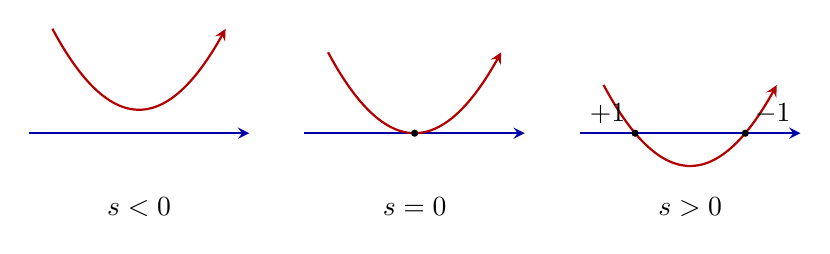
\begin{tikzpicture}[x=1cm,y=0.85cm,>=stealth]
	\begin{scope}
		\draw[->,blue!65!black,thick] (-1.4,0)--(1.4,0);
		\draw[->,red!70!black,thick,domain=-1.1:1.1,samples=40] plot (\x,{\x*\x+0.35});
		\node at (0,-1.1) {\(s<0\)};
	\end{scope}
	\begin{scope}[xshift=3.5cm]
		\draw[->,blue!65!black,thick] (-1.4,0)--(1.4,0);
		\draw[->,red!70!black,thick,domain=-1.1:1.1,samples=40] plot (\x,{\x*\x});
		\fill (0,0) circle (1.3pt);
		\node at (0,-1.1) {\(s=0\)};
	\end{scope}
	\begin{scope}[xshift=7cm]
		\draw[->,blue!65!black,thick] (-1.4,0)--(1.4,0);
		\draw[->,red!70!black,thick,domain=-1.1:1.1,samples=40] plot (\x,{\x*\x-0.49});
		\fill (-0.7,0) circle (1.3pt) node[above left] {\(+1\)};
		\fill (0.7,0) circle (1.3pt) node[above right] {\(-1\)};
		\node at (0,-1.1) {\(s>0\)};
	\end{scope}
\end{tikzpicture}

	\caption{相切附近的交点生成。曲线按横坐标递增定向，横轴向右定向；出现的两个交点分别贡献 \(+1\) 和 \(-1\)。}
	\label{g2:fig:intersection-pair}
\end{figure}

\subsection{一参数族给出的配边}
\label{g2:subsec:1602:03}

第14章已经将同伦横截化，得到连接端点逆像的紧流形。现在给这个配边定向，就能把模二不变性加强为整数不变性。这里需要核对时间方向与法方向的排列，而不只是指出端点成对出现。

\begin{theorem}\label{g2:thm:intersection-homotopy-invariance}
	设 \(M\) 是已定向、无边界的光滑 \(n\) 维流形，\(B\subset M\) 是已定向、闭的无边界嵌入 \(q\) 维子流形，\(X\) 是紧、已定向、无边界的光滑 \(p\) 维流形，\(p+q=n\)。若光滑映射 \(f_0,f_1:X\to M\) 横截于 \(B\) 且连续同伦，则
	\[
		I(f_0,B)=I(f_1,B).
	\]
\end{theorem}
\begin{proof}
	由\cref{g2:thm:transverse-homotopy-cobordism}，可选横截同伦 \(H:X\times[0,1]\to M\)，在两个端点的时间邻域中分别等于 \(f_0,f_1\)。其逆像 \(W=H^{-1}(B)\) 是紧一维带边界流形，边界是两端逆像的不交并。这里 \(X\) 紧、\(B\) 闭保证 \(W\) 紧。

	给 \(X\times[0,1]\) 取先 \(\mathrm{T}X\)、后 \(\partial_t\) 的乘积定向。商微分给出短正合列
	\[
		0\longrightarrow\mathrm{T}W\longrightarrow\mathrm{T}(X\times[0,1])|_W
		\xrightarrow{\ \overline{\mathrm{d}H}\ }H^*\nu B\longrightarrow0.
	\]
	规定 \(W\) 的正向，使法方向排在 \(W\) 的切方向之前，即 \((H^*\nu B,\mathrm{T}W)\) 给出源乘积的定向。更具体地，先列法基的提升，最后列 \(W\) 的正向切向量。

	在端点邻域，\(H\) 与时间无关。若 \(x\in f_i^{-1}(B)\)，记其局部符号为 \(\varepsilon_x\)。法基在 \(\mathrm{T}_xX\) 中的提升相对于 \(X\) 定向具有符号 \(\varepsilon_x\)，故上述规则使 \(W\) 的正向切向量为 \(\varepsilon_x\partial_t\)。采用外法向优先的边界定向，\(t=1\) 端点的符号是 \(\varepsilon_x\)，\(t=0\) 端点的符号是 \(-\varepsilon_x\)。因此
	\[
		\sum_{z\in\partial W}\varepsilon_z=I(f_1,B)-I(f_0,B).
	\]
	紧一维有向流形的边界符号之和为零：按第14章证明中的有限坐标弧分割，把各小弧沿定向排列，每条小弧贡献“终点减起点”，内部端点两两抵消，剩下的就是边界端点。于是右端为零。
\end{proof}

由此可对任意光滑 \(f:X\to M\) 选一个横截扰动 \(f'\)，定义 \(I(f,B)=I(f',B)\)。两个这样的扰动均与 \(f\) 同伦，定理保证良定义。对紧嵌入 \(A\) 使用上一小节的环境扰动，便定义 \(I_M(A,B)\)。其交换及反向规则仍成立：先把两片置于横截位置，再应用\cref{g2:prop:intersection-linear-signs}；更换所移动的一片也不影响结果，因为保持定向的环境微分同胚满足 \(I(A,\Phi(B))=I(\Phi^{-1}(A),B)\)，而 \(\Phi^{-1}|_A\) 与包含映射同伦。

\ProseParagraphBreak

紧性可以用“整个交点轨迹紧”替代，但不能只要求每张切片有有限个交点。例如 \(f_t:\mathbb R\to\mathbb R\)、\(f_t(x)=tx-1\)，以正向原点作为 \(B\)。\(t=0\) 时无交点，\(t>0\) 时恰有一个符号为正的交点 \(x=1/t\)。当 \(t\downarrow0\) 时它逃向无穷，轨迹不是紧配边，所以整数计数发生变化。这个例子说明，在非紧源上应用配边证明时，必须控制整条同伦的逆像。

\subsection{交数与帽积配对的比较}
\label{g2:subsec:1602:04}

以下设环境 \(M\) 闭且已定向，以便使用整数基本类 \([M]\)。\cref{g2:cor:closed-poincare-duality}给出同构
\[
	D_M:H^k(M;\mathbb Z)\longrightarrow H_{n-k}(M;\mathbb Z),\qquad
	D_M(\alpha)=\alpha\frown[M].
\]
对闭已定向嵌入子流形 \(i_B:B^q\hookrightarrow M\)，记
\[
	\mathrm{PD}_M(B)=D_M^{-1}\bigl((i_B)_*[B]\bigr)\in H^{n-q}(M;\mathbb Z).
\]
这里的 \(\mathrm{PD}\) 是 Poincaré 对偶类；它由帽积定义。要证明它检测穿过 \(B\) 的次数，需在 \(B\) 附近找到一个具体相对类，并核对其帽积正好留下 \(B\) 的基本类。

\begin{lemma}\label{g2:lem:normal-relative-class}
	设 \(M\) 是闭、已定向的光滑 \(n\) 维流形，\(B\subset M\) 是闭、已定向的嵌入 \(q\) 维子流形，\(p=n-q\)。法丛采用\eqref{g2:eq:normal-first-orientation}的定向。存在唯一的类
	\[
		u_B\in H^p(M,M\setminus B;\mathbb Z),
	\]
	使它在每个小法向 \(p\) 维盘上的限制，在正向局部基本类上取值 \(1\)。若 \(\overline u_B\) 是它在绝对上同调中的像，则
	\begin{equation}\label{g2:eq:normal-class-cap-fundamental}
		\overline u_B\frown[M]=(i_B)_*[B],\qquad
		\overline u_B=\mathrm{PD}_M(B).
	\end{equation}
\end{lemma}
\begin{proof}
	由\cref{g2:thm:tubular-neighborhood}，可将 \(B\) 的一个开邻域 \(U\) 识别为法丛的一个开圆盘丛；沿纤维径向重参数化，它与整个法丛 \(E\) 微分同胚，并保持零截面及纤维定向。\cref{g2:prop:relative-cohomology-exactness}的切除把 \(H^p(M,M\setminus B)\) 识别为 \(H^p(E,E\setminus B)\)。因此先在法丛中构造相对类。

	对任一法丛可平凡化的开集 \(V\subset B\)，选保持法向定向的平凡化，得到空间对
	\[
		(E|_V,E|_V\setminus V)\cong
		(\mathbb R^p\times V,(\mathbb R^p\setminus\{0\})\times V).
	\]
	相对 Eilenberg--Zilber 比较给出
	\begin{equation}\label{g2:eq:normal-low-degree-local}
		H^j(E|_V,E|_V\setminus V;\mathbb Z)\cong H^{j-p}(V;\mathbb Z).
	\end{equation}
	恢复这一计算的理由：\cref{g2:prop:cross-cup-evaluation}证明中的相对链比较将左侧链模型写成 \(C_*(\mathbb R^p,\mathbb R^p\setminus\{0\})\otimes C_*(V)\)。第一因子的同调只在 \(p\) 次为 \(\mathbb Z\)；由\cref{g2:lem:free-complex-splitting}，其圈边界序列可分裂为一个 \(\mathbb Z\) 加若干两项可缩复形，故它链同伦等价于仅在 \(p\) 次有 \(\mathbb Z\) 的复形。张量后再取 \(\operatorname{Hom}(-,\mathbb Z)\)，便得到上同调的次数平移。特别地，\(j<p\) 时左侧为零，\(j=p\) 时它由每个分支上的纤维取值唯一确定；全部取值为 \(1\) 的类就是正向纤维生成元与 \(1\in H^0(V)\) 的外积。

	这些局部类可以唯一粘合。取覆盖紧流形 \(B\) 的有限个丛平凡化开集，逐个取并。对两个开集 \(V,W\)，相对 Mayer--Vietoris 列包含
	\[
		H^{p-1}(E|_{V\cap W},E|_{V\cap W}\setminus(V\cap W))
		\longrightarrow H^p(E|_{V\cup W},E|_{V\cup W}\setminus(V\cup W))
	\]
	及其后的“限制到 \(V,W\)，再取交集上的差”两条箭头。这条列由相对小链模型的短正合列取对偶得到，和第6章使用的相对 Mayer--Vietoris 构造相同。归纳时，交集位于新加入的平凡化开集中，故\eqref{g2:eq:normal-low-degree-local}适用。其 \(p-1\) 次群为零，且两侧的 \(p\) 次局部类在交集上都以每根正向纤维的取值 \(1\) 为特征，所以差为零。正合性给出延拓的存在与唯一性。相同正合列也保持低于 \(p\) 次的消失，完成归纳。于是得到 \(u_B\)。改变管状邻域或平凡化后，纤维的局部取值不变，唯一性保证所取的是同一相对类。

	接着计算帽积。把 \(u_B\) 切除到 \(U\)，记作 \(u\)。\cref{g2:prop:relative-cap}给出
	\[
		z_U=u\frown[U]_B\in H_q(U;\mathbb Z),
	\]
	其中 \([U]_B\in H_n(U,U\setminus B;\mathbb Z)\) 是第6章的紧集基本类。令 \(r:U\to B\) 为管状收缩。要证明 \(r_*z_U=[B]\)，依\cref{g2:lem:compact-localization}，只需在每个 \(b\in B\) 核对其顶次局部值。

	在 \(b\) 附近选法向优先的乘积坐标 \((z,y)\in\mathbb R^p\times\mathbb R^q\)，其中 \(B\) 为 \(z=0\)。令 \(v_b\in H^q(B,B\setminus\{b\};\mathbb Z)\) 为在 \(B\) 的正向局部基本类上取值 \(1\) 的类。相对帽积的自然性及\eqref{g2:eq:cap-evaluation}在小链模型中的同一计算给出
	\begin{equation}\label{g2:eq:normal-cap-local-test}
		\left\langle v_b,\operatorname{loc}_b(r_*z_U)\right\rangle
		=\left\langle u\smile r^*v_b,[U]_{\{b\}}\right\rangle=1.
	\end{equation}
	说明这里的支集对应：\(u\) 的相对支集为 \(B\)，\(r^*v_b\) 的相对支集为法纤维 \(r^{-1}(b)\)，两者相交于 \(b\)。所以其相对杯积在 \(H^n(U,U\setminus\{b\})\) 中；局部化的基本类正是 \([U]_{\{b\}}\)。最后一个等号是\cref{g2:prop:local-cross-normalization}：先法向、后基底的两个正向局部生成元之积，在环境正向基本类上取值 \(1\)。某个因子为零维时，该计算退为点上乘法，结论相同。

	因此 \(r_*z_U\) 在每点的局部值都与 \([B]\) 相同，基本类的唯一性给出等式。将紧支相对类映入 \(M\)，帽积自然性又给出
	\[
		\overline u_B\frown[M]=(i_U)_*z_U
		=(i_B)_*r_*z_U=(i_B)_*[B].
	\]
	中间等式使用管状邻域沿纤维缩放到零截面的形变收缩。最后由 \(D_M\) 的单射性，\(\overline u_B=\mathrm{PD}_M(B)\)。
\end{proof}

这个相对类把“穿过 \(B\)”变成一个可以拉回的代数条件。法向小盘上的归一化决定每次横穿的贡献，上一证明中的帽积计算则保证它与第6章已经采用的对偶约定一致。

\begin{theorem}[几何相交与对偶配对]\label{g2:thm:geometric-intersection-pairing}
	设 \(M\) 是闭、已定向的光滑 \(n\) 维流形，\(B\subset M\) 是闭、已定向的嵌入 \(q\) 维子流形，\(X\) 是闭、已定向的光滑 \(p\) 维流形，\(p+q=n\)。若光滑映射 \(f:X\to M\) 横截于 \(B\)，且法丛采用法向优先定向，则
	\[
		\sum_{x\in f^{-1}(B)}\varepsilon_x(f,B)
		=\left\langle f^*\mathrm{PD}_M(B),[X]\right\rangle.
	\]
	对任意光滑 \(f\)，左侧采用横截扰动所定义的 \(I(f,B)\) 后，等式仍成立。特别地，若 \(A^p\subset M\) 也是闭已定向嵌入子流形，记 \([A]\)、\([B]\) 为其基本类在 \(M\) 中的推前，则
	\begin{equation}\label{g2:eq:intersection-cup-pairing}
		I_M(A,B)=\langle\mathrm{PD}_M(B),[A]\rangle
		=\langle\mathrm{PD}_M(A)\smile\mathrm{PD}_M(B),[M]\rangle.
	\end{equation}
\end{theorem}
\begin{proof}
	令 \(Z=f^{-1}(B)\)。它是有限点集。上一引理的相对类拉回为
	\[
		f^*u_B\in H^p(X,X\setminus Z;\mathbb Z).
	\]
	基本类的局部化与相对配对自然性给出
	\[
		\left\langle f^*\mathrm{PD}_M(B),[X]\right\rangle
		=\langle f^*u_B,[X]_Z\rangle
		=\sum_{x\in Z}\left\langle(f^*u_B)_x,[X]_x\right\rangle.
	\]
	最后一步在 \(Z\) 的互不相交小坐标邻域中切除；基本类限制到每点都为该点的正向局部类，所以有限直和中的每项系数都是 \(1\)。

	对 \(x\in Z\)，取 \(f(x)\) 附近的法向坐标 \(z:M\supset U\to\mathbb R^p\)。法向部分 \(z\circ f\) 在 \(x\) 的微分是定义 \(\varepsilon_x(f,B)\) 的线性同构。由逆函数定理，它在小邻域内为局部微分同胚，按其行列式符号将 \([X]_x\) 送到正向法盘基本类或其相反数。\(u_B\) 在这个正向法盘上取值 \(1\)，故每项恰等于 \(\varepsilon_x(f,B)\)。这证明横截情形。

	一般 \(f\) 的横截扰动 \(f'\) 与 \(f\) 同伦，所以它们诱导相同的上同调拉回；左侧按此前的不变性定义，等式随之成立。取 \(f=i_A\)，得到\eqref{g2:eq:intersection-cup-pairing}的第一个等式。第二个等式由帽积顺序决定：
	\[
		\begin{aligned}
		\langle\mathrm{PD}_M(B),[A]\rangle
		&=\langle\mathrm{PD}_M(B),\mathrm{PD}_M(A)\frown[M]\rangle\\
		&=\langle\mathrm{PD}_M(A)\smile\mathrm{PD}_M(B),[M]\rangle,
		\end{aligned}
	\]
	最后一行正是\eqref{g2:eq:cap-evaluation}。因此此处杯积先放 \(A\) 的对偶类，再放 \(B\) 的对偶类。
\end{proof}

\begin{corollary}\label{g2:cor:intersection-homological-invariance}
	闭已定向光滑 \(n\) 维流形中的互补维闭已定向嵌入子流形，其相交数只依赖整数同调类。它是这些类的双线性配对；若任一类为挠类，则相交数为零。交换两类乘以 \((-1)^{pq}\)，反转任一子流形或环境的定向均使相交数反号。
\end{corollary}
\begin{proof}
	\(D_M^{-1}\)、杯积及基本类取值均线性，所以\eqref{g2:eq:intersection-cup-pairing}只依赖同调类且双线性。若 \(r[A]=0\)，则 \(rI_M(A,B)=0\)，而整数群无挠，故 \(I_M(A,B)=0\)，另一因子同理。对偶类次数分别为 \(q,p\)，分次交换律给出 \((-1)^{pq}\)。子流形反向使其基本类及对偶类反号；环境反向使 \([M]\) 与 \(D_M\) 都反号，因此两个对偶类各反号，最终的基本类取值再反号，总变化仍为负号。
\end{proof}

\begin{example}\label{g2:exm:torus-poincare-sign-check}
	回到环面中的 \(a,b\)。令 \(\xi,\eta\in H^1(T^2;\mathbb Z)\) 分别从第一、第二圆周拉回正向生成元，则 \(\langle\xi\smile\eta,[T^2]\rangle=1\)。由帽积取值公式，\(D(\xi)=[b]\)、\(D(\eta)=-[a]\)，故
	\[
		\mathrm{PD}(a)=-\eta,\qquad \mathrm{PD}(b)=\xi,\qquad
		\langle(-\eta)\smile\xi,[T^2]\rangle=1.
	\]
	这与两条正向曲线的实际交点符号相同，也说明法向优先约定中的负号如何与杯积交换符号配合。
\end{example}

式\eqref{g2:eq:intersection-cup-pairing}也对任意互补维同调类定义代数相交配对；当类已有光滑子流形代表时，定理将它解释为横截交点数。以 \(\mathbb F_2\) 为系数时，同样的局部类、粘合与帽积证明给出模二相交配对：局部生成元没有正负之分，因而不需要环境及两片的整数定向。

% !TeX root = ../../Book2.tex
% 纲要标题：### 16.3 向量场零点指标
% 纲要位置：几何学计划纲要.md，第 1589 行。
% 正文状态：未撰写；本文件目前是框架。

% 纲要内容开始
% 
% * 局部球面映射度
% * 非退化零点的行列式符号
% * 局部扰动与指标可加性
% * Euler 类的后续解释
% 
% 纲要内容结束

\section{向量场零点指标}
\label{g2:sec:1603}

待撰写

\subsection{局部球面映射度}
\label{g2:subsec:1603:01}
待撰写

\subsection{非退化零点的行列式符号}
\label{g2:subsec:1603:02}
待撰写

\subsection{局部扰动与指标可加性}
\label{g2:subsec:1603:03}
待撰写

\subsection{Euler 类的后续解释}
\label{g2:subsec:1603:04}
待撰写
% 纲要条目排为编号小节标题，并进入目录与书签；说明段仍保留于纲要注释中。

% !TeX root = ../../Book2.tex
% 纲要标题：### 16.4 不动点与 Lefschetz 公式
% 纲要位置：几何学计划纲要.md，第 1646 行。
% 正文状态：未撰写；本文件目前是框架。

% 纲要内容开始
% 
% * 图像和对角线
% * 横截不动点的局部指数
% * 对角类和上同调迹
% * Lefschetz 数非零的存在推论
% 
% ---
% 
% 纲要内容结束

\section{不动点与 Lefschetz 公式}
\label{g2:sec:1604}

待撰写

\subsection{图像和对角线}
\label{g2:subsec:1604:01}
待撰写

\subsection{横截不动点的局部指数}
\label{g2:subsec:1604:02}
待撰写

\subsection{对角类和上同调迹}
\label{g2:subsec:1604:03}
待撰写

\subsection{Lefschetz 数非零的存在推论}
\label{g2:subsec:1604:04}
待撰写
% 纲要条目排为编号小节标题，并进入目录与书签；说明段仍保留于纲要注释中。


\begin{chaptersummary}
	映射度将每个正则原像的微分符号相加，所得整数既是推前基本类的倍数，也是拉回顶次形式的积分倍数。非紧源上，局部有限基本类和紧支形式承担相同的比较，而固有映射与整体固有同伦保证支集和无穷远处的控制。相交数用法向优先定向比较源切空间与目标法空间；横截扰动给出有限计数，有向一维配边保证它不依赖扰动，局部法向类进一步把它识别为帽积配对。

	\ProseParagraphBreak

	向量场的孤立零点由小球边界的方向度赋予指标，非退化时为线性化行列式的符号。保持边界无零的扰动只能重新分配内部指标，不能改变总和；闭流形上的截面同伦也保持总指标，即使流形不可定向。对于不动点，图像与对角线把同一局部度变成 \(\operatorname{sgn}\det(I-\mathrm{d}f_x)\)，对角类的杯积计算再把局部指数和化为 Lefschetz 数。非零总量迫使相应原像、交点或不动点存在，而总量为零仍可能有彼此抵消的局部贡献。
\end{chaptersummary}

\BookExercises

\begin{exercise}\label{g2:ex:degree-sublinear-perturbation}
	设 \(A\in\operatorname{GL}(n,\mathbb R)\)，\(r:\mathbb R^n\to\mathbb R^n\) 光滑，且 \(|r(x)|/|x|\to0\) 当 \(|x|\to\infty\)。证明 \(F(x)=Ax+r(x)\) 固有，计算其度，并证明 \(F\) 满射。若目标正则值的全部原像点处均有 \(\det\mathrm{D}F>0\)，这些原像点的数量有何限制？
\end{exercise}
\begin{solution}
	选 \(c>0\) 使 \(|Ax|\ge c|x|\)。在某个大球之外有 \(|r(x)|\le c|x|/2\)，所以同伦 \(H(x,t)=Ax+t r(x)\) 对所有 \(0\le t\le1\) 同时满足
	\[
		|H(x,t)|\ge c|x|/2.
	\]
	目标紧集有界，因而其在 \(H\) 下的原像包含于一个固定闭球与 \([0,1]\) 的乘积；该原像又闭，所以紧。因此 \(H\) 是整体固有同伦，特别 \(F\) 固有，且
	\[
		\deg F=\deg A=\operatorname{sgn}\det A\ne0.
	\]
	非零度给出满射性。若某正则值的全部原像符号为正，符号和就是原像点数。因原像非空，该数必须为1，同时迫使 \(\det A>0\)。若 \(\det A<0\)，任何正则值的原像都必须至少包含一个反向点。
\end{solution}

\begin{exercise}\label{g2:ex:proper-local-diffeomorphism-degree}
	设 \(f:M^n\to N^n\) 为连通定向无边界光滑流形间的固有光滑映射，\(n\ge1\)，且 \(\mathrm{d}f\) 处处可逆。证明 \(f\) 满射，所有纤维有同一个有限正基数 \(r\)，并有 \(|\deg f|=r\)。若某个纤维只有一个点，证明 \(f\) 为微分同胚。将此结论用于上一题：若 \(\det\mathrm{D}F\) 处处非零，可以得到什么加强？
\end{exercise}
\begin{solution}
	微分的定向符号是 \(M\) 上连续取值于 \(\{1,-1\}\) 的函数，因连通性而恒等于某个 \(\varepsilon\)。任取 \(x_0\in M\)，\(y_0=f(x_0)\) 是正则值，紧离散纤维有有限个 \(r_0\ge1\) 点。因此 \(\deg f=\varepsilon r_0\ne0\)，从而 \(f\) 满射。所有目标点都是正则值，再次使用求和公式，得到
	\[
		\deg f=\varepsilon\#f^{-1}(y),
	\]
	所以每个纤维都有 \(r_0=|\deg f|\) 个点。若某个纤维单点，则全部纤维单点，\(f\) 双射。它的局部逆由逆函数定理光滑；各局部逆在交叠处因单射性一致，故拼成光滑整体逆。

	上一题已给出 \(|\deg F|=1\)，因此若 \(\mathrm{D}F\) 处处可逆，\(F:\mathbb R^n\to\mathbb R^n\) 就是整体微分同胚。这里无穷远处的增长控制与局部微分可逆分别保证固有性与局部逆，两者合起来才得到整体逆。
\end{solution}

\begin{exercise}\label{g2:ex:real-polynomial-degree}
	设 \(p(x)=a_mx^m+\cdots+a_0\) 是非常数实多项式，\(a_m\ne0\)。把实线取标准定向，按 \(m\) 的奇偶性及 \(a_m\) 的符号计算 \(\deg p\)。由此证明：对任意正则值 \(y\)，方程 \(p(x)=y\) 的实根数与 \(m\) 模2同余。证明中须核对所用同伦的整体固有性。
\end{exercise}
\begin{solution}
	令 \(q(x)=p(x)-a_mx^m\)，取同伦 \(H(x,t)=a_mx^m+tq(x)\)。因 \(\deg q<m\)，充分大 \(|x|\) 时有 \(|q(x)|\le|a_m||x|^m/2\)，故
	\[
		|H(x,t)|\ge |a_m||x|^m/2
	\]
	对所有 \(t\in[0,1]\) 同时成立。与上一题同理，\(H\) 整体固有，因而 \(\deg p=\deg(x\mapsto a_mx^m)\)。

	若 \(m\) 为奇数，任取非零目标值，有唯一实原像，导数 \(ma_mx^{m-1}\) 的符号为 \(\operatorname{sgn}a_m\)，故度为该符号。若 \(m\) 为偶数，取与 \(a_m\) 异号的目标值，原像为空，故度为0。等价地，同号非零目标值的两个原像导数符号相反，仍给出0。

	正则值的所有实原像都是单根，且有限。模2后每个 \(\pm1\) 都等于1，所以
	\[
		\#p^{-1}(y)\equiv\deg p\equiv m\pmod2.
	\]
	这既给出奇次多项式至少有一个实根，也说明偶次情形的正则实根总数为偶数。
\end{solution}

\begin{exercise}\label{g2:ex:boundary-degree-balance}
	设 \(W^{n+1}\) 为紧定向光滑带边界流形，\(n\ge1\)，边界的连通分支为 \(M_1,\ldots,M_s\)，均取外法向优先定向。设 \(N^n\) 为连通闭定向光滑流形，\(F:W\to N\) 光滑，记 \(f_j=F|_{M_j}\)。证明
	\[
		\sum_{j=1}^s\deg f_j=0.
	\]
	把结论用于圆环 \(W=\{z\in\mathbb C:1\le|z|\le2\}\)：若把内、外两个边界圆都按逆时针方向参数化，它们到 \(S^1\) 的限制映射度是什么关系？
\end{exercise}
\begin{solution}
	取 \(N\) 上积分为1的光滑顶次形式 \(\eta\)。因为 \(\mathrm{d}\eta=0\)，第一卷的 Stokes 定理和\cref{g2:thm:degree-comparison}给出
	\[
		\sum_j\deg f_j
		=\sum_j\int_{M_j}f_j^*\eta
		=\int_{\partial W}F^*\eta
		=\int_W\mathrm{d}(F^*\eta)=0.
	\]
	关键是所有边界分支使用诱导定向。对平面标准定向的圆环，外边界的诱导方向为逆时针，内边界为顺时针。因此若两个参数圆都取逆时针方向，内边界度要在上述和式中另乘 \(-1\)。公式成为 \(\deg f_{\mathrm{out}}-\deg f_{\mathrm{in}}=0\)，即二者的度相等。单边界情形的延拓障碍可对照\cite[第459页，定理17.38]{Lee2012Smooth}。
\end{solution}

% 第16.2节习题候选，题目及解答供并入章末。
\begin{exercise}\label{g2:ex:torus-slope-intersection}
	给 \(T^2=\mathbb R^2/\mathbb Z^2\) 取标准定向。设 \((r,s),(u,v)\in\mathbb Z^2\) 均为非零本原向量，令 \(A(t)=(rt,st)\)、\(B(t)=(ut,vt)\)，参数 \(t\) 模 \(1\)，并以递增参数定向。证明这两条曲线为嵌入圆周，且 \(I(A,B)=rv-su\)。当 \(rv-su\ne0\) 时求实际交点数；当 \(rv-su=0\) 时给出不交的微小扰动。
\end{exercise}
\begin{solution}
	若 \(A(t)=A(t')\)，则 \(r(t-t'),s(t-t')\in\mathbb Z\)。由 Bézout 等式及 \(\gcd(r,s)=1\)，得 \(t-t'\in\mathbb Z\)，故 \(A\) 单射；其导数不为零，源紧，所以为嵌入，\(B\) 同理。记标准坐标圆周类为 \(a,b\)，则 \([A]=ra+sb\)、\([B]=ua+vb\)。正文已算出 \(I(a,b)=1\)、\(I(b,a)=-1\)；平移一个坐标圆周得到与原圆周不交的同调代表，所以 \(I(a,a)=I(b,b)=0\)。双线性给出 \(I(A,B)=rv-su\)。

	还可直接数交点。取整数矩阵 \(P\in\operatorname{SL}(2,\mathbb Z)\)，使 \(P(r,s)^{\mathsf T}=(1,0)^{\mathsf T}\)；它由 Bézout 等式构造，并诱导保持定向的环面微分同胚。记 \(P(u,v)^{\mathsf T}=(u',v')^{\mathsf T}\)，则 \(v'=rv-su\)。\(B\) 与水平圆周相交恰要求 \(v't\in\mathbb Z\)。若 \(v'\ne0\)，模 \(1\) 恰有 \(|v'|\) 个参数；\(B\) 嵌入，给出相同数量的不同交点。各点的有序切向量行列式均为 \(v'\)，所以全部具有符号 \(\operatorname{sgn}(v')\)。若 \(v'=0\)，本原性使 \(u'=\pm1\)，两曲线的像都是水平圆周；将其中一条平移到 \(y=\varepsilon\ne0\) 即不相交，再用 \(P^{-1}\) 送回即可。
\end{solution}

\begin{exercise}\label{g2:ex:product-sphere-self-intersection}
	给 \(S^2\times S^2\) 取先第一因子、后第二因子的乘积定向。令 \(A=S^2\times\{y_0\}\)、\(B=\{x_0\}\times S^2\)，分别取因子定向。计算它们的全部相交配对。若闭已定向嵌入曲面 \(\Sigma\subset S^2\times S^2\) 满足 \([\Sigma]=m[A]+n[B]\)，求 \(I(\Sigma,\Sigma)\)，并说明 \(mn\ne0\) 时为何任何与 \(\Sigma\) 同调的嵌入曲面都不能与它不交。
\end{exercise}
\begin{solution}
	两片在 \((x_0,y_0)\) 唯一相交，先列 \(A\) 的正向基、再列 \(B\) 的正向基，正好是乘积正向基，所以 \(I(A,B)=1\)。两片维数均为 \(2\)，交换符号为 \((-1)^4=1\)，故 \(I(B,A)=1\)。把 \(y_0\) 移到另一点，得到与 \(A\) 同调且不交的纤维，故 \(I(A,A)=0\)；同理 \(I(B,B)=0\)。于是交矩阵为
	\[
		\begin{pmatrix}0&1\\1&0\end{pmatrix},\qquad
		I(\Sigma,\Sigma)=2mn.
	\]
	如果 \(\Sigma'\) 与 \(\Sigma\) 同调且二者不交，则 \(I(\Sigma,\Sigma')=0\)。同调不变性却使该数等于 \(2mn\)，所以 \(mn\ne0\) 时不可能。这里的自交数按两份代表作横截扰动计算，并非把 \(\Sigma\cap\Sigma\) 当成有限点集。
\end{solution}

\begin{exercise}\label{g2:ex:intersection-boundary-sign}
	设 \(M^n\) 是已定向无边界光滑流形，\(C^{p+1}\subset M\) 是紧已定向带边界嵌入子流形，\(A=\partial C\) 采用外法向优先的边界定向，\(B^q\subset M\) 是已定向闭嵌入无边界子流形，\(p+q=n\)。假设 \(C\) 及 \(A\) 都与 \(B\) 横截。用一维交集 \(W=C\cap B\) 证明 \(I(A,B)=0\)，并计算 \(\partial W\) 的点符号与 \(\varepsilon_z(A,B)\) 的关系，其中 \(W\) 按 \((\nu B,\mathrm{T}W)=\mathrm{T}C\) 定向。
\end{exercise}
\begin{solution}
	带边界横截逆像定理给出紧一维流形 \(W\)，并有 \(\partial W=A\cap B\)。设 \(z\) 为边界交点，\(a_1,\ldots,a_p\) 是 \(A\) 的正向基，\(o\) 是 \(C\) 的向外方向，则 \((o,a_1,\ldots,a_p)\) 给出 \(C\) 的正向。因为 \(A\pitchfork B\)，法基可在 \(\mathrm{T}A\) 内提升；其相对于 \((a_1,\ldots,a_p)\) 的符号为 \(\varepsilon_z(A,B)\)。

	把 \(o\) 从这些法基提升之后移到之前，需要交换 \(p\) 次。因而将 \(W\) 的正向与它的向外方向比较，得到
	\[
		\varepsilon_z(\partial W)=(-1)^p\varepsilon_z(A,B).
	\]
	向外向量为使其切于 \(W\) 而添加的切向分量，不改变这一行列式符号。紧一维有向流形的边界符号之和为零，故
	\[
		0=\sum_{z\in\partial W}\varepsilon_z(\partial W)=(-1)^pI(A,B),
	\]
	即 \(I(A,B)=0\)。
\end{solution}

\begin{exercise}\label{g2:ex:projective-lines-mod-two-intersection}
	在 \(\mathbb RP^2\) 中取两条不同的射影直线 \(L_0,L_1\)。证明它们横截相交于一点，模二相交数为 \(1\)，因而与它们分别模二同调的两个嵌入圆周不能不交。解释为何不能在本例中直接使用本节的整数有向相交配对。
\end{exercise}
\begin{solution}
	射影直线来自 \(\mathbb R^3\) 中的二维线性子空间。两个不同二维子空间的交恰为一维，所以对应的射影直线只有一个交点。作线性坐标变换后，可设它们分别为 \(z_2=0\) 和 \(z_1=0\)，交点为 \([1:0:0]\)。在仿射图 \(z_0\ne0\) 中，两条直线是两个坐标轴，故横截。模二计数因此为 \(1\)。

	本节模二版本的几何相交与对偶配对说明该数只依赖模二同调类。若两条相应代表不交，计数就为 \(0\)，与 \(1\) 矛盾。\(\mathbb RP^2\) 不可定向，且直线的法线丛也是不可定向的：把一条直线提升为 \(S^2\) 上的赤道，沿赤道的一个固定向北法向量在对径识别下被微分送到相反方向，绕投影圆周一周后法向反转。因此本例不能连续选择整数局部符号所需的法向定向，而模二计数不受反号影响。
\end{solution}

\begin{exercise}\label{g2:ex:mixed-monomial-vector-index}
	在标准平面切标架中，把向量场的系数写成复数。设它在原点附近满足
	\[
		F(z)=z^p\overline z^{\,q}+r(z),\qquad r(z)=o(|z|^{p+q}),
	\]
	其中 \(p,q\ge0\)、\(p+q\ge1\)，且 \(F\) 光滑。证明原点是孤立零点，指标为 \(p-q\)。在充分小的闭圆盘内，将该场作一个在边界上充分小的扰动，假设新场全部零点非退化。证明新零点总数 \(N\) 满足
	\[
		N\ge|p-q|,\qquad N\equiv p-q\pmod2.
	\]
\end{exercise}
\begin{solution}
	令 \(d=p+q\)。充分小的 \(|z|>0\) 时，\(|r(z)|<|z|^d/2\)，而 \(|z^p\overline z^{\,q}|=|z|^d\)，所以 \(|F(z)|>|z|^d/2>0\)。同时 \(F(0)=0\)，故原点孤立。对 \(0\le s\le1\)，\(z^p\overline z^{\,q}+s r(z)\) 在这个穿孔邻域内都非零。边界归一化因此把 \(F\) 同伦到主项；在 \(z=\varepsilon e^{\mathrm i\theta}\) 上，主项的单位方向为 \(e^{\mathrm i(p-q)\theta}\)。圆周映射度于是给出 \(\operatorname{ind}_0(F)=p-q\)。

	固定上述小圆盘 \(D\)，记 \(c=\min_{\partial D}|F|>0\)。若扰动 \(G\) 满足 \(\sup_{\partial D}|G-F|<c\)，则 \((1-s)F+sG\) 在边界始终非零。新零点集闭且不碰边界，非退化性又使它离散，故有限。记正、负指标零点数为 \(N_+,N_-\)。由\cref{g2:thm:local-index-additivity,g2:prop:nondegenerate-vector-index}，
	\[
		N_+-N_-=p-q,\qquad N=N_++N_-.
	\]
	因此 \(N\ge|p-q|\)，且 \(N-(p-q)=2N_-\)，得到奇偶约束。当 \(p=q\) 时原零点仍孤立，但指标为零，结论只要求扰动后的非退化零点成偶数出现，允许全部消失。
\end{solution}

\begin{exercise}\label{g2:ex:product-vector-field-index}
	设 \(X\) 是 \(m\) 维无边界光滑流形 \(M\) 上的向量场，\(Y\) 是 \(n\) 维无边界光滑流形 \(N\) 上的向量场，\(m,n\ge1\)。若 \(a,b\) 分别是其孤立零点，定义乘积场 \(Z(x,y)=(X(x),Y(y))\)。用局部相对同调外积的自然性证明
	\[
		\operatorname{ind}_{(a,b)}Z=\operatorname{ind}_aX\operatorname{ind}_bY.
	\]
	对 \(\mathbb R^3=\mathbb C\times\mathbb R\) 上系数为 \((z^k,-t)\) 的场，\(k\ge1\)，计算原点指标。
\end{exercise}
\begin{solution}
	取把 \(a,b\) 移到零点的坐标，系数分别为 \(F:U\to\mathbb R^m\)、\(G:V\to\mathbb R^n\)，并缩小 \(U,V\)，使每个映射仅在原点为零。乘积系数 \(F\times G\) 在 \(U\times V\) 中也只在 \((0,0)\) 为零，所以乘积零点孤立。

	记正向局部同调生成元为 \(\mu_m,\mu_n\)。第4章相对外积的自然性适用于穿孔开集，因为
	\[
		(U\setminus\{0\})\times V\ \cup\ U\times(V\setminus\{0\})
		=(U\times V)\setminus\{(0,0)\}.
	\]
	\cref{g2:prop:local-cross-normalization}证明中的定向乘积链说明，先列 \(U\) 坐标、再列 \(V\) 坐标时，\(\mu_m\times\mu_n=\mu_{m+n}\)，没有额外符号。于是
	\begin{align*}
		(F\times G)_*(\mu_m\times\mu_n)
		&=F_*\mu_m\times G_*\mu_n\\
		&=(\deg_0F)(\deg_0G)(\mu_m\times\mu_n).
	\end{align*}
	\cref{g2:prop:vector-index-well-defined}已将系数映射的局部同调度识别为向量场指标，因此得到乘法公式。此论证同时适用于退化零点，不要求微分可逆。

	在 \(\mathbb C\) 因子，\(z^k\) 的原点指标为 \(k\)；在实线因子，\(-t\) 的指标为 \(-1\)。采用坐标顺序 \((\operatorname{Re}z,\operatorname{Im}z,t)\)，乘积指标为 \(-k\)。
\end{solution}

\begin{exercise}\label{g2:ex:punctured-rotating-frame-index}
	在穿孔平面圆盘中写 \(z=r e^{\mathrm i\theta}\)，对整数 \(k\) 取由标准标架转动 \(k\theta\) 得到的正向标架
	\[
		e_1=(\cos k\theta,\sin k\theta),\qquad
		e_2=(-\sin k\theta,\cos k\theta).
	\]
	求径向场 \(X(x,y)=(x,y)\) 在这组标架中的系数沿小圆周的绕数。证明当 \(k\ne0\) 时，这组标架不能作为处处非退化的连续标架延过原点，并说明所得系数绕数为什么不违背局部指标的坐标无关性。
\end{exercise}
\begin{solution}
	把平面向量写成复数时，标架变换就是乘以 \(e^{\mathrm ik\theta}\)。若 \(c\) 表示径向场在新标架中的复系数，则 \(e^{\mathrm ik\theta}c=r e^{\mathrm i\theta}\)，所以
	\[
		c=r e^{\mathrm i(1-k)\theta}.
	\]
	沿小圆周归一化后，其绕数为 \(1-k\)。

	若该标架能非退化地连续延过原点，第一列向量 \(e_1\) 就在整个小闭圆盘上连续且非零。将它归一化，可得从闭圆盘到 \(S^1\) 的连续映射，其边界限制为 \(e^{\mathrm i\theta}\mapsto e^{\mathrm ik\theta}\)。把边界圆沿径向缩到圆心，得到这一映射与常值映射的同伦，故边界度必须为0。但它的度为 \(k\)，所以 \(k\ne0\) 时不可能延拓。

	向量场指标要求使用包含零点的坐标图及其坐标切标架。这里 \(k\ne0\) 的标架只存在于穿孔圆盘，零点处缺少这份坐标识别，故不能用其系数绕数代替原点指标。标准标架中的径向场指标仍为1；差出的 \(k\) 正是沿圆周旋转标架自身所贡献的绕数。
\end{solution}

\begin{exercise}\label{g2:ex:odd-dimensional-total-index}
	设 \(X\) 是无边界光滑 \(n\) 维流形上的向量场，\(n\ge1\)，\(p\) 是孤立零点。证明
	\[
		\operatorname{ind}_p(-X)=(-1)^n\operatorname{ind}_pX.
	\]
	再仅用本章的总指标不变性，证明奇数维闭流形上任何只有孤立零点的光滑向量场，其总指标为零；因此它不可能恰有一个零点且该零点非退化。若所有零点都非退化，正、负指标零点数有何关系？
\end{exercise}
\begin{solution}
	在零点附近写 \(X\) 的系数为 \(F\)。负场的单位方向映射为 \(a\circ\widehat F\)，其中 \(a:S^{n-1}\to S^{n-1}\)、\(a(u)=-u\)。\cref{g2:prop:reflection-antipodal-degree}给出 \(\deg a=(-1)^n\)，复合公式遂得所求恒等式。\(n=1\) 时 \(a\) 交换 \(S^0\) 的两点，在约化零次同调上乘以 \(-1\)，同样成立。

	现设 \(M\) 闭且 \(n\) 为奇数。零点集有限，且 \(X,-X\) 有相同零点。记 \(J=\sum_p\operatorname{ind}_pX\)。\cref{g2:thm:total-vector-index-invariance}使 \(-X\) 的总指标也为 \(J\)，而逐点的公式又使它等于 \(-J\)。所以 \(2J=0\)；\(J\) 为整数，故 \(J=0\)。这里不需要整体定向，也没有使用指标总和与 Euler 示性数的比较。

	单个非退化零点的指标为 \(\pm1\)，无法构成总和0，因此题述情形不可能。若所有零点都非退化，设其正、负指标数为 \(N_+,N_-\)，则 \(N_+-N_-=J=0\)，所以两类数量相同，零点总数为偶数。
\end{solution}

\begin{exercise}\label{g2:ex:torus-affine-lefschetz}
	设 \(A\in M_2(\mathbb Z)\)、\(b\in\mathbb R^2\)，令 \(f:\mathbb R^2/\mathbb Z^2\to\mathbb R^2/\mathbb Z^2\) 为 \(f([x])=[Ax+b]\)。计算 \(L(f)\)。若 \(\det(I-A)\ne0\)，证明它恰有 \(|\det(I-A)|\) 个不动点，并计算每点指数。
\end{exercise}
\begin{solution}
	平移 \(b\) 可通过 \(tb\) 同伦移去。一次同调上的矩阵为 \(A\)，一次上同调上的矩阵为 \(A^{\mathsf T}\)；零次作用为恒等，二次作用为乘 \(\det A\)。因此
	\[
		L(f)=1-\operatorname{tr}A+\det A=\det(I-A).
	\]
	记 \(B=I-A\)。不动点方程是 \(Bx\equiv b\pmod{\mathbb Z^2}\)。若 \(\det B\ne0\)，先取 \(x_0=B^{-1}b\)，全部解在环面上形成陪集 \([x_0]+\ker\overline B\)。核为 \(B^{-1}\mathbb Z^2/\mathbb Z^2\)，乘以 \(B\) 将其同构到 \(\mathbb Z^2/B\mathbb Z^2\)。整数 Smith 标准形将后者写成两个有限循环群的直和，其阶为两个非零对角因子的绝对值之积，即 \(|\det B|\)。每点微分均为 \(A\)，故均非退化，指数都等于 \(\operatorname{sgn}\det B\)。指数和为 \(|\det B|\operatorname{sgn}\det B=\det B\)，与 \(L(f)\) 一致。
\end{solution}

\begin{exercise}\label{g2:ex:even-complex-projective-fixed-point}
	设 \(r\geq1\)。利用 \(H^*(\mathbb CP^{2r};\mathbb Z)=\mathbb Z[u]/(u^{2r+1})\)、\(|u|=2\)，证明每个连续映射 \(f:\mathbb CP^{2r}\to\mathbb CP^{2r}\) 都有不动点。\cite[第2.C节，The Lefschetz Fixed Point Theorem]{Hatcher2002}
\end{exercise}
\begin{solution}
	二次整数上同调由 \(u\) 生成，故 \(f^*u=du\)，其中 \(d\in\mathbb Z\)。拉回保持杯积，所以 \(f^*(u^k)=d^ku^k\)。只有偶次上同调非零，故
	\[
		L(f)=1+d+d^2+\cdots+d^{2r}.
	\]
	若 \(d\geq0\)，这个和至少为 \(1\)。若 \(d\leq-1\)，则
	\[
		1+d+\cdots+d^{2r}=\frac{d^{2r+1}-1}{d-1}>0,
	\]
	因为分子、分母同为负数。于是对所有整数 \(d\) 都有 \(L(f)>0\)，由 Lefschetz 不动点定理得到结论。证明使用了杯积将二次作用与所有高偶次作用联系起来，单独知道各次群的秩还不足以得到这些幂次关系。
\end{solution}

\begin{exercise}\label{g2:ex:lefschetz-product}
	设 \(M,N\) 是闭、已定向光滑流形，\(f:M\to M\)、\(g:N\to N\) 连续。证明 \(L(f\times g)=L(f)L(g)\)。如果两映射都光滑且全部不动点非退化，再用局部指数给出同一等式的几何证明。
\end{exercise}
\begin{solution}
	有限维上同调的 Künneth 同构将 \(H^k(M\times N;\mathbb R)\) 写为 \(\bigoplus_{p+q=k}H^p(M;\mathbb R)\otimes H^q(N;\mathbb R)\)。由外积自然性，\((f\times g)^*\) 在对应直和项上为 \(f^*\otimes g^*\)。若两矩阵为 \(A,B\)，则张量基中对角元为 \(A_{ii}B_{jj}\)，所以 \(\operatorname{tr}(A\otimes B)=\operatorname{tr}A\operatorname{tr}B\)。因此
	\[
		L(f\times g)=\sum_{p,q}(-1)^{p+q}\operatorname{tr}(f^*|_{H^p(M)})\operatorname{tr}(g^*|_{H^q(N)})=L(f)L(g).
	\]
	在非退化情形，不动点集为两个有限不动点集的乘积。微分是块对角矩阵，故
	\[
		\operatorname{ind}(f\times g,(x,y))
		=\operatorname{sgn}\det(I-\mathrm{d}f_x)\operatorname{sgn}\det(I-\mathrm{d}g_y).
	\]
	分别对 \(x,y\) 求和，再用 Lefschetz 公式，便得同一等式。
\end{solution}

\begin{exercise}\label{g2:ex:degenerate-circle-fixed-indices}
	固定 \(0<\varepsilon<1/4\)，在 \(S^1=\mathbb R/\mathbb Z\) 上定义 \(f([t])=[t+\varepsilon\sin^2(2\pi t)]\)。求全部不动点及其指数。再考虑 \(f_a([t])=[t+\varepsilon\sin^2(2\pi t)-a]\)：当 \(0<a<\varepsilon\) 时求不动点个数和指数，并说明当 \(-\varepsilon<a<0\) 时发生了什么。
\end{exercise}
\begin{solution}
	\(f\) 的位移增量在 \([0,\varepsilon]\subset[0,1)\) 内，所以不动点恰为 \([0]\)、\([1/2]\)。各点附近的 \(t-f(t)=-\varepsilon\sin^2(2\pi t)\) 在两侧都为负，故由一维局部指数公式，两点指数都为零。所有 \(f_a\) 都同伦于恒等映射，所以 \(L(f_a)=0\)。

	若 \(0<a<\varepsilon\)，位移增量位于 \((-1,1)\)，不动点方程恰为 \(\sin^2(2\pi t)=a/\varepsilon\)。一个周期内有四个解，每个原不动点两侧各有一个。局部位移为 \(h_a(t)=a-\varepsilon\sin^2(2\pi t)\)，其导数
	\[
		h_a'(t)=-4\pi\varepsilon\sin(2\pi t)\cos(2\pi t)
	\]
	在四个解处均非零，符号依次交替；围绕每个原不动点的两个指数分别为 \(+1\)、\(-1\)，故各小邻域内的总指数仍为零。若 \(-\varepsilon<a<0\)，增量 \(\varepsilon\sin^2(2\pi t)-a\) 严格位于 \((0,2\varepsilon)\subset(0,1)\)，没有不动点。原来的两个零指数不动点因此都可在小扰动下消失。
\end{solution}

% !TeX root = ../../Book2.tex
% 纲要标题：## 第17章　Morse 函数、把手与整体拓扑
% 纲要位置：几何学计划纲要.md，第 1655 行。
% 正文状态：未撰写；本文件目前是框架。

% 纲要内容开始
% 
% > 本章目标与证明范围：从非退化临界点的局部二次型，经过次水平集的真实粘合，建立 Morse 不等式与 Poincaré–Hopf。这里不把动态轨线计数当作已经建立的 Morse 同调。
% 
% 纲要内容结束

\chapter{Morse 函数、把手与整体拓扑}
\label{g2:ch:17}
\BookChapterNumber{g2:ch:17}

\begin{chapterabstract}
待撰写
\end{chapterabstract}

\begin{learninggoals}
待撰写
\end{learninggoals}

待撰写

% !TeX root = ../../Book2.tex
% 纲要标题：### 17.1 临界点及 Morse 引理
% 纲要位置：几何学计划纲要.md，第 1659 行。
% 正文状态：初稿；尚未正式审核。

% 纲要内容开始
% 
% * Hessian 的内在定义
% * 非退化标准形的逐变量消去
% * Morse 函数的存在与扰动
% * 相对及带边界数据
% 
% 纲要内容结束

\section{临界点及 Morse 引理}
\label{g2:sec:1701}

把山地浸入逐渐上涨的水中，水面经过普通高度时，岸线只是移动；经过谷底或山口时，水域可能多出一个分支，或把原有分支连接起来。对流形上的函数，决定这种变化的首先是临界点附近的形状。二阶导数给出最容易计算的信息，Morse 引理则说明：在非退化临界点附近，换一套光滑坐标就能把函数精确化成二次型。

\subsection{Hessian 的内在定义}
\label{g2:subsec:1701:01}

设 \(f:M\to\mathbb R\) 光滑。临界点 \(p\) 满足 \(\mathrm df_p=0\)，所以 \(f\) 沿任何方向的一阶变化都为零。要比较不同方向的二阶变化，不能只把某张坐标图里的二阶偏导数矩阵当成天然对象：换坐标时通常会出现额外的一阶导数项。临界点条件恰好使这些项消失。

\begin{proposition}\label{g2:prop:critical-hessian-intrinsic}
	设 \(M\) 为无边界光滑流形，\(f\in C^\infty(M)\)，\(p\) 为 \(f\) 的临界点。对 \(v,w\in\mathrm T_pM\)，任取局部光滑向量场 \(V,W\)，使 \(V_p=v\)、\(W_p=w\)，则
	\[
		\operatorname{Hess}_pf(v,w)\coloneqq V(Wf)(p)
	\]
	与延拓的选择无关，并给出 \(\mathrm T_pM\) 上的对称双线性型。在坐标 \(x^1,\ldots,x^n\) 中，它的矩阵为 \((\partial_i\partial_jf(p))\)。
\end{proposition}
\begin{proof}
	写 \(V=\sum_iV^i\partial_i\)、\(W=\sum_jW^j\partial_j\)。乘积法则给出
	\[
		V(Wf)(p)=\sum_{i,j}V^i(p)\partial_iW^j(p)\partial_jf(p)
		+\sum_{i,j}V^i(p)W^j(p)\partial_i\partial_jf(p).
	\]
	第一项因 \(\mathrm df_p=0\) 为零，第二项只取决于 \(v,w\)，并且对它们双线性。混合偏导数相等又给出对称性。定义左端用向量场作用于函数写成，已经不依赖坐标；右端给出所述矩阵。
\end{proof}

这个双线性型称为 \(f\) 在临界点的\term[Hessianxing]{Hessian 型}[Hessian]。若坐标变换写作 \(x=x(y)\)，则在临界点
\[
	H_y=J^{\mathsf T}H_xJ,\qquad J=\left(\frac{\partial x^i}{\partial y^j}(p)\right).
\]
这是合同变换。因此矩阵的秩及正、负惯性指数有坐标无关的意义；矩阵的具体特征值则随坐标缩放改变。在非临界点，\(f(x)=x\) 经过局部坐标变换 \(y=x+x^2\)，其在原点的二阶导数从 \(0\) 变成 \(-2\)。这说明临界点条件在上述构造中的作用。

\begin{definition}\label{g2:def:morse-critical-point}
	设 \(f\) 为光滑 \(n\) 维流形上的实值光滑函数，\(p\) 为内部临界点。若 \(\operatorname{Hess}_pf\) 非退化，就称 \(p\) 为\term[feituohualinjiedian]{非退化临界点}[nondegenerate critical point]。该型的负惯性指数称为 \(p\) 的\term[Morsezhibiao]{Morse 指标}[Morse index]，记作 \(\lambda(p)\)。无边界流形上的光滑函数若所有临界点都非退化，就称为\term[Morsehanshu]{Morse 函数}[Morse function]。
\end{definition}

指标 \(\lambda(p)\) 等于 Hessian 在其上负定的子空间的最大维数，满足 \(0\le\lambda(p)\le n\)。它计数的是独立的下降方向。\(x^2+y^2\)、\(-x^2+y^2\)、\(-x^2-y^2\) 在原点的指标依次为 \(0,1,2\)。其中鞍点同时有上升和下降方向，不能用“极大或极小”两类描述。

\ProseParagraphBreak

定义允许不同临界点有相同的临界值。例如 \(\cos(2\theta)\) 是圆上的 Morse 函数，却有两个同高的极大点和两个同高的极小点。以后逐个跨越临界值时，会另外使用使临界值互异的扰动。

\subsection{非退化标准形的逐变量消去}
\label{g2:subsec:1701:02}

Taylor 展开把函数写成二次项加高阶余项；对次水平集的粘合来说，精确的标准形更方便，因为可以直接沿坐标方向构造变形。下面的证明将高阶项吸收到坐标中。关键操作仍是配平方，但平方前的系数现在是光滑函数，必须同时检查所得变量确实构成坐标。

\begin{theorem}[Morse 引理]\label{g2:thm:morse-lemma}
	设 \(M\) 为无边界光滑 \(n\) 维流形，\(f:M\to\mathbb R\) 光滑，\(p\) 为指标 \(\lambda\) 的非退化临界点。则存在以 \(p\) 为原点的光滑坐标 \((y_1,\ldots,y_n)\)，使
	\begin{equation}\label{g2:eq:morse-normal-form}
		f=f(p)-y_1^2-\cdots-y_\lambda^2+y_{\lambda+1}^2+\cdots+y_n^2.
	\end{equation}
\end{theorem}
\begin{proof}
	先在以 \(p\) 为原点的小凸坐标域内计算，并减去常数 \(f(p)\)。沿线段 \(t\mapsto tx\) 两次使用微积分基本定理，利用 \(f(0)=0\)、\(\mathrm df_0=0\)，得到
	\[
		f(x)=\sum_{i,j=1}^n x_ix_j a_{ij}(x),\qquad
		a_{ij}(x)=\int_0^1(1-t)\partial_i\partial_jf(tx)\,\mathrm dt.
	\]
	矩阵 \(A(x)=(a_{ij}(x))\) 光滑、对称，且 \(A(0)=H/2\)。先作线性坐标变换，把 \(A(0)\) 化成对角矩阵；非退化性保证每个对角元非零。

	现在消去第一变量与其余变量的混合项。缩小邻域，使 \(a_{11}\) 不变号，记其符号为 \(\varepsilon_1\)。配平方得到
	\[
		f(x)=a_{11}(x)\left(x_1+\sum_{j>1}\frac{a_{1j}(x)}{a_{11}(x)}x_j\right)^2
		+\sum_{i,j>1}x_ix_j\left(a_{ij}(x)-\frac{a_{i1}(x)a_{1j}(x)}{a_{11}(x)}\right).
	\]
	令
	\[
		y_1=\sqrt{|a_{11}(x)|}\left(x_1+\sum_{j>1}\frac{a_{1j}(x)}{a_{11}(x)}x_j\right),
		\qquad y_j=x_j\quad(j>1).
	\]
	由于 \(a_{1j}(0)=0\) 对 \(j>1\) 成立，此变换在零处的微分是对角矩阵，第一对角元为 \(\sqrt{|a_{11}(0)|}\)，其余为 \(1\)。第一卷第11章第3节的逆函数定理因而给出局部光滑逆。换成这套坐标后，函数成为
	\[
		\varepsilon_1y_1^2+\sum_{i,j>1}y_iy_j b_{ij}(y),
	\]
	其中 \(B(0)\) 仍是非退化对角矩阵。这里 \(b_{ij}\) 可以依赖 \(y_1\)，并不影响下一步：保持 \(y_1\) 不动，对其余变量配平方即可。

	更一般地，已分离出前 \(k-1\) 个平方后，余项具有 \(\sum_{i,j\ge k}z_iz_j c_{ij}(z)\) 的形式，且剩余系数矩阵在零处非退化、对角。保持前 \(k-1\) 个坐标和后 \(n-k\) 个坐标不动，只把第 \(k\) 个坐标改成
	\[
		\sqrt{|c_{kk}(z)|}\left(z_k+\sum_{j>k}\frac{c_{kj}(z)}{c_{kk}(z)}z_j\right).
	\]
	同一微分检验保证这仍是坐标变换，并分离出一个符号为 \(\operatorname{sgn}c_{kk}(0)\) 的平方。有限次之后得到 \(f=\sum_i\varepsilon_i y_i^2\)。这套坐标中的 Hessian 为 \(2\operatorname{diag}(\varepsilon_1,\ldots,\varepsilon_n)\)，合同不变性说明负号恰有 \(\lambda\) 个。重排坐标并加回 \(f(p)\)，即得公式。
\end{proof}

在标准形中，微分为 \(2\sum_i\varepsilon_i y_i\,\mathrm dy_i\)，所以原点是邻域内唯一的临界点。非退化临界点因此孤立；紧流形上的 Morse 函数只有有限个临界点，因为临界点集是闭的，而这些隔离邻域给出它的一个开覆盖，紧性提供有限子覆盖。

\begin{example}\label{g2:exm:morse-coordinate-completion}
	考虑 \(f(x,y)=x^2+2xy+2y^2+y^3\)。原点的 Hessian 为 \(\left(\begin{smallmatrix}2&2\\2&4\end{smallmatrix}\right)\)，正定。直接写成
	\[
		f=(x+y)^2+y^2(1+y)
	\]
	后，取 \(u=x+y\)、\(v=y\sqrt{1+y}\)，便得到 \(f=u^2+v^2\)。变换在原点的行列式为 \(1\)，所以 \((u,v)\) 确为局部坐标。余项 \(y^3\) 进入了坐标 \(v\)，无须令它等于零或用近似舍去。
\end{example}

退化临界点可能有不同的局部行为。\(x^4+y^2\) 在原点是严格极小值，但 Hessian 有核；任何局部坐标变换都保持 Hessian 的秩，故它不能变成非退化二次型。非退化性给出了能被有限个正、负平方完全描述的那类临界点。

\subsection{Morse 函数的存在与扰动}
\label{g2:subsec:1701:03}

局部标准形很有用，还需要知道流形上能否找到这样的函数。把 \(\mathrm df\) 看成余切丛的一个截面，临界点就是它与零截面的交点。在临界点，截面沿纤维方向的导数正是 Hessian，所以非退化性等价于这个交点横截。扰动时须仍保持截面是某个函数的微分；直接对函数加入局部线性项就能做到这一点。

\begin{theorem}\label{g2:thm:morse-approximation}
	设 \(M\) 为有限维、Hausdorff、第二可数的无边界光滑流形，\(r\ge2\) 为有限整数。每个 \(f\in C^\infty(M)\) 的任意强 \(C^r\) 邻域中都有光滑 Morse 函数。若 \(M\) 紧，则 Morse 函数还构成 \(C^\infty(M)\) 中关于 \(C^2\) 拓扑的开集。
\end{theorem}
\begin{proof}
	先说明局部扰动。在坐标域 \(U\) 中取紧集 \(K\)，并选紧支于 \(U\) 的光滑函数 \(\rho\)，使其在 \(K\) 的一个邻域 \(V\) 上等于 \(1\)。令
	\[
		f_a=f+\rho\sum_{j=1}^n a_jx^j,\qquad a\in\mathbb R^n,
	\]
	并在 \(U\) 外仍取 \(f_a=f\)。在 \(V\) 上，微分的坐标分量为
	\[
		G(a,x)=(\partial_1f(x)+a_1,\ldots,\partial_nf(x)+a_n).
	\]
	\(G\) 关于参数的微分为恒等矩阵，所以它是淹没。\cref{g2:thm:parametric-transversality}说明：任意小参数中都有 \(a\)，使 \(G_a\) 横截于 \(\{0\}\)。在 \(G_a=0\) 处，\(\mathrm D_xG_a\) 就是 \(f_a\) 的 Hessian，横截等价于它可逆。因此 \(f_a\) 在 \(K\) 上只有非退化临界点，且扰动在任意指定有限阶意义下随 \(a\to0\) 趋于零。

	保持已经得到的非退化性需要二阶控制。对任意紧集 \(L\)，条件“\(f\) 在 \(L\) 上的全部临界点非退化”等价于微分截面 \(x\mapsto(x,\mathrm df_x)\) 在 \(L\) 上横截于余切丛的零截面。后者是闭嵌入子流形。由\cref{g2:prop:transversality-open-on-compact}，该条件对截面的 \(C^1\) 小扰动开放，也就对函数的 \(C^2\) 小扰动开放。坐标上，这分别控制非临界区域的一阶导数不变成零，以及临界点邻域内 Hessian 的可逆性。

	若 \(M\) 紧，取有限个上述紧集 \(K_i\)，使其内部覆盖 \(M\)，依次作局部扰动。在每一步把参数取得足够小，就能保留先前紧集上的非退化性，并使总 \(C^r\) 误差小于给定界。最后的函数在所有 \(K_i\) 上满足条件，因而为 Morse 函数。刚才的紧集开放性取 \(L=M\)，也证明了紧情形的开放结论。

	一般的 \(M\) 取可数、局部有限的相对紧坐标域 \(U_i\)，以及 \(K_i\subset U_i\)，使 \(\operatorname{Int}K_i\) 覆盖 \(M\)。每步扰动紧支于 \(U_i\)。对原强邻域在第 \(\ell\) 个控制块上的容差 \(\varepsilon_\ell\)，要求第 \(i\) 步在那里耗用小于 \(2^{-i-1}\varepsilon_\ell\)。第 \(i\) 步完成后，在 \(K_i\) 上选一个保持非退化性的 \(C^2\) 容差 \(\delta_i>0\)；对后来第 \(j\) 步，另要求它在覆盖 \(K_i\) 的坐标块上的 \(C^2\) 改变量小于 \(2^{-(j-i+1)}\delta_i\)。每步只遇到有限多个原控制块和有限多个先前要求，故可以同时满足。局部有限性又使每点附近只有有限次实际改变，所以极限函数光滑。误差级数保证它仍在原邻域内，并保留每个 \(K_i\) 上的非退化性。这是\cref{g2:thm:relative-transversality}证明中的逐块选择，此处每一步都通过函数的局部线性项实施。
\end{proof}

\begin{proposition}\label{g2:prop:distinct-morse-critical-values}
	设 \(M\) 为紧无边界光滑流形，\(f:M\to\mathbb R\) 为 Morse 函数。任意有限阶 \(C^r\) 邻域内都存在 Morse 函数 \(g\)，与 \(f\) 有完全相同的临界点和指标，且不同临界点的 \(g\) 值互异。
\end{proposition}
\begin{proof}
	临界点为有限个 \(p_1,\ldots,p_N\)。取两两不交的坐标邻域 \(U_i\)，以及紧支于 \(U_i\)、在 \(p_i\) 的较小邻域 \(V_i\) 上为 \(1\) 的截断函数 \(\rho_i\)。令 \(g=f+\sum_i c_i\rho_i\)。在每个 \(V_i\) 上，\(g\) 与 \(f\) 相差常数，故临界点和 Hessian 完全相同。在紧集 \(M\setminus\bigcup_iV_i\) 上，\(\mathrm df\) 处处不为零；相对于任一度量，它的范数有正下界。令全部 \(c_i\) 足够小，便使这里的 \(\mathrm dg\) 仍不为零。最后避开有限个等式 \(f(p_i)+c_i=f(p_j)+c_j\)，可使所有临界值互异。参数还可任意小，所以满足所给 \(C^r\) 要求。
\end{proof}

这种调整改变临界高度，却不改变局部的下降方向数。它使相邻两个正则水平之间可以只放一个临界点，正适合下一节逐次描述次水平集的变化。

\subsection{相对及带边界数据}
\label{g2:subsec:1701:04}

在粘合问题中，一部分函数已经规定好，例如边界附近要把高度直接当成领圈参数。此时扰动应避开那一部分。能保持哪些数据，取决于固定区域里原有临界点是否已经非退化。

\begin{proposition}\label{g2:prop:relative-morse-approximation}
	设 \(M\) 为有限维、Hausdorff、第二可数的无边界光滑流形，\(A\subset M\) 闭，\(f\in C^\infty(M)\) 在 \(A\) 的某开邻域上只有非退化临界点。则对任意有限整数 \(r\ge2\)，可在 \(f\) 的任意强 \(C^r\) 邻域内找到 Morse 函数 \(g\)，使 \(g=f\) 在 \(A\) 的某开邻域上成立。
\end{proposition}
\begin{proof}
	在已满足条件的开集 \(U\) 中选 \(A\subset W\subset\overline W\subset V\subset\overline V\subset U\)。先用逐紧块的 \(C^2\) 开放性，缩小给定强邻域，使其中的函数在 \(\overline V\) 上都保持非退化性。再对 \(M\setminus V\) 取局部有限的紧坐标块及支集域，使支集均避开 \(\overline W\)。按\cref{g2:thm:morse-approximation}的局部线性扰动及误差分配逐块处理，得到在整个 \(M\) 上为 Morse 的 \(g\)。全部改动支集避开 \(\overline W\)，所以 \(g=f\) 于 \(W\)。
\end{proof}

带边界时，本章所用数据是边界为正则水平，临界点都在内部。下述构造同时适用于只有外边界的紧流形和两端高度已指定的配边。

\begin{proposition}\label{g2:prop:boundary-morse-function}
	设 \(M\) 为紧光滑带边界 \(n\) 维流形，\(n\ge1\)，并把边界分成互不相交的开闭子集 \(\partial M=\partial_-M\amalg\partial_+M\)，允许其中一部分为空。给定 \(a<b\)，存在光滑函数 \(f:M\to[a,b]\) 及两侧的领圈，使
	\[
		f(x,t)=a+t\quad\text{在 }\partial_-M\text{ 的较小领圈内},\qquad
		f(x,t)=b-t\quad\text{在 }\partial_+M\text{ 的较小领圈内}.
	\]
	这里 \(t\ge0\) 指向内部。函数在内部取值于 \((a,b)\)，所有临界点非退化且临界值互异。可选择在领圈内为 \(\mathrm dt^2+g_{\partial M}\) 的 Riemann 度量；此时 \(\nabla f\) 在 \(\partial_-M\) 严格向内，在 \(\partial_+M\) 严格向外。
\end{proposition}
\begin{proof}
	由\cref{g2:thm:collar-neighborhood}选择两侧互不相交的领圈，并把宽度取得小于 \((b-a)/4\)。在更小的领圈内分别规定 \(f_0=a+t\)、\(f_0=b-t\)，在领圈以外取常数 \((a+b)/2\)。用只依赖 \(t\) 的截断函数把这些表达作凸组合，得到光滑 \(f_0\)。在内部出现的各个参与值都严格介于 \(a,b\)，所以 \(a<f_0<b\)；在固定的较小领圈内，\(\mathrm df_0=\pm\mathrm dt\)，没有临界点。

	对 \(\operatorname{Int}M\) 应用\cref{g2:prop:relative-morse-approximation}，固定一条更窄领圈中的全部函数值。所有实际改动可支撑在远离边界的一个紧集内；在那里 \(f_0\) 与 \(a,b\) 都有正距离。因此同时要求 \(C^0\) 误差足够小，就能保持 \(a<f<b\)。所得函数与 \(f_0\) 在边界邻域一致，故光滑延拓到 \(M\)。临界点避开固定领圈，处在紧集内，因而只有有限个。按\cref{g2:prop:distinct-morse-critical-values}的截断常数构造，在内部各临界点附近作更小的扰动，即可使临界值互异而不改变边界数据及值域。

	在领圈上先取乘积度量 \(\mathrm dt^2+g_{\partial M}\)，再用单位分解延拓为全局正定度量，并保持较小领圈上的度量不变。由梯度定义 \(g(\nabla f,\cdot)=\mathrm df\)，两端分别有 \(\nabla f=\partial_t\) 和 \(\nabla f=-\partial_t\)。因为 \(t\) 向内增加，这给出所需指向。
\end{proof}

特别地，取 \(\partial_-M=\varnothing\)，便得到边界为最高水平、梯度处处外向的 Morse 函数。它将用于带边界的 Poincaré--Hopf 公式。若事先要求在某邻域逐点保留一个退化临界点，Morse 逼近就无法满足；相对命题中的条件准确描述了固定数据应先具备的性质。

% !TeX root = ../../Book2.tex
% 纲要标题：### 17.2 次水平集的变化
% 纲要位置：几何学计划纲要.md，第 1666 行。
% 正文状态：初稿；尚未正式审核。

% 纲要内容开始
% 
% * 无临界区间的梯度变形
% * 跨越单个临界值的局部模型
% * 把手附着映射与指标
% * 从把手到胞腔同伦类型
% 
% 纲要内容结束

\section{次水平集的变化}
\label{g2:sec:1702}

把一个函数的高度从低向高扫描，得到一族不断增大的区域。Morse 引理描述了临界点附近的高度，却还没有说明这个小区域怎样接到已经出现的部分。本节把两件事连接起来：无临界点处用流搬运等高面，临界点附近则直接放入一个有厚度的圆盘。它的厚度保留光滑流形结构，中心圆盘负责改变同伦型。

\subsection{无临界区间的梯度变形}
\label{g2:subsec:1702:01}
记 \(M^a=f^{-1}(( -\infty,a])\)，称为 \(f\) 的\term[cishuipingji]{次水平集}[sublevel set]。若 \(a\) 是正则值且 \(f^{-1}(a)\) 位于 \(M\) 内部，则正则水平集定理给出 \(M^a\) 的新边界 \(f^{-1}(a)\)。在局部坐标中，\(f-a\) 本身就是横向坐标，因而次水平条件成为一个半空间条件。

\begin{proposition}\label{g2:prop:morse-regular-band}
	设 \(M\) 为光滑流形，\(f:M\to\mathbb R\) 光滑，\(a<b\)，且 \(f^{-1}([a,b])\) 是位于 \(M\) 内部的紧集，其中没有临界点。则
	\[
		f^{-1}([a,b])\cong f^{-1}(a)\times[a,b]
	\]
	的微分同胚可取为使 \(f\) 对应第二投影；\(M^a\hookrightarrow M^b\) 是强形变收缩的包含映射，\(M^a\) 与 \(M^b\) 也微分同胚。
\end{proposition}
\begin{proof}
	选光滑 Riemann 度量。由于 \(\mathrm{d}f\ne0\)，向量场
	\[
		Y=\frac{\operatorname{grad}f}{|\operatorname{grad}f|^2}
	\]
	在闭带的某邻域有定义，且 \(Yf=1\)。用紧支截断将它延拓到 \(M\) 上，保持闭带附近的表达。第一卷第13章第1节的光滑流定理及第2节的紧支完备性说明，这个紧支向量场的流 \(\Phi_t\) 对全部时间存在；轨道留在闭带期间满足 \(f(\Phi_t(x))=f(x)+t\)。于是
	\[
		(z,t)\longmapsto\Phi_{t-a}(z),\qquad
		x\longmapsto\bigl(\Phi_{a-f(x)}(x),f(x)\bigr)
	\]
	互为光滑逆。这也解释了紧性的作用：所需时间内的轨道不会在空间中逃走。

	在 \(M^b\) 上令
	\[
		R_s(x)=
		\begin{cases}
			x,&f(x)\le a,\\
			\Phi_{-s(f(x)-a)}(x),&a\le f(x)\le b,
		\end{cases}
		\qquad 0\le s\le1.
	\]
	两式在 \(f=a\) 处一致，给出连续同伦，且逐点固定 \(M^a\)。当 \(s=1\) 时，整个上方闭带落到 \(f^{-1}(a)\)，故得到强形变收缩。

	为得到微分同胚，取 \(a\) 以下一个足够薄的无临界领带；它由闭带的紧性及 \(\mathrm{d}f\ne0\) 延伸得到。在乘积坐标中，用一个光滑严格递增的区间微分同胚把 \([a-\delta,b]\) 压到 \([a-\delta,a]\)，并使它在左端附近为恒等。与更低处的恒等映射拼接，即得 \(M^b\cong M^a\)。这里的压缩移动了边界；前一个强形变收缩则只要求连续，并固定整个旧区域。
\end{proof}

\begin{example}
	在 \(M=\mathbb R^2\setminus\{(0,0)\}\) 上取 \(f(x,y)=x\)。它处处无临界点，但 \(f^{-1}(0)\) 有两个连通分支，其他水平集都是一条直线。\(M^{-1}\) 可缩，而 \(M^1\) 绕缺失的原点有一个不可缩圆周。闭带不紧，正是上面命题无法使用的条件：穿过原点的水平搬运会离开 \(M\)。
\end{example}

\subsection{跨越单个临界值的局部模型}
\label{g2:subsec:1702:02}
现在设临界点 \(p\) 的指标为 \(\lambda\)，写 \(\mu=n-\lambda\)。由\cref{g2:thm:morse-lemma}，可在 \(p\) 附近选坐标 \((u,v)\in\mathbb R^\lambda\times\mathbb R^\mu\)，使
\begin{equation}\label{g2:eq:morse-local-handle-model}
	f(u,v)=c-|u|^2+|v|^2,\qquad c=f(p).
\end{equation}
负方向 \(u\) 在离开临界点时降低高度，正方向 \(v\) 提供横向厚度。选充分小的 \(\varepsilon>0\) 和 \(r>0\)，满足 \(r^2<\varepsilon\)，并使下面的闭集全落在坐标域中：
\[
	H=\bigl\{(u,v):|v|\le r,\ |u|^2\le\varepsilon+|v|^2\bigr\}.
\]
它有一个明确的乘积参数化
\begin{equation}\label{g2:eq:morse-handle-parametrization}
	\Phi:D^\lambda\times D^\mu\longrightarrow H,
	\qquad
	\Phi(x,w)=\bigl(\sqrt{\varepsilon+r^2|w|^2}\,x,rw\bigr).
\end{equation}
缩放因子严格为正，故这是带角流形之间的微分同胚。代入高度可见
\[
	f\circ\Phi
	=c+r^2|w|^2-(\varepsilon+r^2|w|^2)|x|^2.
\]
因此 \(H\subset M^{c+\varepsilon}\)，且
\begin{equation}\label{g2:eq:morse-handle-attaching-face}
	H\cap M^{c-\varepsilon}
	=\Phi(S^{\lambda-1}\times D^\mu)
	\subset f^{-1}(c-\varepsilon).
\end{equation}
新块只沿第一因子的边界贴到旧区域上；它的其余内部点都在旧水平以上。\(\lambda=0\) 时约定 \(S^{-1}=\varnothing\)，新块与旧区域不相交；\(\mu=0\) 时新块是整个 \(n\) 维圆盘，其全部边界都被附着。

\begin{figure}[htbp]
	\centering
	% !TeX root = ../Book2.tex
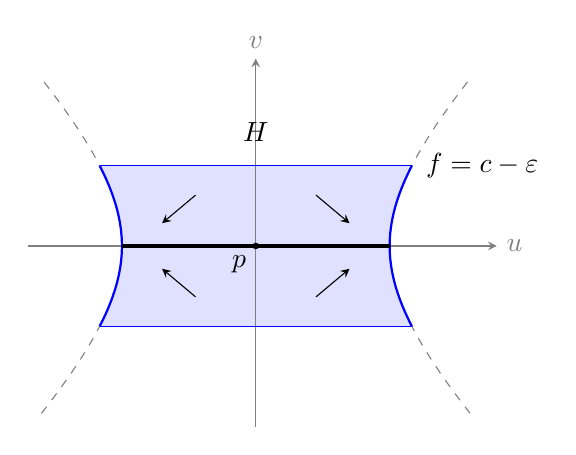
\begin{tikzpicture}[scale=1.7,>=stealth]
	\fill[blue!12] plot[domain=-.6:.6,samples=40] ({sqrt(1+\x*\x)},\x) -- plot[domain=.6:-.6,samples=40] ({-sqrt(1+\x*\x)},\x) -- cycle;
	\draw[->,gray] (-1.7,0)--(1.8,0) node[right] {\(u\)};
	\draw[->,gray] (0,-1.35)--(0,1.4) node[above] {\(v\)};
	\draw[dashed,gray] plot[domain=-1.25:1.25,samples=50] ({sqrt(1+\x*\x)},\x);
	\draw[dashed,gray] plot[domain=-1.25:1.25,samples=50] ({-sqrt(1+\x*\x)},\x);
	\draw[thick,blue] plot[domain=-.6:.6,samples=40] ({sqrt(1+\x*\x)},\x);
	\draw[thick,blue] plot[domain=-.6:.6,samples=40] ({-sqrt(1+\x*\x)},\x);
	\draw[blue] ({-sqrt(1.36)},.6)--({sqrt(1.36)},.6);
	\draw[blue] ({-sqrt(1.36)},-.6)--({sqrt(1.36)},-.6);
	\draw[very thick] (-1,0)--(1,0);
	\draw[->] (.45,.38)--(.7,.17);
	\draw[->] (-.45,.38)--(-.7,.17);
	\draw[->] (.45,-.38)--(.7,-.17);
	\draw[->] (-.45,-.38)--(-.7,-.17);
	\fill (0,0) circle (.025) node[below left] {\(p\)};
	\node at (0,.85) {\(H\)};
	\node[anchor=west] at (1.2,.6) {\(f=c-\varepsilon\)};
\end{tikzpicture}

	\caption[临界点附近的把手]{二维指标一模型 \(f-c=-u^2+v^2\)。阴影块 \(H\) 沿左右两段粗曲线贴到旧次水平集；中心线是核心圆盘。下降向量场沿 \(u\) 方向向外、沿 \(v\) 方向向内，将剩余闭带送入旧区域与新块的并。}
	\label{g2:fig:morse-local-handle}
\end{figure}

局部二次型还提供了控制剩余空间的向量场。在这个坐标域内选 Euclid 度量，则负梯度为
\[
	X=(2u,-2v),\qquad Xf=-4(|u|^2+|v|^2).
\]
在自由面 \(|v|=r\) 上，有 \(X(|v|^2-r^2)=-4r^2<0\)，所以流从外面进入 \(H\)；在旧水平 \(f=c-\varepsilon\) 上，它也严格指向旧次水平集。除原点外，高度一直下降。这两个明确的不等式将局部模型与整体流联系起来。

\subsection{把手附着映射与指标}
\label{g2:subsec:1702:03}
\begin{definition}\label{g2:def:morse-handle}
	设 \(W\) 为光滑 \(n\) 维带边界流形，\(0\le\lambda\le n\)。一个\term[bashou]{指标 \(\lambda\) 的把手}[handle of index \(\lambda\)]是乘积 \(D^\lambda\times D^{n-\lambda}\)，其附着面为 \(S^{\lambda-1}\times D^{n-\lambda}\)。给定光滑嵌入
	\[
		\varphi:S^{\lambda-1}\times D^{n-\lambda}\longrightarrow\partial W,
	\]
	将附着面上的点 \((x,w)\) 与 \(\varphi(x,w)\) 识别，再将接缝的角磨圆，称为向 \(W\) 附着这个把手。\(D^\lambda\times\{0\}\) 称为\term[hexinyuanpan]{核心圆盘}[core disk]，\(\{0\}\times D^{n-\lambda}\) 称为\term[gonghexinyuanpan]{共核心圆盘}[cocore disk]。
\end{definition}

附着数据包含整个有厚度的球面邻域。仅指定中心球面 \(S^{\lambda-1}\times\{0\}\) 的像，还没有说明横向圆盘怎样放置；后续手术中的法标架正来自这份数据。

\begin{theorem}[Morse 把手附着定理]\label{g2:thm:morse-handle-attachment}
	设 \(M\) 为光滑 \(n\) 维流形，\(f:M\to\mathbb R\) 光滑，\(a<b\) 为正则值，且紧闭带 \(f^{-1}([a,b])\) 位于 \(M\) 内部。若其中恰有一个临界点 \(p\)，该点非退化且指标为 \(\lambda\)，则 \(M^b\) 微分同胚于向 \(M^a\) 附着一个指标 \(\lambda\) 的把手并磨圆所得的流形。附着映射可由式\eqref{g2:eq:morse-handle-parametrization}的附着面沿无临界带下降到 \(f^{-1}(a)\) 得到。
\end{theorem}
\begin{proof}
	令 \(c=f(p)\)。先取充分小的 \(\varepsilon>0\)，使 \(a<c-\varepsilon<c+\varepsilon<b\)，并能使用上面的坐标块。两侧闭带 \([a,c-\varepsilon]\)、\([c+\varepsilon,b]\) 都没有临界点，\cref{g2:prop:morse-regular-band}将它们识别为领带。因此只需处理 \(a=c-\varepsilon\)、\(b=c+\varepsilon\)；最后把附着映射沿下方的流搬回原来的水平即可。

	记 \(A=M^{c-\varepsilon}\)，取式\eqref{g2:eq:morse-handle-parametrization}中的 \(H\)，令 \(K=A\cup H\)。式\eqref{g2:eq:morse-handle-attaching-face}说明，\(K\) 确实是沿嵌入 \(\Phi|_{S^{\lambda-1}\times D^\mu}\) 作出的把手附着商：两块的交恰为附着面，且 \(H\) 紧，故这个商到它们在 \(M\) 中的并是同胚。坐标参数化给出了新块的光滑结构。

	将局部 Euclid 度量与外部任意度量用单位分解拼接，使其在 \(H\) 的一个邻域内仍为 Euclid 度量。令 \(X=-\operatorname{grad}f\)。旧边界上 \(Xf<0\)，新块的自由面上 \(X(|v|^2-r^2)<0\)，所以 \(X\) 在 \(K\) 的每个边界面都朝向内部。它的唯一零点 \(p\) 已在 \(K\) 内部。

	先把交界的角变成光滑边界。若 \(0<\lambda<n\)，角附近可用两个独立的横向函数
	\[
		s=f-c+\varepsilon,\qquad t=|v|^2-r^2
	\]
	描述 \(K=\{s\le0\}\cup\{t\le0\}\)。两者的微分在 \(s=t=0\) 处线性无关：此处 \(u,v\) 均非零，而 \(\mathrm{d}t\) 没有 \(u\) 分量。取光滑偶函数 \(\eta_\delta\)，满足 \(\eta_\delta(z)\ge|z|\)、\(|\eta_\delta'(z)|\le1\)，并在 \(|z|\ge\delta\) 时等于 \(|z|\)。例如将绝对值与支集很小的偶非负平滑核卷积即可。把角附近的边界换成
	\[
		m_\delta(s,t)=\frac{s+t-\eta_\delta(s-t)}2=0,
	\]
	并取 \(m_\delta\le0\) 一侧。它包含原来的 \(K\)，且新增边界只发生在 \(|s|,|t|\) 都很小的地方，因此与角邻域外的原边界精确拼接。两偏导非负且之和为一；由于 \(Xs<0\)、\(Xt<0\)，有 \(Xm_\delta<0\)，所以新边界光滑，\(X\) 仍严格朝内。记磨圆后的区域为 \(K_\delta\)。取 \(\delta\) 小，可使 \(K_\delta\setminus A\subset\{f<c+\varepsilon\}\)。指标为 \(0\) 或 \(n\) 时没有这种角，直接令 \(K_\delta=K\)。

	剩下的紧区域 \(M^{c+\varepsilon}\setminus\operatorname{int}_M K_\delta\) 没有临界点。其上 \(|\operatorname{grad}f|^2\) 有严格正的下界。因此从新增边界 \(B=\partial K_\delta\cap f^{-1}([c-\varepsilon,c+\varepsilon])\) 沿 \(-X\) 向外运动，必在有限时间到达 \(f=c+\varepsilon\)：若一直不到达，高度将以一个固定正速度增加而始终不超过该值，矛盾。反向轨道同样在有限时间到达 \(B\)。光滑依赖与隐函数定理说明首次到达时间 \(\tau(z)>0\) 随 \(z\in B\) 光滑变化，因为两端的向量场都横截边界。流遂给出
	\[
		M^{c+\varepsilon}\setminus\operatorname{int}_M K_\delta
		\cong\{(z,t):z\in B,\ 0\le t\le\tau(z)\}.
	\]
	没有外部边界的连通分支已完全包含于 \(K_\delta\)，在此乘积中不出现。

	这段外部乘积可以吸收到 \(K_\delta\) 的一个内部领圈中。具体说，在每条领线的区间 \([-h,\tau(z)]\) 上，选依赖 \(z\) 光滑、在左端附近恒等的严格递增微分同胚到 \([-h,0]\)；\(B\) 紧，故可统一取 \(h>0\)。这样的区间映射可由一个处处为正、左端等于一的光滑密度积分而成，再使总积分等于 \(h\)。与领圈外的恒等映射拼接，得到 \(M^{c+\varepsilon}\cong K_\delta\)。至此既确定了附着面，也处理了剩余空间和接缝光滑结构。
\end{proof}

上面证明还给出一个相对结论，后面计算同调时会用到：未磨圆的 \(K=A\cup H\) 是 \(M^{c+\varepsilon}\) 的强形变收缩像。沿 \(X\) 流到第一次进入 \(K\) 即停下，进入时间在各光滑面附近由横截性连续变化；角附近它是到两个边界面的时间的较小者，仍连续。剩余紧区域中 \(Xf\) 有严格负的上界，保证每条轨道都在有限时间进入。将这段时间乘以同伦参数，就得到固定 \(K\)、从而固定 \(A\) 的收缩。这个结论不需要先磨圆。

\ProseParagraphBreak

在曲面上，指标零把手是一个新圆盘；指标一把手是沿两条短边接上的带；指标二把手沿整个圆周填入一个圆盘。中间那条带可能连接两个原有分支，也可能把同一个分支的两个部位连起来。局部指标决定新增块的形状，附着位置则决定全局拓扑怎样改变。

\subsection{从把手到胞腔同伦类型}
\label{g2:subsec:1702:04}
把手中 \(D^{n-\lambda}\) 的厚度可以连续压掉，但在压缩时必须固定已经贴在旧区域上的整个附着面。直接将 \((x,w)\) 送到 \((x,(1-s)w)\) 会移动附着面，无法与旧区域上的恒等映射拼接。下面给出保持粘合位置的收缩。

\begin{lemma}\label{g2:lem:handle-core-retraction}
	乘积圆盘 \(D^\lambda\times D^\mu\) 强形变收缩到
	\[
		Q=(D^\lambda\times\{0\})\cup(S^{\lambda-1}\times D^\mu).
	\]
	因此沿 \(\varphi\) 附着把手所得的空间强形变收缩到沿 \(\varphi(x,0)\) 附着核心 \(D^\lambda\) 所得的空间，且收缩固定旧空间。
\end{lemma}
\begin{proof}
	给出一条先增大 \(|x|\)、同时减小 \(|w|\)，直到碰到 \(|x|=1\) 或 \(w=0\) 的路径。置
	\[
		T(x,w)=\min\{|w|,-\log|x|\},\qquad
		T(0,w)=|w|.
	\]
	当 \(w\ne0\) 时，令
	\[
		F_s(x,w)=\left(e^{sT(x,w)}x,
		\left(1-\frac{sT(x,w)}{|w|}\right)w\right),
		\qquad 0\le s\le1;
	\]
	当 \(w=0\) 时取 \(F_s(x,0)=(x,0)\)。因为 \(T\le-\log|x|\)、\(T\le|w|\)，路径始终留在乘积圆盘内。\(x\to0\) 时 \(-\log|x|\to\infty\)，所以 \(T=|w|\) 在其附近成立；\(w\to0\) 时 \(T\to0\)，第二分量的范数至多为 \(|w|\)。这些估计保证整个公式连续。\(s=1\) 时至少达到 \(|x|=1\) 或 \(w=0\) 之一；原本就在 \(Q\) 上的点有 \(T=0\)，始终不动。\(\lambda=0\) 时这就是圆盘到中心的径向收缩，\(\mu=0\) 时全部点已在核心上。最后在旧空间上取恒等映射，因附着面逐点不动，公式经附着商下降为所需的强形变收缩。
\end{proof}

由把手附着定理后的相对收缩及此引理，单临界点跨越给出
\begin{equation}\label{g2:eq:morse-cell-attachment}
	M^{c+\varepsilon}\simeq
	M^{c-\varepsilon}\cup_\alpha D^\lambda,
	\qquad
	\alpha(x)=\Phi(x,0),\quad x\in S^{\lambda-1},
\end{equation}
且同伦等价固定旧次水平集。这一步把负二次项的个数变成了实际附着胞腔的维数。

\begin{corollary}\label{g2:cor:morse-cell-type}
	设 \(M\) 为紧光滑 \(n\) 维流形。若 \(M\) 无边界，取任意 Morse 函数 \(f\)；若有边界，设 \(f=b-t\) 于一个向内参数为 \(t\) 的领圈，\(f<b\) 于内部，且全部内部临界点非退化。记指标 \(k\) 的临界点数为 \(m_k\)。则 \(M\) 具有有限把手分解，并同伦等价于一个恰有 \(m_k\) 个 \(k\) 胞腔的有限 CW 复形。
\end{corollary}
\begin{proof}
	非退化临界点孤立；紧性和边界附近无临界点保证它们只有有限多个。由\cref{g2:prop:distinct-morse-critical-values}的小扰动，可分开临界值且保持临界点指标，并在带边界情形保持领圈上的函数。取低于最小临界值的水平，此时次水平集为空。在相邻临界值之间取正则水平，逐次应用\cref{g2:thm:morse-handle-attachment}，便得到所述有限把手分解。带边界时最后只剩一个无临界的边界领带，吸收这段领带不再增加把手。

	逐次使用式\eqref{g2:eq:morse-cell-attachment}，每次只增加一个同指标的胞腔。这里附着次序由临界值排列，未必按指标排列，所以还须说明能得到通常的 CW 结构。假设前一阶段已用有限 CW 复形 \(L\) 表示，把新附着映射先送入 \(L\)，再用\cref{g2:thm:cellular-approximation}将 \(S^{\lambda-1}\to L\) 同伦到 \(L^{\lambda-1}\)。\cref{g2:prop:homotopic-attaching-maps}说明这不改变附着后的同伦型，并保持旧空间。将旧空间换成同伦等价的 \(L\) 时，同样可把同伦逆与两段逆同伦放在附着球面的映射柱上，再用圆盘对的同伦延拓性质延入圆盘；\cref{g2:thm:cofibration-pushout}保证映射柱可压回普通附着，故所得空间仍同伦等价。于是每一步都保留已有胞腔，只向正确的低维骨架增加一个 \(\lambda\) 胞腔。有限归纳得到所需 CW 复形，并保持各维胞腔数。
\end{proof}

这两个滤过承担不同任务：实际次水平集按高度增长，CW 骨架按维数增长。前者保留临界点穿越的几何过程，后者适合使用第3章的胞腔链复形。把二者通过相对同伦等价联系起来，才能将临界点个数与同调维数比较。
% 纲要条目排为编号小节标题，并进入目录与书签；说明段仍保留于纲要注释中。

% !TeX root = ../../Book2.tex
% 纲要标题：### 17.3 Morse 不等式
% 纲要位置：几何学计划纲要.md，第 1673 行。
% 正文状态：未撰写；本文件目前是框架。

% 纲要内容开始
% 
% * 相对同调的临界贡献
% * 滤过链群与弱不等式
% * 强不等式和 Euler 等式
% * 完美 Morse 函数及反例
% 
% 纲要内容结束

\section{Morse 不等式}
\label{g2:sec:1703}

待撰写

\subsection{相对同调的临界贡献}
\label{g2:subsec:1703:01}
待撰写

\subsection{滤过链群与弱不等式}
\label{g2:subsec:1703:02}
待撰写

\subsection{强不等式和 Euler 等式}
\label{g2:subsec:1703:03}
待撰写

\subsection{完美 Morse 函数及反例}
\label{g2:subsec:1703:04}
待撰写
% 纲要条目排为编号小节标题，并进入目录与书签；说明段仍保留于纲要注释中。

% !TeX root = ../../Book2.tex
% 纲要标题：### 17.4 Poincaré–Hopf 的证明
% 纲要位置：几何学计划纲要.md，第 1680 行。
% 正文状态：未撰写；本文件目前是框架。

% 纲要内容开始
% 
% * 梯度零点指标与 Morse 指标
% * 指标和的扰动不变性
% * 任意孤立零点向量场的公式
% * 边界版本及指向条件
% 
% 纲要内容结束

\section{Poincaré–Hopf 的证明}
\label{g2:sec:1704}

待撰写

\subsection{梯度零点指标与 Morse 指标}
\label{g2:subsec:1704:01}
待撰写

\subsection{指标和的扰动不变性}
\label{g2:subsec:1704:02}
待撰写

\subsection{任意孤立零点向量场的公式}
\label{g2:subsec:1704:03}
待撰写

\subsection{边界版本及指向条件}
\label{g2:subsec:1704:04}
待撰写
% 纲要条目排为编号小节标题，并进入目录与书签；说明段仍保留于纲要注释中。

% !TeX root = ../../Book2.tex
% 纲要标题：### 17.5 把手方法的深入应用
% 纲要位置：几何学计划纲要.md，第 1637 行。
% 正文状态：未撰写；本文件目前是框架。

% 纲要内容开始
% 
% * 曲面与射影空间的分解
% * 把手消去的局部条件
% * 配边与手术的接口
% 
% ---
% 
% 纲要内容结束

\section{把手方法的深入应用}
\label{g2:sec:1705}

待撰写

\subsection{曲面与射影空间的分解}
\label{g2:subsec:1705:01}
待撰写

\subsection{把手消去的局部条件}
\label{g2:subsec:1705:02}
待撰写

\subsection{配边与手术的接口}
\label{g2:subsec:1705:03}
待撰写
% 纲要条目排为编号小节标题，并进入目录与书签；说明段仍保留于纲要注释中。


\begin{chaptersummary}
待撰写
\end{chaptersummary}

\BookExercises
待撰写

% !TeX root = ../../Book2.tex
% 纲要标题：## 第18章*　Morse–Smale 同调：轨线、紧化与粘合
% 纲要位置：几何学计划纲要.md，第 1695 行。
% 正文状态：未撰写；本文件目前是框架。

% 纲要内容开始
% 
% > 本章目标与证明范围：闭光滑流形、Morse–Smale 数据、F₂ 系数下完成整个同调构造及与奇异同调比较。整数取向另列进阶节，不以“端点成对出现”代替紧化为流形的证明。
% 
% 纲要内容结束

\OptionalChapter{Morse–Smale 同调：轨线、紧化与粘合}{g2:ch:18}
\BookChapterNumber{g2:ch:18}

\begin{chapterabstract}
待撰写
\end{chapterabstract}

\begin{learninggoals}
待撰写
\end{learninggoals}

待撰写

% !TeX root = ../../Book2.tex
% 纲要标题：### 18.1 梯度流的局部动力学
% 纲要位置：几何学计划纲要.md，第 1699 行。
% 正文状态：初稿；尚未正式审核。

% 纲要内容开始
% 
% * 双曲临界点和稳定流形定理
% * 稳定、不稳定流形的维数
% * Morse–Smale 扰动
% * 轨线空间及平移群商
% 
% 纲要内容结束

\section{梯度流的局部动力学}
\label{g2:sec:1801}

上一章的胞腔边界由把手的附着映射定义。若要用下降轨线直接计算边界，首先必须回答：从一个临界点出发的轨线有多少自由度，能够流向另一个临界点的条件又消去多少自由度？稳定与不稳定流形给出这两组参数；横截性保证相交后的维数等于预期值。最后还要删去沿同一条轨线移动时间原点的一个参数。

\subsection{双曲临界点和稳定流形定理}
\label{g2:subsec:1801:01}

在 Euclid 空间中，线性方程 \(\dot z=Az\) 的解为 \(e^{tA}z(0)\)。特征值实部为负的方向在正时间收缩，实部为正的方向在负时间收缩。若没有实部为零的特征值，两类方向便有严格的指数间隔。

\begin{definition}\label{g2:def:hyperbolic-zero}
	设光滑向量场 \(X\) 在 \(p\) 处为零。若线性化 \(\mathrm D_pX:\mathrm T_pM\to\mathrm T_pM\) 的复特征值都不在虚轴上，就称 \(p\) 为\term[shuangqulingdian]{双曲零点}[hyperbolic zero]。实部为负、为正的广义特征空间分别记为 \(E^s_p,E^u_p\)，称为稳定与不稳定子空间。
\end{definition}

线性化在零点处按共轭变换，与第16章使用的 \(\mathrm D_pX\) 是同一对象。对负梯度 \(X=-\operatorname{grad}_g f\)，在 Morse 临界点处有
\[
	\mathrm D_pX=-G^{-1}H,
\]
其中 \(G\) 为正定度量矩阵，\(H\) 为 Hessian 矩阵。它与对称矩阵 \(-G^{-1/2}HG^{-1/2}\) 相似，所以全部特征值实且非零。若临界点的 Morse 指标为 \(\lambda\)，正特征值有 \(\lambda\) 个，负特征值有 \(n-\lambda\) 个。

\begin{theorem}[局部稳定流形定理]\label{g2:thm:hyperbolic-stable-manifold}
	设 \(X\) 是光滑流形上的光滑向量场，\(p\) 为双曲零点。则在 \(p\) 的邻域内存在光滑嵌入圆盘 \(W^s_{\mathrm{loc}}(p)\)、\(W^u_{\mathrm{loc}}(p)\)，分别切于 \(E^s_p,E^u_p\)。充分靠近 \(p\)、在所有正时间内留在该邻域的轨线，恰从局部稳定流形出发，并指数趋于 \(p\)；负时间的对应结论对局部不稳定流形成立。这里的“局部”允许缩小圆盘及用于控制轨线的邻域。
\end{theorem}
\begin{proof}
	给出稳定流形的构造；将时间反向便得到另一部分。取以 \(p\) 为零的坐标，写
	\[
		X(z)=Az+R(z),\qquad R(0)=0,\qquad \mathrm DR(0)=0.
	\]
	记 \(P_s,P_u\) 为沿不变分解 \(E^s\oplus E^u\) 的投影。由矩阵指数的 Jordan 形式，可选 \(a>0,C\ge1\)，使
	\[
		\lVert e^{tA}P_s\rVert\le Ce^{-at},\qquad
		\lVert e^{-tA}P_u\rVert\le Ce^{-at}\quad(t\ge0).
	\]
	多项式因子可吸收到稍慢的指数中。将 \(R\) 乘以小球上的截断函数，可在整个坐标空间得到全局 Lipschitz 函数，其 Lipschitz 常数 \(L\) 任意小，且在更小球内仍是原来的 \(R\)。这里 \(\mathrm DR(0)=0\) 同时控制 \(R\) 的导数和截断产生的项。

	固定 \(0<\beta<a\)，考虑连续路径的完备赋范空间
	\[
		\mathcal B_\beta=
		\left\{z:[0,\infty)\to E^s\oplus E^u:
		\lVert z\rVert_\beta=\sup_{t\ge0}e^{\beta t}|z(t)|<\infty\right\}.
	\]
	给定稳定初值 \(\xi\in E^s\)，把寻找轨线改写成寻找下式的不动点：
	\begin{equation}\label{g2:eq:stable-integral-equation}
		\begin{aligned}
			(\mathcal T_\xi z)(t)
			={}&e^{tA}\xi+\int_0^t e^{(t-s)A}P_sR(z(s))\,\mathrm ds\\
			&-\int_t^\infty e^{(t-s)A}P_uR(z(s))\,\mathrm ds.
		\end{aligned}
	\end{equation}
	第一项把稳定初值向前推进；最后一项从未来施加“没有增长分量”的条件。这正是决定不稳定初值所需的额外约束。两项积分分别满足
	\[
		\lVert\mathcal T_\xi z-\mathcal T_\xi w\rVert_\beta
		\le CL\left(\frac1{a-\beta}+\frac1{a+\beta}\right)
		\lVert z-w\rVert_\beta.
	\]
	例如第一项积分的加权估计为
	\[
		e^{\beta t}\int_0^t Ce^{-a(t-s)}L e^{-\beta s}\,\mathrm ds
		\le \frac{CL}{a-\beta}.
	\]
	选 \(L\) 使总常数 \(\kappa<1\)，逐次迭代 \(\mathcal T_\xi\) 即得唯一不动点 \(z_\xi\)，并有
	\[
		\lVert z_\xi\rVert_\beta\le\frac{C}{1-\kappa}|\xi|.
	\]
	取 \(\xi\) 足够小，这条路径始终处在原向量场未被截断的球中。对积分式求导可得 \(\dot z_\xi=X(z_\xi)\)，而 \(P_sz_\xi(0)=\xi\)。于是初值集合是图像
	\[
		\xi\longmapsto \xi+h(\xi),\qquad
		h(\xi)=-\int_0^\infty e^{-sA}P_uR(z_\xi(s))\,\mathrm ds.
	\]

	还需说明图像光滑，而不只连续。截断后 \(R\) 的各阶导数有界；在上述加权范数中，对积分逐次求导的估计仍由指数积分控制。\(\mathrm D_z\mathcal T_\xi\) 的算子范数小于 \(\kappa\)，因此
	\[
		(I-\mathrm D_z\mathcal T_\xi)^{-1}
		=\sum_{j=0}^\infty(\mathrm D_z\mathcal T_\xi)^j
	\]
	一致收敛。对不动点等式作差商，再移项乘上这个逆，便得 \(z_\xi\) 对 \(\xi\) 的一阶导数；迭代同一步骤得到所有阶导数及其连续性。故 \(h\) 光滑。由于 \(\mathrm DR(0)=0\)，在零路径处求导得到 \(\mathrm Dh(0)=0\)，图像切于 \(E^s\)。

	最后验证刻画的唯一性。若原方程的一条正向轨线始终留在足够小球内，它是有界路径。变参数公式在不稳定分量上从 \(t\) 积分至 \(T\)，再令 \(T\to\infty\)；因 \(e^{(t-T)A}P_uz(T)\to0\)，得到\eqref{g2:eq:stable-integral-equation}。同一算子在普通有界连续路径范数（即 \(\beta=0\)）中也为收缩，可预先将 \(L\) 取得同时满足这一要求。因此该有界路径必等于已构造的 \(z_\xi\)，从而指数衰减并从图像出发。流的唯一性保证图像在轨线仍处于局部邻域期间不变。这完成了稳定流形的构造与刻画。
\end{proof}

非线性稳定流形一般不是线性子空间。例如 \(\dot u=u+v^2,\ \dot v=-v\) 的稳定流形为 \(u=-v^2/3\)，它在零处切于 \(v\) 轴；后面的习题将直接解出这一图像。线性化确定切方向，积分方程则决定曲面本身怎样弯曲。

\subsection{稳定、不稳定流形的维数}
\label{g2:subsec:1801:02}

本章在闭流形上进行计数。紧性保证光滑向量场的流 \(\Phi_t\) 对所有 \(t\in\mathbb R\) 存在，这里使用第一卷第13章第2节的紧流形完备性。对零点 \(p\)，定义
\[
	W^s(p)=\{x:\lim_{t\to+\infty}\Phi_t(x)=p\},\qquad
	W^u(p)=\{x:\lim_{t\to-\infty}\Phi_t(x)=p\}.
\]
它们分别称为\term[wendingliuxing]{稳定流形}[stable manifold]与\term[buwendingliuxing]{不稳定流形}[unstable manifold]。\symidx{\(W^s(p),W^u(p)\)：稳定与不稳定流形}

\begin{proposition}\label{g2:prop:morse-stable-unstable}
	设 \(M^n\) 为闭光滑流形，\(f:M\to\mathbb R\) 为 Morse 函数，\(X=-\operatorname{grad}_g f\)。对指标为 \(\lambda(p)\) 的临界点 \(p\)，\(W^s(p)\)、\(W^u(p)\) 具有自然的单射浸入流形结构，维数分别为 \(n-\lambda(p)\)、\(\lambda(p)\)。在 \(p\) 处，它们的切空间分别是 \(\mathrm D_pX\) 的稳定与不稳定子空间。
\end{proposition}
\begin{proof}
	上一小节已经证明 \(p\) 双曲，并计算了两种线性子空间的维数。局部稳定图像与其各个向后流像
	\[
		\Phi_{-t}(W^s_{\mathrm{loc}}(p)),\qquad t\ge0,
	\]
	覆盖 \(W^s(p)\)：趋于 \(p\) 的轨线在充分大时间后留在局部邻域。局部图像上的稳定坐标满足 \(\dot\xi=A_s\xi+O(|\xi|^2)\)。正定二次型
	\[
		Q(\xi)=\int_0^\infty |e^{tA_s}\xi|^2\,\mathrm dt
	\]
	沿该方程的导数为 \(-|\xi|^2+O(|\xi|^3)\)，所以足够小的 \(Q\) 子水平椭球给出正向不变的局部圆盘。因而可只取整数时间 \(t=0,1,2,\ldots\)，得到递增的圆盘族。相邻圆盘的重叠转换由光滑流给出，其微分可逆；因此这些图拼成同维光滑流形，包含到 \(M\) 的映射为单射浸入。对反向流作相同构造得到 \(W^u(p)\)。切空间与维数来自局部稳定流形定理。
\end{proof}

为使断裂点附近的粘合能够写成具体方程，以下选择在 Morse 坐标中具有精确线性表达的下降场。先在\cref{g2:thm:morse-approximation}给出的 Morse 函数上，用\cref{g2:prop:distinct-morse-critical-values}分开临界值。

\begin{definition}\label{g2:def:normalized-morse-data}
	设 \(M\) 为闭光滑流形，\(f\) 为临界值互异的 Morse 函数。若光滑向量场 \(X\) 满足 \(Xf<0\) 于非临界点，并且在每个临界点的某张 Morse 坐标中有
	\begin{equation}\label{g2:eq:normalized-negative-gradient}
		f=f(p)-|u|^2+|v|^2,\qquad
		X(u,v)=(2u,-2v),
		\quad u\in\mathbb R^{\lambda(p)},\ v\in\mathbb R^{n-\lambda(p)},
	\end{equation}
	就把 \((f,X)\) 称为本章的正规化 Morse 数据。
\end{definition}

这种数据总能选到。取各临界点互不相交的 Morse 坐标邻域，在其中规定 Euclid 度量，再用单位分解与外部度量拼接，保持更小邻域内的度量不变。所得 \(X=-\operatorname{grad}_g f\) 满足\eqref{g2:eq:normalized-negative-gradient}。反过来，定义中的每个 \(X\) 也确实是某个光滑度量的负梯度：在非临界区域令 \(\alpha=-\mathrm df\)，则 \(\alpha(X)>0\)，并有分解
\[
	\mathrm TM=\mathbb RX\oplus\ker\alpha.
\]
在 \(\ker\alpha\) 上任选正定内积 \(h\)，规定
\[
	g(aX+v,bX+w)=ab\,\alpha(X)+h(v,w).
\]
于是 \(g(X,\cdot)=\alpha=-\mathrm df\)。临界点附近的 Euclid 度量满足同一等式，用单位分解拼接时此线性等式仍保持，得到所需全局光滑度量。

\ProseParagraphBreak

对正规化数据，局部稳定与不稳定圆盘分别为 \(u=0\)、\(v=0\)，轨线的表达为
\[
	u(t)=e^{2t}u(0),\qquad v(t)=e^{-2t}v(0).
\]
这项选择将高阶项放到临界点以外，后面可直接用停留时间 \(T\) 与参数 \(e^{-2T}\) 描述经过临界邻域的长轨线。第18.4节将通过延拓映射比较不同的数据选择。

\ProseParagraphBreak

此时全局稳定流形还可明确参数化为 \(\mathbb R^{n-\lambda(p)}\)。取局部稳定球面 \(|v|=\varepsilon\)，对 \(v\ne0\) 定义
\[
	\iota_s(v)=\Phi_{-\frac12\log(|v|/\varepsilon)}
	\left(0,\varepsilon\frac{v}{|v|}\right),\qquad \iota_s(0)=p.
\]
当 \(|v|\le\varepsilon\) 时，这就是局部坐标点 \((0,v)\)；当 \(|v|>\varepsilon\) 时，则沿完整流向后延拓。每条非恒定稳定轨线恰好经过局部球面一次，故它给出全局一一参数化，逆映射由光滑的到达时间给出。零维情形直接为一个点。反向时间同样参数化 \(W^u(p)\cong\mathbb R^{\lambda(p)}\)。这里采用的是前述自然浸入流形结构；特别地，这两个流形都可缩，后面可以在它们上面连续选择方向。

\subsection{Morse–Smale 扰动}
\label{g2:subsec:1801:03}

从 \(p\) 出发并流向 \(q\) 的非恒定轨线，其每个点都在 \(W^u(p)\cap W^s(q)\) 中。两个流形若相切，交集可能有多余维数，计数也会对扰动不稳定。因此需要第14章的横截条件。

\begin{definition}\label{g2:def:morse-smale-data}
	闭光滑流形上的正规化 Morse 数据 \((f,X)\) 满足下列横截性时，称它满足\term[Morse-Smale tiaojian]{Morse--Smale 条件}[Morse--Smale condition]：
	\[
		W^u(p)\pitchfork W^s(q)\qquad
		\text{对全部临界点 }p,q,
	\]
	条件在相交点处的含义是两切空间之和为整个 \(\mathrm T_xM\)；对浸入流形用其上述自然流形结构判断。
\end{definition}

\begin{theorem}[Morse--Smale 扰动]\label{g2:thm:morse-smale-existence}
	设 \((f,X_0)\) 是闭光滑流形上的正规化 Morse 数据，并在各临界点选定更小的、两两不交的闭坐标邻域。则 \(X_0\) 的每个 \(C^\infty\) 邻域中都有光滑向量场 \(X\)，使 \((f,X)\) 满足 Morse--Smale 条件，且 \(X=X_0\) 于这些闭邻域的某个固定邻域。函数 \(f\) 及全部临界点均保持不变。
\end{theorem}
\begin{proof}
	把问题化为有限时间的流映射横截性，这样每次扰动只需有限个参数。对每个临界点 \(p\)，在固定线性邻域内部取局部出球面
	\[
		S_p^-=\{(u,0):|u|=\varepsilon_p\},
	\]
	维数为 \(\lambda(p)-1\)；对每个 \(q\) 取入球面
	\[
		S_q^+=\{(0,v):|v|=\varepsilon_q\},
	\]
	维数为 \(n-\lambda(q)-1\)。空维球面取空集。任何从 \(p\) 到 \(q\) 的非恒定轨线，都恰好经过这两个球面一次。考察
	\[
		E_X:S_p^-\times(0,\infty)\longrightarrow M,\qquad
		E_X(a,T)=\Phi_T^X(a).
	\]
	条件 \(E_X\pitchfork S_q^+\) 等价于 \(W^u(p)\pitchfork W^s(q)\)：\(E_X\) 的微分包含不稳定方向及流方向，而在入球面上
	\(\mathrm T W^s(q)=\mathrm T S_q^+\oplus\mathbb RX\)。
	同一流方向已经在 \(E_X\) 的像内，故两种切空间满秩条件相同。\(p=q\) 的情形在临界点由正、负子空间互补自动成立，且严格下降排除了非恒定同宿轨线。

	先只要求在紧集 \(K_N=S_p^-\times[1/N,N]\) 上横截，\(N\) 为正整数。若 \(E_{X_0}(a,T)\in S_q^+\)，该连接段在两临界邻域之间必经过一个允许扰动的小流盒。对支于该流盒的场 \(Y\)，终点关于 \(X_\theta=X_0+\theta Y\) 的一阶变化为
	\begin{equation}\label{g2:eq:flow-endpoint-variation}
		\left.\frac{\partial}{\partial\theta}\right|_0
		\Phi_T^{X_\theta}(a)
		=\int_0^T
		\mathrm d\Phi_{T-s}^{X_0}\bigl(Y(\Phi_s^{X_0}(a))\bigr)\,\mathrm ds.
	\end{equation}
	这由第一卷第13章第1节的参数光滑依赖及其变分方程得到：对流方程求参数导数，再用基本解矩阵积分。选一小段时间上的光滑截断函数，其积分为一；对任意目标向量 \(w\in\mathrm T_{\Phi_T(a)}M\)，沿这段轨线规定
	\[
		Y(\Phi_s(a))=\rho(s)\,
		(\mathrm d\Phi_{T-s})^{-1}w.
	\]
	用流盒坐标横向延拓并加截断，便得到允许的光滑场，使\eqref{g2:eq:flow-endpoint-variation}恰等于 \(w\)。因 \(f\) 严格下降，流盒可选在一个小高度带中，该轨线不会再次经过其支集。因此有限个这样的场就能在此约束点补足全部终点方向。

	约束点集 \(K_N\cap E_{X_0}^{-1}(S_q^+)\) 紧。取有限覆盖，收集上述有限个场 \(Y_1,\ldots,Y_L\)，得到
	\[
		(a,T,\theta)\longmapsto
		\Phi_T^{X_0+\sum_i\theta_iY_i}(a).
	\]
	在足够小的参数球内，它在 \(K_N\) 附近与 \(S_q^+\) 横截。原来避开 \(S_q^+\) 的其余紧部分仍避开它，因 \(S_q^+\) 闭。由\cref{g2:thm:parametric-transversality}，任意小参数中都有使切片在 \(K_N\) 上横截的选择。充分小的场扰动还保持 \(Xf<0\)：固定临界邻域之外是紧集，原来的 \(-X_0f\) 在那里有正下界。临界邻域内的场完全未改。

	现在同时实现全部条件。临界点对只有有限多个，而 \(N=1,2,\ldots\)，故可把这些紧集横截要求排成可数序列。每项要求由刚才的构造在允许场空间中稠密；由有限时间流的一阶连续依赖及\cref{g2:prop:transversality-open-on-compact}，它又是开条件。逐项选光滑场 \(X_j\)，使第 \(j\) 项及先前各项成立，并把第 \(j\) 次改动的 \(C^j\) 范数取得小于 \(2^{-j}\) 倍的指定容差。每次再为已满足的有限个条件选择保持它们的开邻域，分配后续改动的总误差小于这些邻域的容差。还把所有改动的总 \(C^0\) 误差限制在保持下降条件的界内，并满足最初给定的 \(C^\infty\) 邻域中的有限阶控制。

	于是 \(X_j\) 在每个 \(C^r\) 范数中收敛；在有限坐标覆盖上逐阶取极限，得到光滑 \(X\)。全部紧集横截条件由各自预留的余量保持，固定邻域内的表达也未变。任意有限时间的连接轨线属于某个 \(K_N\)，所以所有不稳定与稳定流形都横截。这便得到所需的 \(X\)。
\end{proof}

这里的扰动改变临界点之间的轨线走向，同时完整保留临界点附近的线性模型。这两种控制将在后面同时使用：横截性给粘合方程的可逆线性部分，局部线性模型给小参数的精确表达。

\subsection{轨线空间及平移群商}
\label{g2:subsec:1801:04}

对不同临界点 \(p,q\)，设 \(\widetilde{\mathcal M}(p,q)\) 为满足
\[
	\dot\gamma(t)=X(\gamma(t)),\qquad
	\lim_{t\to-\infty}\gamma(t)=p,\qquad
	\lim_{t\to+\infty}\gamma(t)=q
\]
的非恒定参数化轨线。由流的唯一性，取值 \(\gamma\mapsto\gamma(0)\) 将其识别为 \(W^u(p)\cap W^s(q)\)。时间平移
\[
	(\tau\cdot\gamma)(t)=\gamma(t+\tau)
\]
只改变零时刻，不改变下降路径。将这一冗余除去，得到\term[guixianmolikongjian]{轨线模空间}[moduli space of trajectories]
\[
	\mathcal M(p,q)=\widetilde{\mathcal M}(p,q)/\mathbb R.
\]
本章的计数都在这个商空间中进行。\symidx{\(\mathcal M(p,q)\)：无参数下降轨线空间}

\begin{proposition}\label{g2:prop:trajectory-quotient}
	设 \((f,X)\) 是闭光滑 \(n\) 维流形上的正规化 Morse--Smale 数据，\(p\ne q\) 为临界点。若 \(\mathcal M(p,q)\ne\varnothing\)，则 \(f(p)>f(q)\)、\(\lambda(p)>\lambda(q)\)，而 \(\mathcal M(p,q)\) 是维数
	\[
		\dim\mathcal M(p,q)=\lambda(p)-\lambda(q)-1
	\]
	的光滑流形。任取 \(f(q)<a<f(p)\) 中的正则值，取唯一交点给出微分同胚
	\begin{equation}\label{g2:eq:trajectory-level-section}
		\mathcal M(p,q)\cong
		W^u(p)\cap W^s(q)\cap f^{-1}(a).
	\end{equation}
	时间平移作用自由且固有。
\end{proposition}
\begin{proof}
	非恒定轨线上 \(\frac{\mathrm d}{\mathrm dt}f(\gamma(t))=Xf<0\)，所以两端临界值严格下降。\cref{g2:thm:transverse-preimage}的交集维数公式给出
	\[
		\dim\widetilde{\mathcal M}(p,q)
		=\lambda(p)+(n-\lambda(q))-n
		=\lambda(p)-\lambda(q).
	\]
	非零流向量 \(X\) 同时切于这两张流形，故交集的非空维数至少为一，得到指标严格下降。沿交集，\(\mathrm df(X)<0\)，所以 \(f=a\) 再切去一维。

	轨线上 \(f\) 连续且严格递减，两端值分别为 \(f(p),f(q)\)，故每条轨线恰有一个点在水平 \(a\) 上。记这个截面为 \(S\)。由到达方程 \(f(\Phi_t(x))=a\) 及其时间导数 \(Xf\ne0\)，隐函数定理给出到达时间对 \(x\) 的光滑依赖。因此
	\[
		S\times\mathbb R\longrightarrow\widetilde{\mathcal M}(p,q),
		\qquad(z,t)\longmapsto\Phi_t(z)
	\]
	为微分同胚；逆映射把一个点送回其唯一截面点，并记录所用时间。于是平移作用对应第二因子上的普通平移，既自由又固有：若初、末两点在两个指定紧集中，它们的时间坐标之差有界，截面坐标也在紧集中，作用映射的相应原像为紧集。取商就得到 \(S\) 的光滑结构及\eqref{g2:eq:trajectory-level-section}。换另一正则水平时，过渡映射是流的首次到达映射，仍光滑，故这个结构不依赖所选水平。
\end{proof}

对于不同临界点，模空间非空的必要条件是指标至少下降一。指标相差一时，商空间为零维；相差二时，它为一维。零维目前只说明每条轨线在附近孤立，是否总共有有限条还要使用下一节的断裂紧性。

\begin{example}\label{g2:exm:sphere-meridian-moduli}
	标准 \(S^n\) 的高度函数只有最高点 \(p\) 与最低点 \(q\)。其负梯度轨线是由北向南的子午线；除去时间平移后，每条子午线由赤道上的唯一交点确定。因此
	\[
		\mathcal M(p,q)\cong S^{n-1}.
	\]
	对 \(n=1\)，它是两条半圆轨线组成的两点集；对 \(n=2\)，它是一圈轨线。将度量在极点附近改成正规化度量，并保持径向方向，可保留这组无参数轨线。这个例子也显示，若不除去平移，即使只有一条几何路径，仍会出现一整条 \(\mathbb R\) 的参数。
\end{example}

% !TeX root = ../../Book2.tex
% 纲要标题：### 18.2 轨线序列和断裂紧化
% 纲要位置：几何学计划纲要.md，第 1706 行。
% 正文状态：初稿；尚未正式审核。

% 纲要内容开始
% 
% * 能量恒等式与临界值下降
% * 选定时间平移后的局部收敛
% * 有限次断裂和能量控制
% * 零维紧性及计数有限性
% 
% 纲要内容结束

\section{轨线序列和断裂紧化}
\label{g2:sec:1802}

轨线可以越来越靠近一个中间临界点，在那里停留越来越久，再继续下降。每一条轨线都从 \(p\) 到 \(q\)，极限却可能要由“从 \(p\) 到 \(r\)”和“从 \(r\) 到 \(q\)”两条轨线合起来描述。要把轨线数用作链复形的系数，首先必须知道这种退化能发生多少次，以及是否还有别的轨线逃失方式。本节利用下降的函数值为轨线选定截点，把紧性问题化成有限个紧水平集中的收敛问题。

\subsection{能量恒等式与临界值下降}
\label{g2:subsec:1802:01}

固定闭光滑流形 \(M\)、Morse 函数 \(f\) 和光滑 Riemann 度量 \(g\)，令 \(X=-\operatorname{grad}_g f\)。前节所选的正规化数据满足这些条件。闭性保证 \(X\) 的流对所有实时间存在：第一卷第13章第2节的紧支完备性定理适用，因为此时整个流形就是一个紧支集。

\begin{proposition}\label{g2:prop:morse-energy-limits}
	设 \(M\) 为闭光滑流形，\(f:M\to\mathbb R\) 为 Morse 函数，\(g\) 为光滑 Riemann 度量。任何非恒定解
	\[
		\dot\gamma(t)=-\operatorname{grad}_g f(\gamma(t)),\qquad t\in\mathbb R,
	\]
	都存在临界点 \(p,q\)，使 \(\gamma(t)\to p\) 当 \(t\to-\infty\)，\(\gamma(t)\to q\) 当 \(t\to+\infty\)。而且 \(f(p)>f(q)\)，并有
	\begin{equation}\label{g2:eq:morse-energy-identity}
		E(\gamma)\coloneqq\int_{-\infty}^{+\infty}|\dot\gamma(t)|_g^2\,\mathrm{d}t
		=f(p)-f(q).
	\end{equation}
\end{proposition}
\begin{proof}
	梯度的定义给出
	\[
		\frac{\mathrm{d}}{\mathrm{d}t}f(\gamma(t))
		=\mathrm{d}f_{\gamma(t)}(\dot\gamma(t))
		=-|\operatorname{grad}_g f(\gamma(t))|_g^2.
	\]
	积分于有限区间 \([a,b]\)，得到
	\[
		\int_a^b|\dot\gamma|_g^2\,\mathrm{d}t
		=f(\gamma(a))-f(\gamma(b)).
	\]
	\(f\) 在紧流形上有界，因此两端的函数值极限存在，且正、负半轴上的能量均有限。还要证明轨线本身收敛，而不只证明其函数值收敛。

	考察正向极限集
	\[
		\omega(\gamma)=\bigcap_{T\ge0}\overline{\{\gamma(t):t\ge T\}}.
	\]
	其中每个集合都是非空紧连通集，且随 \(T\) 增大而递减；因此交也是非空紧连通集。若 \(x\in\omega(\gamma)\) 不是临界点，就可取 \(x\) 的邻域 \(V\)，以及稍大的邻域 \(U\)，使 \(|\operatorname{grad}f|\ge\delta>0\) 于 \(U\)。流的连续性和 \(\overline V\subset U\) 的紧性给出统一的 \(h>0\)：从 \(V\) 出发的轨线在时间 \([0,h]\) 内留在 \(U\)。轨线无限次进入 \(V\)；选取间隔大于 \(h\) 的进入时刻，每次在随后长度 \(h\) 的区间耗费至少 \(h\delta^2\) 的能量，与正向能量有限矛盾。故 \(\omega(\gamma)\) 全由临界点组成。

	Morse 临界点孤立，在紧流形上只有有限个。有限集的非空连通子集只有一个点，因此 \(\omega(\gamma)=\{q\}\)。若轨线不趋于 \(q\)，可取一个离 \(q\) 有正距离的点列，并由紧性取得另一个正向聚点，矛盾。负向极限同理为某个临界点 \(p\)。令有限区间的两端趋于无穷，即得能量恒等式。非恒定轨线在任何有限时刻均不经过临界点，否则由常微分方程解的唯一性，它将恒定；故其能量严格为正，\(f(p)>f(q)\)。
\end{proof}

能量在本章就是下降掉的函数值。它控制的是整个过程的总变化量，并不控制需要多长时间：在临界点附近，梯度很小，轨线可以用很长时间下降很少的高度。这正是断裂极限的来源。

\begin{example}
	在局部标准模型 \(f=c-u^2+v^2\) 中，下降方程为 \(\dot u=2u\)、\(\dot v=-2v\)，所以
	\[
		u(t)=e^{2t}u(0),\qquad v(t)=e^{-2t}v(0).
	\]
	从 \(v=\varepsilon\) 的截面进入，且 \(u(0)=\eta>0\)，到达 \(u=\varepsilon\) 所需的时间为
	\[
		T=\frac12\log\frac{\varepsilon}{\eta}.
	\]
	当 \(\eta\to0\) 时，\(T\to\infty\)；前半段趋于沿 \(v\) 轴进入原点的轨线，后半段经重新选定时间零点后趋于沿 \(u\) 轴离开原点的轨线。原点是两个极限段的共同端点。
\end{example}

\subsection{选定时间平移后的局部收敛}
\label{g2:subsec:1802:02}

非参数轨线没有指定的时间零点。若任意选择参数，同一条轨线作越来越大的平移，便可能在每个有限时间区间都趋于一个恒定临界点。为保留一段真正的运动，应先让轨线在一个固定正则水平上经过时间零点。

\begin{lemma}\label{g2:lem:anchored-trajectory-convergence}
	设 \(M\) 闭，\(X=-\operatorname{grad}_g f\)，其中 \(f\) 为 Morse 函数。设 \(a\) 为正则值，\(\gamma_\nu\) 为满足 \(f(\gamma_\nu(0))=a\) 的下降轨线。则可取子列及一条非恒定下降轨线 \(\gamma\)，使
	\[
		\gamma_\nu\longrightarrow\gamma
		\quad\text{于每个有界时间区间，按 }C^\infty\text{ 收敛}.
	\]
	若所有 \(\gamma_\nu\) 都连接同一对临界点 \(p,q\)，则极限轨线的两个端点 \(p',q'\) 满足
	\[
		f(p)\ge f(p')>a>f(q')\ge f(q).
	\]
\end{lemma}
\begin{proof}
	水平集 \(f^{-1}(a)\) 紧，故可使 \(x_\nu=\gamma_\nu(0)\to x\in f^{-1}(a)\)。设 \(\Phi_t\) 为 \(X\) 的流，则 \(\gamma_\nu(t)=\Phi_t(x_\nu)\)。第一卷第13章第1节的光滑依赖定理说明 \((t,x)\mapsto\Phi_t(x)\) 光滑。限制到任意紧时间区间后，所有阶导数都连续，因而 \(\Phi_t(x_\nu)\to\Phi_t(x)\) 按 \(C^\infty\) 收敛。\(a\) 为正则值，故 \(X(x)\ne0\)，极限轨线非恒定。

	若原轨线连接 \(p,q\)，对每个固定 \(t\) 都有 \(f(q)\le f(\gamma_\nu(t))\le f(p)\)。取极限，再让 \(t\to\pm\infty\)，并用\cref{g2:prop:morse-energy-limits}，便得到所述端点不等式。
\end{proof}

这项引理保留了穿过指定水平的那一段轨线。它的端点可能已经改变，例如原来的 \(p\to q\) 轨线在极限中变成了 \(p'\to q'\)。其余下降过程要到别的水平上重新选定时间零点才能看见。

\ProseParagraphBreak

下面记录一个连接相邻截点的判断。取正则值 \(a>b\)，设 \(\gamma_\nu(0)=x_\nu\in f^{-1}(a)\)，并记其经过 \(f^{-1}(b)\) 的时间为 \(\tau_\nu>0\)，对应点为 \(y_\nu\)。若 \(x_\nu\to x\)、\(y_\nu\to y\)，则：

\begin{itemize}
	\item 若 \(\tau_\nu\) 有界，取子列使其趋于 \(\tau\)，便有 \(y=\Phi_\tau(x)\)，两截点属于同一条极限轨线。
	\item 若 \(\tau_\nu\to\infty\)，则从 \(x\) 出发的正向轨线始终留在 \(f\ge b\)，而从 \(y\) 出发的负向轨线始终留在 \(f\le a\)。若 \([b,a]\) 内恰有一个临界点 \(r\)，两条轨线相应的极限端点就都只能是 \(r\)。
\end{itemize}

第二点的“始终”可逐个固定时间检验：对任意 \(T>0\)，当 \(\tau_\nu>T\) 时，\(f(\Phi_T(x_\nu))\ge b\)，取极限即可；负向论证相同。随后由上一命题，两端必须收敛到带中的临界点。正则端水平不含临界点，带中又只有 \(r\)，因此两段确实在同一个 \(r\) 接合。

\subsection{有限次断裂和能量控制}
\label{g2:subsec:1802:03}

设 \(p\ne q\) 为临界点，且 \(f(p)>f(q)\)。一个从 \(p\) 到 \(q\) 的\term[duanlie guixian]{断裂轨线}[broken trajectory]是有限序列
\[
	\boldsymbol\gamma=(\gamma_1,\ldots,\gamma_\ell),\qquad
	\gamma_i\in\mathcal M(p_{i-1},p_i),\qquad
	p_0=p,\quad p_\ell=q,
\]
其中各段均为非恒定非参数轨线。它的临界值严格下降：
\[
	f(p_0)>f(p_1)>\cdots>f(p_\ell).
\]
两条相接轨线各自拥有时间平移的自由，故断裂轨线记录的是各段的非参数类，没有额外的共同时间参数。未断裂轨线对应 \(\ell=1\)。

\begin{theorem}[断裂轨线紧性]\label{g2:thm:broken-trajectory-compactness}
	设 \(M\) 为闭光滑流形，\(f\) 为临界值互异的 Morse 函数，\(X=-\operatorname{grad}_g f\)。设 \(p,q\) 为满足 \(f(p)>f(q)\) 的临界点。从 \(p\) 到 \(q\) 的下降轨线序列都存在一个有限断裂极限：可取子列、临界点链 \(p=p_0,\ldots,p_\ell=q\) 及时间平移 \(s_{\nu,i}\)，使
	\[
		\gamma_\nu(\,\cdot+s_{\nu,i})\longrightarrow\gamma_i
		\quad\text{于紧时间区间按 }C^\infty\text{ 收敛},
		\qquad
		\gamma_i\in\mathcal M(p_{i-1},p_i).
	\]
	相邻两段的平移满足 \(s_{\nu,i+1}-s_{\nu,i}\to+\infty\)，而能量完整分解为
	\begin{equation}\label{g2:eq:broken-energy-sum}
		E(\gamma_\nu)=f(p)-f(q)=\sum_{i=1}^{\ell}E(\gamma_i).
	\end{equation}
	全部断裂轨线组成一个紧 Hausdorff 空间；其拓扑可由下述有限组正则水平上的交点确定。
\end{theorem}
\begin{proof}
	列出 \(f(q)\) 与 \(f(p)\) 之间的全部临界值，包括端点：
	\[
		c_0=f(p)>c_1>\cdots>c_m=f(q).
	\]
	每个区间 \((c_{j+1},c_j)\) 选一个正则值 \(a_j\)，令 \(L_j=f^{-1}(a_j)\)。每条 \(p\to q\) 轨线恰好与每个 \(L_j\) 相交一次，记交点为 \(x_{\nu,j}\)。有限乘积 \(\prod_{j=0}^{m-1}L_j\) 紧；取共同子列，使所有 \(x_{\nu,j}\to x_j\)。再对有限个相邻水平间的通过时间取子列，使每个时间或者趋于有限值，或者趋于正无穷。

	在 \(x_{\nu,j}\) 处把时间平移为零，由\cref{g2:lem:anchored-trajectory-convergence}得到穿过 \(x_j\) 的完整极限轨线。如果两个相邻水平间的通过时间有限，上面关于相邻截点的判断说明，这两条极限轨线只是同一轨线的不同参数选择，应合并为一段。如果通过时间趋于无穷，两水平之间恰有临界值 \(c_{j+1}\)，且因临界值互异只有一个临界点；同一判断说明，上段的正端点与下段的负端点就是这个点。最上段的负端点只能为 \(p\)：它的函数值介于 \(a_0\) 与 \(f(p)\) 之间，而这一区域仅有临界点 \(p\)。最下段同理以 \(q\) 结束。于是全部非重复段接成所需的临界点链，而不只是互不相关的局部极限。

	为每一段选它穿过的一个 \(L_j\)，以原轨线到达该水平的时刻为 \(s_{\nu,i}\)。跨过相邻两段接点时，通过时间已经趋于无穷，故相邻平移之差也趋于无穷。段数至多为 \(m\)。若将全部不同临界值之间的最小正差记为 \(\Delta\)，还可写出
	\[
		\ell\Delta\le f(p)-f(q).
	\]
	每段的能量由其两端临界值之差给出，有限求和逐项抵消，便得到\eqref{g2:eq:broken-energy-sum}。这条等式说明未被任何局部极限段捕获的能量为零；长时间停留本身没有另带一份正能量。

	最后给出整个断裂空间的拓扑并核实其紧性。任一断裂链都在每个 \(L_j\) 上恰有一个交点，故有评价映射
	\[
		\operatorname{ev}:\overline{\mathcal M}(p,q)
		\longrightarrow\prod_{j=0}^{m-1}L_j.
	\]
	这里 \(\overline{\mathcal M}(p,q)\) 暂表示所有有限断裂链的集合。该映射为单射：一条非恒定轨线由其任意一个点唯一决定，而每段连接两个不同临界值，必穿过所选水平中的至少一个；因而全部截点确定各段及它们的连接次序。用这个单射赋予断裂空间子空间拓扑。

	其像是闭集。事实上，给定一列断裂链及其截点的极限，可能出现的临界点链只有有限种；取子列使链的临界点序列固定。分别对每个非恒定段应用刚才的有限水平论证，使它进一步分裂成有限条轨线，再按原有共同端点串接。得到的仍是从 \(p\) 到 \(q\) 的有限断裂链，且其截点恰为给定极限。因此评价像序列闭。有限乘积是紧度量空间，序列闭即闭，所以断裂空间紧且 Hausdorff。

	在未断裂部分，这个拓扑与正则水平截面的通常拓扑一致：任取一处截点，附近的非断裂轨线到其他固定正则水平的到达时间，由流的光滑依赖和横截性随该截点连续变化；反过来乘积收敛当然蕴含该截点收敛。更换所选正则水平也不改变拓扑，因为同一相邻临界值间没有临界点，流给出两个水平的光滑对应。
\end{proof}

若数据还满足 Morse--Smale 条件，每个非恒定段都满足
\[
	\lambda(p_{i-1})-\lambda(p_i)\ge1,
\]
因为\cref{g2:prop:trajectory-quotient}给出的轨线空间维数为两端指标差减一，非空光滑流形不能有负维数。因此
\[
	\ell\le\lambda(p)-\lambda(q).
\]
能量的临界值下降给出有限性，横截性还把可出现的段数限制在指标差以内。这两种控制分别来自函数的下降和稳定、不稳定流形的相交。

\ProseParagraphBreak

\(\overline{\mathcal M}(p,q)\) 的记号记录了允许断裂后的紧空间。下一节将证明，指标差为二时，每个断裂点都有一条由真实未断轨线形成的半开邻域。因此在链复形所需的零维、一维情形，这个空间确实是原轨线空间的紧化，并具有确定的边界结构。

\begin{lemma}\label{g2:lem:broken-local-crossing}
	设 \((f,g)\) 为闭流形上的正规化 Morse--Smale 数据，未断轨线 \(\gamma_\nu\in\mathcal M(p,q)\) 在上述拓扑中趋于一断裂链 \((\alpha,\beta)\in\mathcal M(p,r)\times\mathcal M(r,q)\)。在 \(r\) 的正规化坐标中选充分小的闭箱
	\[
		B_\varepsilon=\{(u,v):|u|\le\varepsilon,\ |v|\le\varepsilon\},
	\]
	使 \(\alpha\) 沿稳定轴在 \((0,v_0)\) 进入 \(|v|=\varepsilon\)，\(\beta\) 沿不稳定轴在 \((u_0,0)\) 离开 \(|u|=\varepsilon\)。则对充分大的 \(\nu\)，\(\gamma_\nu\) 的相应进入点、离开点趋于 \((0,v_0)\)、\((u_0,0)\)，且这次通过箱子的时间 \(T_\nu\to+\infty\)。
\end{lemma}
\begin{proof}
	在 \(\alpha\) 所穿过的一个正则水平上固定时间零点。评价拓扑的收敛和\cref{g2:lem:anchored-trajectory-convergence}使原轨线在这个锚点附近的任意固定有限时间区间上趋于 \(\alpha\)。从锚点到 \((0,v_0)\) 的时间有限；到达截面处有
	\[
		X(|v|^2-\varepsilon^2)=-4\varepsilon^2\ne0.
	\]
	因此隐函数定理和流的光滑依赖使附近轨线的截面交点连续变化，得到进入点收敛。沿 \(\beta\) 从另一个水平截点向后追踪，同理得到离开点收敛。

	箱内方程为 \(u(t)=e^{2t}u(0)\)、\(v(t)=e^{-2t}v(0)\)。从进入面出发，\(|u|\) 增加而 \(|v|\) 减少，故只会从离开面离开。两次求得的交点属于同一次通过：进入面的函数值至少为 \(f(r)\)，离开面的函数值至多为 \(f(r)\)，而非恒定轨线严格下降，离开后不能再进入。设进入点的第一分量为 \(u_\nu\)。它不能为零，否则该轨线将一直趋于 \(r\) 而无法继续到 \(q\)；于是
	\[
		T_\nu=\frac12\log\frac{\varepsilon}{|u_\nu|}\longrightarrow+\infty,
	\]
	因为 \(u_\nu\to0\)。
\end{proof}

\begin{lemma}\label{g2:lem:continuation-broken-compactness}
	设 \(M\) 为闭光滑流形，\(K\) 为紧光滑参数空间，\((f_{t,\sigma},g_{t,\sigma})\) 为光滑族，其中 \(\sigma\in K\)。假设存在 \(T>0\)，使族在 \(t\le-T\) 和 \(t\ge T\) 分别等于固定的 Morse 数据 \((f_-,g_-)\)、\((f_+,g_+)\)，两端 Morse 函数的临界值分别互异。设 \(\sigma_\nu\to\sigma\)，且
	\[
		\dot\eta_\nu=-\operatorname{grad}_{g_{t,\sigma_\nu}}f_{t,\sigma_\nu}(\eta_\nu),
		\qquad
		\eta_\nu(-\infty)=p,\quad\eta_\nu(+\infty)=q,
	\]
	其中 \(p,q\) 是固定的两端临界点。则可取子列，得到一条参数为 \(\sigma\) 的中心延拓轨线 \(\eta\)，其两端为 \(r_-,r_+\)，以及从 \(p\) 到 \(r_-\) 的有限 \(f_-\) 断裂链和从 \(r_+\) 到 \(q\) 的有限 \(f_+\) 断裂链。允许任一端的链为空。中心轨线按紧时间区间 \(C^\infty\) 收敛，端部各段经时间平移后按相同意义收敛。能量有统一上界，并等于极限各段能量之和。
\end{lemma}
\begin{proof}
	取子列使 \(\eta_\nu(0)\) 在紧流形中收敛。带参数常微分方程的光滑依赖给出一条定义在整个实轴的极限解 \(\eta\)，以及紧时间区间上的 \(C^\infty\) 收敛。此处定义时间零点由外加的族 \(f_{t,\sigma}\) 固定，不能再将中心轨线任意平移。两端方程已经自治，故\cref{g2:prop:morse-energy-limits}在两条半轴上给出临界极限 \(r_-,r_+\)。

	在负端取所有位于 \(f_-(r_-)\) 与 \(f_-(p)\) 之间的正则水平，重复紧性定理的有限截点论证。过渡时间有限的截点合并为一段，发散的截点之间出现唯一的临界点。最后一段接到 \(r_-\)：若极限中心负尾非恒定，就再取一个位于其负端极限值以下、且由该尾穿过的正则水平，中心轨线的局部收敛确定这一截点；若负尾恒定于 \(r_-\)，则以收敛的终点 \(\eta_\nu(-T)\to r_-\) 代替最后的截点。若前一截点到此终点的时间有界，流的唯一性将迫使一条非恒定轨线在有限时间到达临界点，矛盾；所以最后的时间趋于无穷，端点确为 \(r_-\)。由此得到所述负端链。正端用相同论证，时间方向相反。两端各只有有限个临界值，故断裂次数有限。

	沿非自治解求导得到
	\begin{equation}\label{g2:eq:continuation-energy-identity}
		E(\eta_\nu)
		=f_-(p)-f_+(q)
		+\int_{-T}^{T}\partial_t f_{t,\sigma_\nu}(\eta_\nu(t))\,\mathrm{d}t.
	\end{equation}
	这里 \(E(\eta_\nu)=\int_{\mathbb R}|\dot\eta_\nu|_{g_{t,\sigma_\nu}}^2\,\mathrm{d}t\)，等式由有限区间积分再取两端极限得到。紧性使积分项的绝对值不超过
	\[
		2T\max_{[-T,T]\times K\times M}|\partial_t f_{t,\sigma}|.
	\]
	中心区间上的收敛使该积分项趋于 \(\eta\) 的同类积分。两端各段能量分别相加为 \(f_-(p)-f_-(r_-)\)、\(f_+(r_+)-f_+(q)\)；中心能量由同一公式计算。三部分之和正好是原能量的极限，故没有遗漏。
\end{proof}

这一证明还有一个用于延拓复合的形式。若时间族由两个固定长度的过渡区间组成，中间在一套固定 Morse 数据上停留长度 \(R\)，当 \(R\to\infty\) 时，分别在两个过渡区间的中心选定时间零点，可取得两条中心延拓轨线。中间自治段用有限正则水平作相同提取，得到连接两条中心轨线的有限梯度断裂链；两端仍可有上述断裂。能量恒等式中的时间导数只支撑于两个固定过渡区间，故上界与 \(R\) 无关。这个结论控制可能的极限；这些极限附近的局部坐标与粘合将在后面构造延拓映射时使用。

\subsection{零维紧性及计数有限性}
\label{g2:subsec:1802:04}

现在可以回答链群微分中的第一个实际问题：指标相差一的临界点之间，究竟是否只有有限条非参数轨线？

\begin{corollary}\label{g2:cor:zero-dimensional-trajectories-finite}
	设 \(M\) 为闭光滑流形，\((f,g)\) 为 Morse--Smale 数据，\(f\) 的临界值互异。若 \(\lambda(p)-\lambda(q)=1\)，则 \(\mathcal M(p,q)\) 是有限集。
\end{corollary}
\begin{proof}
	\cref{g2:prop:trajectory-quotient}的横截交维数公式使 \(\mathcal M(p,q)\) 为零维光滑流形，因而每一点都是孤立点。\cref{g2:thm:broken-trajectory-compactness}说明任何序列都有有限断裂极限。但若断成至少两段，每段指标严格下降至少一，便有 \(\lambda(p)-\lambda(q)\ge2\)，与假设矛盾。所以所有极限仍在 \(\mathcal M(p,q)\) 内，原空间已经紧。紧离散空间有限：其各个单点邻域组成开覆盖，有限子覆盖即给出有限点集。
\end{proof}

于是可定义
\[
	n_2(p,q)\coloneqq\#\mathcal M(p,q)\pmod2\in\mathbb F_2.
\]
有限性必须先于这个计数；零维只说明局部孤立，不能排除无穷多个点向一个未加入的断裂极限聚集。指标差为一时，正是严格的指标下降排除了这种聚集。

\ProseParagraphBreak

当 \(\lambda(p)-\lambda(q)=2\) 时，最多出现两段，所有可能的新增点都属于
\[
	\bigsqcup_{\lambda(r)=\lambda(q)+1}
	\mathcal M(p,r)\times\mathcal M(r,q).
\]
每个因子已经由上述推论知道有限，故候选断裂点也有限。不过，“只有这些候选极限”仍未说明每个候选点附近是一条半开弧，也没有排除多条弧以同一个方式聚集。下一节的粘合与唯一性将准确补上这项局部几何事实。

% !TeX root = ../../Book2.tex
% 纲要标题：### 18.3 粘合与低维边界结构
% 纲要位置：几何学计划纲要.md，第 1663 行。
% 正文状态：未撰写；本文件目前是框架。

% 纲要内容开始
% 
% * 断裂轨线的局部拼接
% * 线性化和横截性给出的逆
% * 非线性修正与唯一性
% * 一维紧化的边界识别
% 
% 纲要内容结束

\section{粘合与低维边界结构}
\label{g2:sec:1803}

待撰写

\subsection{断裂轨线的局部拼接}
\label{g2:subsec:1803:01}
待撰写

\subsection{线性化和横截性给出的逆}
\label{g2:subsec:1803:02}
待撰写

\subsection{非线性修正与唯一性}
\label{g2:subsec:1803:03}
待撰写

\subsection{一维紧化的边界识别}
\label{g2:subsec:1803:04}
待撰写
% 纲要条目排为编号小节标题，并进入目录与书签；说明段仍保留于纲要注释中。

% !TeX root = ../../Book2.tex
% 纲要标题：### 18.4 复形、不变性与经典同调
% 纲要位置：几何学计划纲要.md，第 1670 行。
% 正文状态：未撰写；本文件目前是框架。

% 纲要内容开始
% 
% * 微分和边界平方为零
% * 延拓映射与参数族链同伦
% * 由把手滤过构造比较映射
% * 同调同构及对选择的独立性
% 
% 纲要内容结束

\section{复形、不变性与经典同调}
\label{g2:sec:1804}

待撰写

\subsection{微分和边界平方为零}
\label{g2:subsec:1804:01}
待撰写

\subsection{延拓映射与参数族链同伦}
\label{g2:subsec:1804:02}
待撰写

\subsection{由把手滤过构造比较映射}
\label{g2:subsec:1804:03}
待撰写

\subsection{同调同构及对选择的独立性}
\label{g2:subsec:1804:04}
待撰写
% 纲要条目排为编号小节标题，并进入目录与书签；说明段仍保留于纲要注释中。

% !TeX root = ../../Book2.tex
% 纲要标题：### 18.5 整数系数与推广边界
% 纲要位置：几何学计划纲要.md，第 1677 行。
% 正文状态：未撰写；本文件目前是框架。

% 纲要内容开始
% 
% 在已完成 F₂ 链复形之后，用不稳定流形取向构造相容的轨线取向，核对断裂边界符号，再说明 Morse–Bott、非紧和等变情形分别增加何种紧性或横截条件；不统一打包为一个“推广定理”。
% 
% ---
% 
% 纲要内容结束

\section{整数系数与推广边界}
\label{g2:sec:1805}

待撰写
% 本节沿用纲要的连续叙述安排，不另造小节标题。


\begin{chaptersummary}
待撰写
\end{chaptersummary}

\BookExercises
待撰写

